\documentclass[a4paper]{book}

\usepackage{amsmath,amssymb}
\usepackage{unicode-math}
\usepackage{fontspec}
\usepackage{polyglossia}
\usepackage{savesym}
\setmainfont{XITS}%{Ubuntu}
\setmathfont{XITS Math}
\setmainlanguage{russian}
\setotherlanguage{english}
\newfontfamily\russianfont{XITS}%{Ubuntu}
\newfontfamily\cyrillicfonttt{Ubuntu Mono}

\usepackage{tocbibind}
\usepackage[titles]{tocloft}
%\renewcommand{\cftchapfont}{\russianfont}
%\renewcommand{\cftsecfont}{\russianfont}

\usepackage{etex}
\usepackage{amsthm,amscd}
\usepackage{wasysym}
\savesymbol{Sun}\savesymbol{Mercury}\savesymbol{Venus}\savesymbol{Earth}\savesymbol{Mars}\savesymbol{Jupiter}\savesymbol{Saturn}\savesymbol{Uranus}\savesymbol{Neptune}\savesymbol{Pluto}\savesymbol{leftmoon}\savesymbol{rightmoon}\savesymbol{fullmoon}\savesymbol{newmoon}\savesymbol{Aries}\savesymbol{Taurus}\savesymbol{Gemini}\savesymbol{Leo}\savesymbol{Libra}\savesymbol{Scorpio}\savesymbol{diameter}
\usepackage{setspace}
\usepackage{chngcntr}
\usepackage[tt]{titlepic}
\usepackage{enumerate,makecell}
\usepackage{makeidx,tabularx,dashbox}
\usepackage[usenames,dvipsnames]{xcolor}
\usepackage[bookmarks=true,xetex,colorlinks=true,linkcolor=MidnightBlue,citecolor=cyan,backref=true,pdftitle={Category Theory for Scientists - Теория категорий для ученых}]{hyperref}
%\usepackage{lmodern}
\usepackage{graphicx,float}
\usepackage{multirow}
\usepackage[margin=3cm]{geometry}

\usepackage{color}
\usepackage[all,poly,color,matrix,arrow]{xy}
\makeindex

\newcommand{\comment}[1]{}

\usepackage[backref=true,totoc=chapter,split=chapter]{enotez}
\DeclareTranslation{russian}{enotez-title}{Примечания переводчика}
\DeclareTranslation{russian}{enotez-splitted-title}{Примечания к <name> <ref>}
\DeclareTranslation{russian}{enotez-section}{разделу}
\DeclareTranslation{russian}{enotez-chapter}{главе}
\renewcommand*\enotezwritemark[1]{\textsuperscript{(#1)}}
\DeclareInstance{enotez-list}{custom}{paragraph}%
{notes-sep=.5\baselineskip, format=\normalfont, number=\textsuperscript{(#1)}}

\usepackage{perpage}
\renewcommand{\thefootnote}{(\roman{footnote})}
\makeatletter
\MakePerPage{footnote}
\makeatother

\newcommand{\longnote}[2][4.9in]{\fcolorbox{black}{yellow}{\parbox{#1}{\color{black} #2}}}
\newcommand{\shortnote}[1]{\fcolorbox{black}{yellow}{\color{black} #1}}
\newcommand{\start}[1]{\shortnote{Start here: #1.}}
\newcommand{\q}[1]{\begin{question}#1\end{question}}
\newcommand{\g}[1]{\begin{guess}#1\end{guess}}
\newcommand{\cfbox}[2]{
    \colorlet{currentcolor}{.}
    {\color{#1}
    \fbox{\color{currentcolor}#2}}
}

\def\tn{\textnormal}
\def\mf{\mathfrak}
\def\mc{\mathcal}
\newcommand{\qtE}[1]{\tn{“}#1\tn{”}}
\newcommand{\qtR}[1]{\tn{«}#1\tn{»}}

\def\ZZ{{\mathbb Z}}
\def\QQ{{\mathbb Q}}
\def\RR{{\mathbb R}}
\def\CC{{\mathbb C}}
\def\AA{{\mathbb A}}
\def\PP{{\mathbb P}}
\def\NN{{\mathbb N}}


\def\Hom{\tn{Hom}}
\def\Path{\tn{Path}}
\def\Paths{\tn{Paths}}
\def\List{\tn{List}}
\def\Aut{\tn{Aut}}
\def\im{\tn{im}}
\def\Fun{\tn{Fun}}
\def\Ob{\tn{Ob}}
\def\Skel{\tn{Skel}}
\def\Op{\tn{Open}}
\def\PK{\tn{PK}}
\def\FK{\tn{FK}}
\def\SEL*{\tn{SEL*}}
\def\Res{\tn{Res}}
\def\hsp{\hspace{.3in}}
\newcommand{\hsps}[1]{{\hspace{2mm} #1\hspace{2mm}}}
\newcommand{\tin}[1]{\text{\tiny #1}}

\def\singleton{\{\smiley\}}
\newcommand{\boxtitle}[1]{\begin{center}#1\end{center}\vspace{-.1in}}
\newcommand{\singlefun}[1]{\star^{#1}}
\newcommand{\pullb}[1]{\Delta_{#1}}
\newcommand{\lpush}[1]{\Sigma_{#1}}
\newcommand{\rpush}[1]{\Pi_{#1}}
\def\lcone{^\triangleleft}
\def\rcone{^\triangleright}
\def\to{\rightarrow}
\def\from{\leftarrow}
\def\down{\downarrrow}
\def\Down{\Downarrow}
\def\taking{\colon}
\def\inj{\hookrightarrow}
\def\surj{\twoheadrightarrow}
\def\too{\longrightarrow}
\newcommand{\xyright}[1]{\xymatrix{~\ar[r]#1&}}
\newcommand{\xydown}[1]{\xymatrix{~\ar[d]#1\\~}}
\newcommand{\xydoown}[1]{\xymatrix{~\ar[ddd]#1\\\parbox{0in}{~}\\\parbox{0in}{~}\\~}}
\def\fromm{\longleftarrow}
\def\tooo{\longlongrightarrow}
\def\tto{\rightrightarrows}
\def\ttto{\equiv\!\!>}
\def\ss{\subseteq}
\def\superset{\supseteq}
\def\iso{\cong}
\def\down{\downarrow}
\def\|{{\;|\;}}
\def\m1{{-1}}
\def\op{^\tn{op}}
\def\loc{\tn{loc}}
\def\la{\langle}
\def\ra{\rangle}
\def\wt{\widetilde}
\def\wh{\widehat}
\def\we{\simeq}
\def\ol{\overline}
\def\ul{\underline}
\def\plpl{+\!\!+\hspace{1pt}}
\def\acts{\lefttorightarrow}
\def\actsRight{\righttoleftarrow}
\def\vect{\overrightarrow}
\def\qeq{\mathop{=}^?}
\def\del{\partial\,}

\def\rr{\raggedright}

%\newcommand{\LMO}[1]{\bullet^{#1}}
%\newcommand{\LTO}[1]{\bullet^{\tn{#1}}}
\newcommand{\LMO}[1]{\stackrel{#1}{\bullet}}
\newcommand{\LTO}[1]{\stackrel{\tt{#1}}{\bullet}}
\newcommand{\LA}[2]{\ar[#1]^-{\tn {#2}}}
\newcommand{\LAL}[2]{\ar[#1]_-{\tn {#2}}}
\newcommand{\obox}[3]{\stackrel{#1}{\fbox{\parbox{#2}{#3}}}}
\newcommand{\labox}[2]{\obox{#1}{1.6in}{#2}}
\newcommand{\mebox}[2]{\obox{#1}{1in}{#2}}
\newcommand{\smbox}[2]{\stackrel{#1}{\fbox{#2}}}
\newcommand{\fakebox}[1]{\tn{$\ulcorner$#1$\urcorner$}}
\newcommand{\sq}[4]{\xymatrix{#1\ar[r]\ar[d]&#2\ar[d]\\#3\ar[r]&#4}}
\newcommand{\namecat}[1]{\begin{center}$#1:=$\end{center}}

\def\monOb{\blacktriangle}

\def\ullimit{\ar@{}[rd]|(.3)*+{\lrcorner}}
\def\urlimit{\ar@{}[ld]|(.3)*+{\llcorner}}
\def\lllimit{\ar@{}[ru]|(.3)*+{\urcorner}}
\def\lrlimit{\ar@{}[lu]|(.3)*+{\ulcorner}}
\def\ulhlimit{\ar@{}[rd]|(.3)*+{\diamond}}
\def\urhlimit{\ar@{}[ld]|(.3)*+{\diamond}}
\def\llhlimit{\ar@{}[ru]|(.3)*+{\diamond}}
\def\lrhlimit{\ar@{}[lu]|(.3)*+{\diamond}}
\newcommand{\clabel}[1]{\ar@{}[rd]|(.5)*+{#1}}
\newcommand{\TriRight}[7]{\xymatrix{#1\ar[dr]_{#2}\ar[rr]^{#3}&&#4\ar[dl]^{#5}\\&#6\ar@{}[u] |{\Longrightarrow}\ar@{}[u]|>>>>{#7}}}
\newcommand{\TriLeft}[7]{\xymatrix{#1\ar[dr]_{#2}\ar[rr]^{#3}&&#4\ar[dl]^{#5}\\&#6\ar@{}[u] |{\Longleftarrow}\ar@{}[u]|>>>>{#7}}}
\newcommand{\TriIso}[7]{\xymatrix{#1\ar[dr]_{#2}\ar[rr]^{#3}&&#4\ar[dl]^{#5}\\&#6\ar@{}[u] |{\Longleftrightarrow}\ar@{}[u]|>>>>{#7}}}


\newcommand{\arr}[1]{\ar@<.5ex>[#1]\ar@<-.5ex>[#1]}
\newcommand{\arrr}[1]{\ar@<.7ex>[#1]\ar@<0ex>[#1]\ar@<-.7ex>[#1]}
\newcommand{\arrrr}[1]{\ar@<.9ex>[#1]\ar@<.3ex>[#1]\ar@<-.3ex>[#1]\ar@<-.9ex>[#1]}
\newcommand{\arrrrr}[1]{\ar@<1ex>[#1]\ar@<.5ex>[#1]\ar[#1]\ar@<-.5ex>[#1]\ar@<-1ex>[#1]}

\newcommand{\To}[1]{\xrightarrow{#1}}
\newcommand{\Too}[1]{\xrightarrow{\ \ #1\ \ }}
\newcommand{\From}[1]{\xleftarrow{#1}}
\newcommand{\Fromm}[1]{\xleftarrow{\ \ #1\ \ }}

\newcommand{\Adjoint}[4]{\xymatrix@1{#2 \ar@<.5ex>[r]^-{#1} & #3 \ar@<.5ex>[l]^-{#4}}}
\newcommand{\adjoint}[4]{\xymatrix{#1\taking #2\ar@<.5ex>[r]& #3\hspace{1pt}:\hspace{-2pt} #4\ar@<.5ex>[l]}}

\newcommand{\prodmap}[2]{\la#1,#2\ra}
\newcommand{\pb}[3]{\prodmap{#1}{#2}_{#3}}
\newcommand{\coprodmap}[2]{{\left\{\parbox{.1in}{#1\\#2}\right.}}
\newcommand{\po}[3]{\coprodmap{#1}{#2}}

\def\id{\tn{id}}
\def\ids{\tn{ids}}
\def\Top{{\bf Top}}
\def\Cat{{\bf Cat}}
\def\Oprd{{\bf Oprd}}
\def\Str{{\bf Str}}
\def\Mon{{\bf Mon}}
\def\Grp{{\bf Grp}}
\def\Grph{{\bf Grph}}
\def\Type{{\bf Type}}
\def\Supp{{\bf Supp}}
\def\Dist{{\bf Dist}}
\def\Vect{{\bf Vect}}
\def\Kls{{\bf Kls}}
\def\Prop{{\bf Prop}}
\def\FLin{{\bf FLin}}
\def\Set{{\bf Set}}
\def\Sets{{\bf Sets}}
\def\PrO{{\bf PrO}}
\def\Star{{\bf Star}}
\def\Cob{{\bf Cob}}
\def\Qry{{\bf Qry}}
\def\set{{\text \textendash}{\bf Set}}
\def\sSet{{\bf sSet}}
\def\sSets{{\bf sSets}}
\def\Grpd{{\bf Grpd}}
\def\Pre{{\bf Pre}}
\def\Shv{{\bf Shv}}
\def\Rings{{\bf Rings}}
\def\bD{{\bf \Delta}}
\def\dispInt{\parbox{.1in}{$\int$}}
\def\bhline{\Xhline{2\arrayrulewidth}}
\def\bbhline{\Xhline{2.5\arrayrulewidth}}
\def\bbbhline{\Xhline{3\arrayrulewidth}}


\def\colim{\mathop{\tn{colim}}}
\def\hocolim{\mathop{\tn{hocolim}}}

\def\mcA{\mc{A}}
\def\mcB{\mc{B}}
\def\mcC{\mc{C}}
\def\mcD{\mc{D}}
\def\mcE{\mc{E}}
\def\mcF{\mc{F}}
\def\mcG{\mc{G}}
\def\mcH{\mc{H}}
\def\mcI{\mc{I}}
\def\mcJ{\mc{J}}
\def\mcK{\mc{K}}
\def\mcL{\mc{L}}
\def\mcM{\mc{M}}
\def\mcN{\mc{N}}
\def\mcO{\mc{O}}
\def\mcP{\mc{P}}
\def\mcQ{\mc{Q}}
\def\mcR{\mc{R}}
\def\mcS{\mc{S}}
\def\mcT{\mc{T}}
\def\mcU{\mc{U}}
\def\mcV{\mc{V}}
\def\mcW{\mc{W}}
\def\mcX{\mc{X}}
\def\mcY{\mc{Y}}
\def\mcZ{\mc{Z}}

\def\undsc{\rule{2mm}{0.4pt}}
\def\Loop{{\mcL oop}}
\def\LoopSchema{{\parbox{.5in}{\fbox{\xymatrix{\LMO{s}\ar@(l,u)[]^f}}}}}

%%%%%%%%%%%%%%%% ORIGINAL

\makeatletter\let\c@figure\c@equation\makeatother%Aligns figure numbering and equation numbering.

\newtheoremstyle{myth}% <name>
{1pt}% <Space above>
{1pt}% <Space below>
{\upshape}% <Body font>
{}% <Indent amount>
{\bfseries}% <Theorem head font>
{:}% <Punctuation after theorem head>
{.5em}% <Space after theorem headi>
{}% <Theorem head spec (can be left empty, meaning `normal')>

\theoremstyle{myth}
\newtheorem{envENG}{\begin{english}Theorem\end{english}}[chapter]
\newtheorem{envRUS}{\begin{english}Theorem\end{english}}[chapter]

%%%%%%%%%%%%%%%% theorem titles, ENG

\newtheorem{theoremENG}[envENG]{\begin{english}Theorem\end{english}}
\newtheorem{lemmaENG}[envENG]{\begin{english}Lemma\end{english}}
\newtheorem{propositionENG}[envENG]{\begin{english}Proposition\end{english}}
\newtheorem{corollaryENG}[envENG]{\begin{english}Corollary\end{english}}
\newtheorem{factENG}[envENG]{\begin{english}Fact\end{english}}

\newtheorem{remarkENG}[envENG]{\begin{english}Remark\end{english}}
\newtheorem{exampleENG}[envENG]{\begin{english}Example\end{english}}
\newtheorem{warningENG}[envENG]{\begin{english}Warning\end{english}}
\newtheorem{questionENG}[envENG]{\begin{english}Question\end{english}}
\newtheorem{guessENG}[envENG]{\begin{english}Guess\end{english}}
\newtheorem{answerENG}[envENG]{\begin{english}Answer\end{english}}
\newtheorem{constructionENG}[envENG]{\begin{english}Construction\end{english}}
\newtheorem{rulesENG}[envENG]{\begin{english}Rules of good practice\end{english}}
\newtheorem{excENG}[envENG]{\begin{english}Exercise\end{english}}
\newtheorem{appENG}[envENG]{\begin{english}Application\end{english}}
\newtheorem{definitionENG}[envENG]{\begin{english}Definition\end{english}}
\newtheorem{notationENG}[envENG]{\begin{english}Notation\end{english}}
\newtheorem{conjectureENG}[envENG]{\begin{english}Conjecture\end{english}}
\newtheorem{postulateENG}[envENG]{\begin{english}Postulate\end{english}}

\newenvironment{proofENG}{\begin{proof}[Proof (original)]}{\end{proof}}
\newenvironment{exerciseENG}{\begin{excENG}}{\hspace*{\fill}$\lozenge$\end{excENG}}
\newenvironment{applicationENG}{\begin{appENG}}{\hspace*{\fill}$\lozenge\lozenge$\end{appENG}}
\newenvironment{sloganENG}{\addtocounter{envENG}{1}\vspace{.1in}\begin{sloppypar}\noindent{\em Slogan}\;\arabic{envENG}: \begin{quote}{\bf “}\slshape}{{\bf ”}\end{quote}\end{sloppypar}\vspace{.1in}}

%%%%%%%%%%%%%%%% заголовки теорем, RUS

\newtheorem{theoremRUS}[envRUS]{Теорема}
\newtheorem{lemmaRUS}[envRUS]{Лемма}
\newtheorem{propositionRUS}[envRUS]{Утверждение}
\newtheorem{corollaryRUS}[envRUS]{Следствие}
\newtheorem{factRUS}[envRUS]{Факт}

\newtheorem{remarkRUS}[envRUS]{Примечание}
\newtheorem{exampleRUS}[envRUS]{Пример}
\newtheorem{warningRUS}[envRUS]{Предупреждение}
\newtheorem{questionRUS}[envRUS]{Вопрос}
\newtheorem{guessRUS}[envRUS]{Догадка}
\newtheorem{answerRUS}[envRUS]{Ответ}
\newtheorem{constructionRUS}[envRUS]{Конструкция}
\newtheorem{rulesRUS}[envRUS]{Правила хорошего тона (рекомендации)}
\newtheorem{excRUS}[envRUS]{Упражнение}
\newtheorem{appRUS}[envRUS]{Прикладной пример (применение)}
\newtheorem{definitionRUS}[envRUS]{Определение}
\newtheorem{notationRUS}[envRUS]{Обозначение}
\newtheorem{conjectureRUS}[envRUS]{Гипотеза}
\newtheorem{postulateRUS}[envRUS]{Постулат}

\newenvironment{proofRUS}{\begin{proof}[Доказательство]}{\end{proof}}
\newenvironment{exerciseRUS}{\begin{excRUS}}{\hspace*{\fill}$\lozenge$\end{excRUS}}
\newenvironment{applicationRUS}{\begin{appRUS}}{\hspace*{\fill}$\lozenge\lozenge$\end{appRUS}}
\newenvironment{sloganRUS}{\addtocounter{envRUS}{1}\vspace{.1in}\begin{sloppypar}\noindent{\em Лозунг}\;\arabic{envRUS}: \begin{quote}{\bf «}\slshape}{{\bf »}\end{quote}\end{sloppypar}\vspace{.1in}}

%%%%%%%%%%%%%%%% 

\def\Finm{{\bf Fin_{m}}}
\def\Prb{{\bf Prb}}
\def\Prbs{{\wt{\bf Prb}}}
\def\El{{\bf El}}
\def\Gr{{\bf Gr}}
\def\DT{{\bf DT}}
\def\DB{{\bf DB}}
\def\Tables{{\bf Tables}}
\def\Sch{{\bf Sch}}
\def\Fin{{\bf Fin}}
\def\P{{\bf P}}
\def\SC{{\bf SC}}
\def\ND{{\bf ND}}
\def\Poset{{\bf Poset}}


\newcommand{\MainCatLarge}[1]{
	\stackrel{#1}{
		\parbox{4.5in}{\fbox{\parbox{4.4in}{\begin{center}\underline{{\tt Employee} manager worksIn $\simeq$ {\tt Employee} worksIn}\hsp  \underline{{\tt Department} secretary worksIn $\simeq$ {\tt Department}}\end{center}~\\\\\\
			\xymatrix@=8pt{&\LTO{Employee}\ar@<.5ex>[rrrrr]^{\tn{worksIn}}\ar@(l,u)[]+<5pt,10pt>^{\tn{manager}}\ar[dddl]_{\tn{first}}\ar[dddr]^{\tn{last}}&&&&&\LTO{Department}\ar@<.5ex>[lllll]^{\tn{secretary}}\ar[ddd]^{\tn{name}}\\\\\\\LTO{FirstNameString}&&\LTO{LastNameString}&~&~&~&\LTO{DepartmentNameString}
			}
		}}}
	}
}
\def\GrIn{{\bf GrIn}}
\def\GrInSchema{\xymatrix{\LMO{Ar}\ar@<.5ex>[r]^{src}\ar@<-.5ex>[r]_{tgt}&\LMO{V\!e}}}
%\CompileMatrices
%\pdfoutput=1

\setcounter{secnumdepth}{3}
\setcounter{tocdepth}{2}

\def\sub{\begin{itemize}\item}
\def\sexc{\begin{enumerate}[a.)]\setlength{\itemsep}{.1cm}\setlength{\parskip}{.1cm}\item}
\def\next{\item}
\def\endsub{\end{itemize}}
\def\endsexc{\end{enumerate}}


%%%%%%%%%%%%%%%%%%%%%%%%%%%%%%%%%%%%%%%%%%%%%%%%%
%%%%%%%%%%%%%%%%%%%%%%%%%%%%%%%%%%%%%%%%%%%%%%%%%
%%%%%%%%%%%%%%%%%%%%%%%%%%%%%%%%%%%%%%%%%%%%%%%%%

\title{~\\
    Category Theory for Scientists\\
    Теория категорий для ученых
  }
\author{
    David I. Spivak\\
    Дэвид И. Спивак
  }
\titlepic{\vspace{1.3in}\dashbox{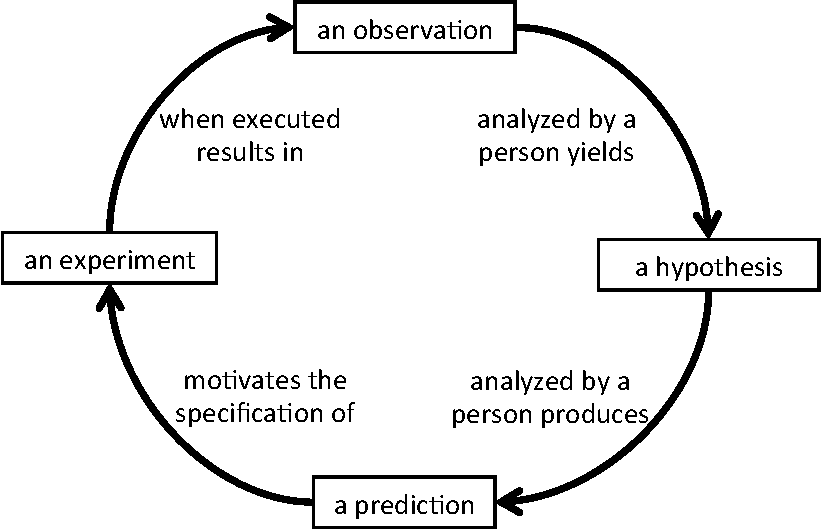
\includegraphics[width=.8\textwidth]{ScientificMethod}}\\\vspace{.3in}\Large 
    How can mathematics make this diagram meaningful?\\ 
    Как математика может придать смысл этой диаграмме?\normalsize
  }  

\begin{document}
\begin{russian}
\maketitle

%%%%%%%%%%%%%%%%%%%%%%%%%%%%%%%%%%%%%%%%%%%%%%%%%

\chapter*{Preface / Предисловие}

An early version of this book was put on line in February 2013 to serve as the textbook for my course \href{http://math.mit.edu/~dspivak/teaching/sp13/}{\text Category Theory for Scientists} taught in the spring semester of 2013 at MIT. During that semester, students provided me with hundreds of comments and questions, which led to a substantial improvement (and the addition of 50 pages) to the original document.

Ранняя версия данной книги была представлена в феврале 2013 в качестве учебника для моего курса \href{http://math.mit.edu/~dspivak/teaching/sp13/}{\text Теория категорий для ученых},%
\endnote{
В англоязычной литературе слово sciences обозначает как науки в целом, так и только естественные науки, в этом случае науки гуманитарные называют humanities [см. \href{https://en.wikipedia.org/wiki/The_Two_Cultures}{\text The Two Cultures}]. Выражая робкую надежду, что эта книга пригодится также и представителям последних, мы переводим science/scientist как наука/ученый вообще, не ограничивая их естественнонаучной направленностью.
} который читался в весеннем семестре 2013 в MIT. В течение семестра студенты передали мне сотни комментариев и вопросов, которые привели к существенному улучшению исходного текста (и к добавлению 50 страниц).

In the summer of 2013 I signed a contract with the MIT Press to publish a new version of this work under the title {\em Category Theory for the Sciences}. Because I am committed to the open source development model I insisted that a version of this book, namely the one you are reading, remain freely available online. The MIT Press version will of course not be free.

Летом 2013 я подписал контракт с MIT Press о публикации новой версии данной работы под заглавием {\em Теория категорий для наук}. Поскольку я являюсь приверженцем подхода открытого исходного кода, я настоял на том, чтобы отдельная версия этой книги, а именно — та, которую вы сейчас читаете, осталась доступной бесплатно онлайн.%
\endnote{
Данная книга не является единственной работой автора в области категорных оснований баз данных и представления знаний в информатике. Желающие увидеть полный список литературы могут обратиться к сайту Категорные Данные \cite{CDSite}, а также к персональной странице Д. И. Спивака \cite{SpHome}.
}

Other than the title, there are two main differences between the present version and the MIT Press version. The first difference is that I will do a full edit with the help of professional editors from the Press. The second difference is that I will write up solutions to the book's (approximately 280) exercises; some of these will be included in the published version, whereas the rest will be available by way of a password-protected page, accessible only to professors who teach the subject.

Помимо заголовка, есть еще два основных различия данной версии и версии MIT Press. Первое различие состоит в том, что я проведу кардинальное редактирование при помощи профессиональных редакторов. Второе различие — в том, что я напишу решения для упражнений этой книги (приблизительно 280); некоторые из них будут включены в опубликованную версию, тогда как остальные будут размещены на защищенной паролем странице, доступные только преподавателям, ведущим данный предмет. 

%%%%%%%% Chapter %%%%%%%%

\tableofcontents

%%%%%%%% Chapter %%%%%%%%

\chapter{Introduction / Введение}

The title page of this book contains a graphic that we reproduce here.
\begin{align}\label{dia:scientific method}
\dashbox{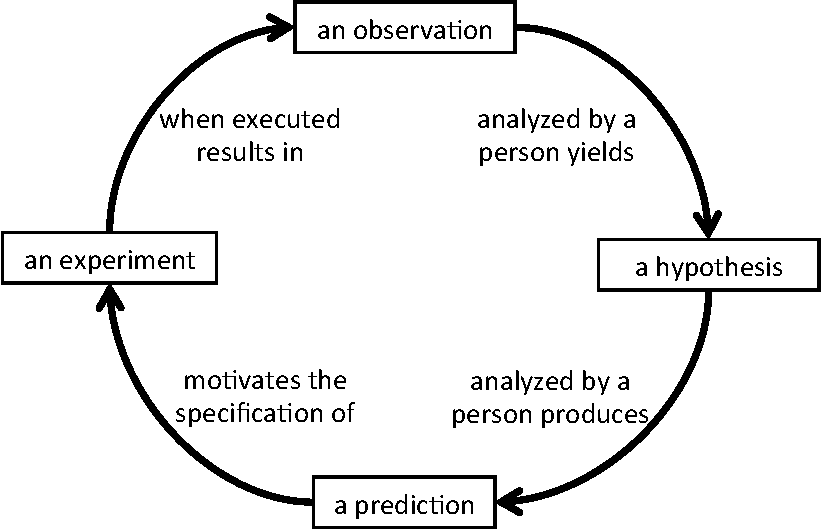
\includegraphics[width=.7\textwidth]{ScientificMethod}}
\end{align}
It is intended to evoke thoughts of the scientific method. \begin{quote}A hypothesis analyzed by a person produces a prediction, which motivates the specification of an experiment, which when executed results in an observation, which analyzed by a person yields a hypothesis.\end{quote}
This sounds valid, and a good graphic can be exceptionally useful for leading a reader through the story that the author wishes to tell. 

Титульная страница данной книги содержит рисунок, который мы воспроизводим ниже.
\begin{align}\label{dia:scientific method}
\dashbox{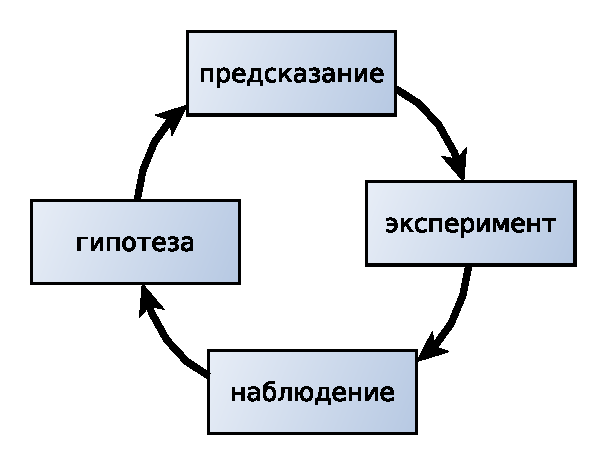
\includegraphics[width=.8\textwidth]{ScientificMethodRU}}
\end{align}
Он призван наводить на мысли о научном методе. \begin{quote}
Гипотеза, выведенная человеком при анализе, приводит к предсказанию, которое мотивирует описание эксперимента, который, после выполнения, приводит к наблюдениям, которые, будучи проанализированы человеком, приводят к гипотезе.\end{quote}
Это похоже на истину; кроме того, хорошая картинка может быть исключительно полезна, чтобы провести читателя сквозь историю, которую автор желает поведать.

Interestingly, a graphic has the power to evoke feelings of understanding, without really meaning much. The same is true for text: it is possible to use a language such as English to express ideas that are never made rigorous or clear. When someone says “I believe in free will,” what does she believe in? We may all have some concept of what she's saying — something we can conceptually work with and discuss or argue about. But to what extent are we all discussing the same thing, the thing she intended to convey?

Любопытный факт: картинка имеет способность вызывать ощущение понимания, не неся при этом особого смысла. То же верно и для слов: язык вроде английского способен выражать идеи, которые в принципе невозможно сделать строгими или ясными. Если некто заявляет «Я верю в свободу воли,» то во что некто верит? Все мы можем иметь некоторые представления о том, что этот некто говорит — такие, с которыми можно концептуально работать, рассуждать, аргументировать. Но до какой степени мы все будем обсуждать одну и ту же вещь, — вещь, которую некто собирался сообщить? 

Science is about agreement. When we supply a convincing argument, the result of this convincing is agreement. When, in an experiment, the observation matches the hypothesis — success! — that is agreement. When my methods make sense to you, that is agreement. When practice does not agree with theory, that is disagreement. Agreement is the good stuff in science; it's the high fives.

Суть науки — в согласии. Когда мы предлагаем убедительный аргумент,  результатом этой убедительности является согласие. Когда в ходе эксперимента наблюдения совпадают с гипотезой, — вот удача! — это согласие. Когда мои методы имеют смысл и для вас, это согласие. Когда же практика не соответствует теории, это несогласие. Согласие — вот лучшая материя в науке; оно подобно рукопожатию.%
\endnote{
Необходимо сказать пару слов о различении того, что приносит применение формальных методов вообще, и в чем особенность собственно теории категорий. Многое сказанное автором в предисловии относится к любым применениям математики в прикладных науках. Действительно, любая формализация заставляет выражать явным образом многое ранее интуитивно понятное, что представляет из себя зачастую значительный объем работы, а иногда и принципиально трудноразрешимые проблемы методологического характера. В результате в некоторые области математика проникла в меньше степени, чем в другие. Что же, однако, отличает подход, принятый в теории категорий? 
TODO ...(дать понятие об аксиоматическом методе, как реальном фундаменте математики, а также о различии логической парадигмы и алгебраической; теория - метатеория - модели)...
}

But it is easy to think we're in agreement, when really we're not. Modeling our thoughts on heuristics and pictures may be convenient for quick travel down the road, but we're liable to miss our turnoff at the first mile. The danger is in mistaking our convenient conceptualizations for what's actually there. It is imperative that we have the ability at any time to ground out in reality. What does that mean?

Однако легко попасть в ситуацию, когда мы думаем, будто согласны, но на самом деле это не так. Моделирование наших размышлений в эвристиках или картинках может быть удобно для быстрого движения напрямик, но нам самим придется нести ответственность, если мы пропустим нужный поворот на первой же миле. Опасность в том, что мы можем ошибочно принять удобство концепций за реальную картину. В любой момент необходимо иметь возможность привязаться к реальности. Что это означает? 

Data. Hard evidence. The physical world. It is here that science touches down and heuristics evaporate. So let's look again at the diagram on the cover. It is intended to evoke an idea of how science is performed. Is there hard evidence and data to back this theory up? Can we set up an experiment to find out whether science is actually performed according to such a protocol? To do so we have to shake off the stupor evoked by the diagram and ask the question: “what does this diagram intend to communicate?”

Данные. Железные подтверждения. Физический мир. Именно здесь наука приземляется, и испаряются эвристики. Так что давайте взглянем на диаграмму на обложке еще раз. Она предназначена вызывать идею о том, как делают науку. Но имеются ли железные подтверждения и данные, стоящие за подобной теорией? Способны ли мы организовать эксперимент для проверки того, что науку делают именно в соответствии с подобным протоколом? Чтобы сделать это, мы должны сбросить ступор, вызванный диаграммой, и задаться вопросом: «Что эта диаграмма должна нам сообщать?» 

In this course I will use a mathematical tool called {\em ologs}, or ontology logs, to give some structure to the kinds of ideas that are often communicated in pictures like the one on the cover. Each olog inherently offers a framework in which to record data about the subject. More precisely it encompasses a {\em database schema}, which means a system of interconnected tables that are initially empty but into which data can be entered. For example consider the olog below
$$\xymatrix{
\obox{}{.5in}{a mass}&&\obox{}{1.1in}{an object of mass $m$ held at height $h$ above the ground}\LAL{ll}{\footnotesize has as mass}\LA{rrdd}{\hspace{.4in}\parbox{1in}{\singlespace\footnotesize when dropped has as number of seconds till hitting the ground}}\LAL{dd}{\parbox{.7in}{\singlespace\footnotesize has as height in meters}}&&\\\\
&&\obox{}{1in}{a real number $h$}\ar@{}[uurr]|(.35){?}\ar[rr]_-{\sqrt{2h\div 9.8}}&\hspace{.3in}&\obox{}{.9in}{a real number}
}
$$
This olog represents a framework in which to record data about objects held above the ground, their mass, their height, and a comparison (the ?-mark in the middle) between the number of seconds till they hit the ground and a certain real-valued function of their height. We will discuss ologs in detail throughout this course.

В этом курсе я буду использовать математический инструмент, называемый {\em ологами} или же онтологическими записями, чтобы придать некую структуру тем видам идей, о которых зачастую сообщается в картинках, подобных той, что изображена на обложке. Каждый олог по своей сути представляет собой конструкцию, в которой записаны данные о предмете обсуждения. Более точно, они отражают {\em схему базы данных}, что означает систему взаимосвязанных таблиц, которые вначале пусты, но в которые могут быть внесены данные. Для примера рассмотрим такой олог 
$$\xymatrix{
\obox{}{.5in}{масса}&&\obox{}{1.1in}{объект массы $m$ удерживаемый на высоте $h$ над землей}\LAL{ll}{\footnotesize имеет массу}\LA{rrdd}{\hspace{.4in}\parbox{1in}{\singlespace\footnotesize при падении требуется определенное число секунд до ударения о землю}}\LAL{dd}{\parbox{.7in}{\singlespace\footnotesize имеет высоту в метрах}}&&\\\\
&&\obox{}{1in}{действительное число  $h$}\ar@{}[uurr]|(.35){\checkmark}\ar[rr]_-{\sqrt{2h\div 9.8}}&\hspace{.3in}&\obox{}{.9in}{действительное число  }
}
$$
Данный олог представляет собой конструкцию, в которой для объектов, находящихся над поверхностью земли, записаны: их масса, их высота и соответствие (отметка $\checkmark$ в середине) между числом секунд, за которое они достигают земли, с определенной действительнозначной функцией их высоты. Ологи мы детально обсудим по ходу этого курса. 

The picture in (\ref{dia:scientific method}) looks like an olog, but it does not conform to the rules that we lay out for ologs in Section \ref{sec:ologs}. In an olog, every arrow is intended to represent a mathematical function. It is difficult to imagine a function that takes in predictions and outputs experiments, but such a function is necessary in order for the arrow
$$\fbox{a prediction}\To{\tn{motivates the specification of}}\fbox{an experiment}
$$
in (\ref{dia:scientific method}) to make sense. To produce an experiment design from a prediction probably requires an expert, and even then the expert may be motivated to specify a different experiment on Tuesday than he is on Monday. But perhaps our criticism has led to a way forward: if we say that every arrow represents a function {\em when in the context of a specific expert who is actually doing the science at a specific time}, then Figure (\ref{dia:scientific method}) begins to make sense. In fact, we will return to the figure in Section \ref{sec:monads} (specifically Example \ref{ex:scientific method}), where background methodological context is discussed in earnest.

Картинка «научного метода» (\ref{dia:scientific method}) выглядит как олог, но она не соответствует правилам, которые мы изложим в Разделе \ref{sec:ologs}. В ологе каждая стрелка должна представлять математическую функцию. Трудно вообразить функцию, которая принимала бы предсказания и выдавала в результате эксперименты, но такая функция была бы необходима, чтобы стрелка 
$$\fbox{предсказание}\To{\tn{мотивирует спецификацию}}\fbox{эксперимент}
$$
в (\ref{dia:scientific method}) имела смысл. Чтобы разработать схему эксперимента по предсказанию нам, быть может, потребовался бы эксперт, но даже эксперт может решить предложить во вторник не тот эксперимент, который он предлагал в понедельник. Но, возможно, наша критика способна также предложить и путь вперед: если мы скажем, что каждая стрелка представляет функцию {\em в контексте конкретного эксперта, занимающегося наукой в конктерный момент времени}, тогда Рисунок (\ref{dia:scientific method}) приобретает смысл. А именно, мы еще будем возвращаться к диаграмме в Разделе \ref{sec:monads} (точнее, Пример \ref{ex:scientific method}), когда базовый методологический контекст будет обсуждаться более подробно. 

This course is an attempt to extol the virtues of a new branch of mathematics, called {\em category theory}, which was invented for powerful communication of ideas between different fields and subfields within mathematics. By powerful communication of ideas I actually mean something precise. Different branches of mathematics can be formalized into categories. These categories can then be connected together by functors. And the sense in which these functors provide powerful communication of ideas is that facts and theorems proven in one category can be transferred through a connecting functor to yield proofs of analogous theorems in another category. A functor is like a conductor of mathematical truth.

Данный курс является попыткой воздать должное достоинствам новой ветви математики, именуемой {\em теорией категорий}, которая была разработана для интенсивного обмена идеями между различными областями и подобластями математики. Под интенсивным обменом идеями я имею в виду нечто на самом деле точное. Разные ветви математики могут быть формализованы в виде отдельных категорий. Далее, эти категории могут быть связаны вместе функторами. И смысл, в котором эти функторы обеспечивают интенсивный обмен идеями — то, что факты и теоремы, доказанные в одной категории, могут быть перенесены при помощи соединяющего их функтора, порождая доказательства аналогичных теорем в другой категории. Функтор подобен проводнику математических истин. 

I believe that the language and toolset of category theory can be useful throughout science. We build scientific understanding by developing models, and category theory is the study of basic conceptual building blocks and how they cleanly fit together to make such models. Certain structures and conceptual frameworks show up again and again in our understanding of reality. No one would dispute that vector spaces are ubiquitous. But so are hierarchies, symmetries, actions of agents on objects, data models, global behavior emerging as the aggregate of local behavior, self-similarity, and the effect of methodological context.

Я верю, что язык и инструментарий теории категорий могут быть полезны во всей науке. Научное понимание мира строится на основе разработки сложных моделей, и теория категорий как раз изучает базовые концептуальные строительные блоки, а также то, как они могут быть четко состыкованы между собой при создании таких моделей. Определенные структуры и концептуальные конструкции обнаруживаются вновь и вновь в нашем понимании реальности. Никто не станет сомневаться в том, что векторные пространства вездесущи. Но таковы же и иерархии, симметрии, воздействия агентов на объекты, модели данных, глобальное поведение, возникающее при объединении локального поведения, самоподобие и методология явного учета побочных эффектов и контекста [в программировании].

Some ideas are so common that our use of them goes virtually undetected, such as set-theoretic intersections. For example, when we speak of a material that is both lightweight and ductile, we are intersecting two sets. But what is the use of even mentioning this set-theoretic fact? The answer is that when we formalize our ideas, our understanding is almost always clarified. Our ability to communicate with others is enhanced, and the possibility for developing new insights expands. And if we are ever to get to the point that we can input our ideas into computers, we will need to be able to formalize these ideas first.

Некоторые идеи настолько привычны, что наше использование их проходит практически незамеченным, — такие, как теоретико-множественное пересечение. Например, когда мы говорим, что материал легкий и пластичный, мы строим пересечение двух множеств. Но в чем польза от самого по себе упоминания такого теоретико-множественного факта? Ответ таков: когда мы формализуем свои идеи, наше понимание практически всегда проясняется. Улучшается наша способность общаться с другими, расширяются возможности новых открытий. И если мы хотим в будущем дойти до возможности ввода наших идей в компьютер, то прежде всего нам нужно уметь формализовывать эти идеи. 

It is my hope that this course will offer scientists a new vocabulary in which to think and communicate, and a new pipeline to the vast array of theorems that exist and are considered immensely powerful within mathematics. These theorems have not made their way out into the world of science, but they are directly applicable there. Hierarchies are partial orders, symmetries are group elements, data models are categories, agent actions are monoid actions, local-to-global\index{local-to-global} principles are sheaves, self-similarity is modeled by operads, context can be modeled by monads.

Я надеюсь, что данный курс предложит ученым новый словарь для мышления и общения, и широкую дорогу к громадному массиву теорем, которые уже существуют и рассматриваются как чрезвычайно мощные внутри математики. Эти теоремы еще не нашли проход к миру науки, но они там непосредственно применимы. Иерархии являются частичными порядками, симметрии — элементами групп, модели данных - категориями, воздействия агентов — действиями моноидов, локально-глобальные принципы — пучками, самоподобие моделируется операдами, контекст может быть смоделирован монадами. 

%%%%%% Section %%%%%%

\section{A brief history of category theory /  Краткая история теории категорий }

The paradigm shift brought on by Einstein's theory of relativity brought on the realization that there is no single perspective from which to view the world. There is no background framework that we need to find; there are infinitely many different frameworks and perspectives, and the real power lies in being able to translate between them. It is in this historical context that category theory got its start.%
\footnote{The following history of category theory is far too brief, and perhaps reflects more of the author's aesthetic than any kind of objective truth, whatever that may mean. Here are some much better references: \cite{Kro}, \cite{Mar1}, \cite{LM}.}


Сдвиг парадигмы, произведенный теорией относительности Эйнштейна, принес понимание того, что нет единой точки зрения на мир. Не существует основополагающей системы отсчёта, которую нам нужно найти; имеется бесконечно много различных систем отсчета и точек зрения, и настоящая мощь состоит в умении переходить между ними. В таком историческом контексте возникала теория категорий.%
\footnote{Нижеследующее описание истории теории категорий слишком кратко, и, возможно, отражает в большей степени авторское чувство прекрасного, чем любой вид объективной истины, что бы это ни значило. Вот некоторые значительно лучшие ссылки: \cite{Kro}, \cite{Mar1}, \cite{LM}.}%
\endnote{
TODO ...(дать краткий обзор областей теории категорий в исторической перспективе по темам: функторы, сопряжения, монады, алгебраические теории с категорной точки зрения, топосы как пример последних, теория высших категорий (гомотопии, кобордизмы, категория категорий), HoTT Воеводского)...
}

Category theory was invented in the early 1940s by Samuel Eilenberg\index{Eilenberg, Samuel} and Saunders Mac Lane.\index{Mac Lane, Saunders} It was specifically designed to bridge what may appear to be two quite different fields: topology and algebra. Topology is the study of abstract shapes such as 7-dimensional spheres; algebra is the study of abstract equations such as $y^2z=x^3-xz^2$. People had already created important and useful links (e.g. cohomology theory) between these fields, but Eilenberg and Mac Lane needed to precisely compare different links with one another. To do so they first needed to boil down and extract the fundamental nature of these two fields. But the ideas they worked out amounted to a framework that fit not only topology and algebra, but many other mathematical disciplines as well.

Теория категорий была создана в начале 1940-х Сэмюэлем Эйленбергом\index{Эйленберг, Сэмюэль} и Сондерсом Мак Лейном\index{Мак Лейн, Сондерс}. Она специально разрабатывалась для того, чтобы соединить две, на первый взгляд, совершенно различные области: топологию и алгебру. Топология изучает абстрактные формы, такие как 7-мерные сферы; алгебра изучает абстрактные уравнения, такие как $y^2z=x^3-xz^2$. Математики уже создали к тому времени важные и полезные связи (например, теорию когомологий) между этими областями, но Эйленбергу и Мак Лейну потребовалось провести точное сравнение различных связей друг с другом. Для этого им сперва потребовалось «выпарить и экстрагировать» фундаментальную природу этих двух областей. Однако идеи, на которых они проводили первые испытания, привели их к конструкции, которая подходила не только для топологии и алгебры, но с равным успехом была применима и для многих других математических дисциплин. 

At first category theory was little more than a deeply clarifying language for existing difficult mathematical ideas. However, in 1957 Alexander Grothendieck\index{Grothendieck!in history} used category theory to build new mathematical machinery (new cohomology theories) that granted unprecedented insight into the behavior of algebraic equations. Since that time, categories have been built specifically to zoom in on particular features of mathematical subjects and study them with a level of acuity that is simply unavailable elsewhere.

В самом начале теория категорий была не более, чем глубоко проясняющим языком для отдельных уже существующих трудных математических идей. Однако, в 1957 году Александр Гротендик\index{Гротендик!в истории} использовал теорию категорий для построения новой математической техники (новых когомологических теорий), которая предоставила беспрецендентное понимание поведения алгебраических уравнений. С тех пор категории стали строить специально для того, чтобы сосредоточиться на отдельных свойствах математических объектов и изучать их с такой четкостью, которая была ранее просто недоступна. 

Bill Lawvere\index{Lawvere, William} saw category theory as a new foundation for all mathematical thought. Mathematicians had been searching for foundations in the 19th century and were reasonably satisfied with set theory as {\em the foundation}. But Lawvere showed that the category of sets is simply a category with certain nice properties, not necessarily the center of the mathematical universe. He explained how whole algebraic theories can be viewed as examples of a single system. He and others went on to show that higher order logic was beautifully captured in the setting of category theory (more specifically toposes). It is here also that Grothendieck and his school worked out major results in algebraic geometry.

Билл Ловер\index{Ловер, Уилльям} увидел в теории категорий новые основания для всех математических построений. В поисках оснований математики находились еще в 19-м веке и ко временам Ловера были в достаточной степени удовлетворены использованием теории множеств в качестве {\em оснований}.%
\endnote{
TODO ...(неплохо бы объяснить читателю, что на математическом жаргоне называют «основаниями»)...
} Однако Ловер показал, что категория множеств это просто категория с определенными хорошими свойствами, а не обязательный центр математической вселенной. Он показал, как целые алгебраические теории могут рассматриваться в качестве примеров единой системы. Ему и другим удалось показать, что логика высших порядков прекрасно охватывается средствами теории категорий (конкретно, топосов). Пользуясь инструментами из этой же области, Гротендику и его школе удалось получить значительные результаты в алгебраической геометрии. 

In 1980 Joachim Lambek\index{Lambek, Joachim} showed that the types and programs used in computer science form a specific kind of category. This provided a new semantics for talking about programs, allowing people to investigate how programs combine and compose to create other programs, without caring about the specifics of implementation. Eugenio Moggi\index{Moggi, Eugenio} brought the category theoretic notion of monads into computer science to encapsulate ideas that up to that point were considered outside the realm of such theory.

В 1980 Иоахим Ламбек\index{Ламбек, Иоахим} показал, что типы и программы, используемые в информатике, образуют особого рода категорию. Это дало возможность обсуждать программы в рамках новой семантики, позволяя ученым исследовать, как программы комбинируются и соединяются в другие программы, не заботясь о специфике реализации. Эугенио Моджи\index{Моджи, Эугенио} принес в информатику теоретико-категорное понятие монад, которое инкапсулирует идеи, считавшиеся ранее недоступными для подобных теорий. 

It is difficult to explain the clarity and beauty brought to category theory by people like Daniel Kan\index{Kan, Daniel} and Andr\'{e} Joyal\index{Joyal, Andr\'{e}}. They have each repeatedly extracted the essence of a whole mathematical subject to reveal and formalize a stunningly simple yet extremely powerful pattern of thinking, revolutionizing how mathematics is done.

Трудно объяснить ясность и красоту, принесенные в теорию категорий такими людьми, как Дэниэл Кан\index{Кан, Дэниэл} и Андрэ Жуаяль\index{Жуаяль, Андрэ}. Каждый из них последовательно извлекал сущность целых областей математики, чтобы сделать их более явными и формализовать удивительно простые и в то же время чрезвычайно мощные способы мышления, революционизируя само занятие математикой. 

All this time, however, category theory was consistently seen by much of the mathematical community as ridiculously abstract. But in the 21st century it has finally come to find healthy respect within the larger community of pure mathematics. It is the language of choice for graduate-level algebra and topology courses, and in my opinion will continue to establish itself as the basic framework in which mathematics is done.

Все это время теория категорий последовательно считалась большинством специалистов до нелепости абстрактной. И все же, в 21-м веке она наконец находит здоровое уважение внутри все большего и большего сообщества чистых математиков. Это основной язык курсов по алгебре и топологии магистерского уровня, и, по моему мнению, он будет продолжать становиться тем каркасом, на основе которого делается вся математика. 

As mentioned above category theory has branched out into certain areas of science as well. Baez\index{Baez, John} and Dolan\index{Dolan, James} have shown its value in making sense of quantum physics, it is well established in computer science, and it has found proponents in several other fields as well. But to my mind, we are the very beginning of its venture into scientific methodology. Category theory was invented as a bridge and it will continue to serve in that role.

Как упоминалось выше, ответвления теории категорий проникли в некоторые другие области науки. Баэз\index{Баэз, Джон} и Долан\index{Долан, Джеймс} показали её важность в придании смысла квантовой физике, она уже основательно закрепилась в теоретической информатике, а также нашла сторонников в нескольких других областях. Тем не менее, по моему мнению, мы находимся только в самом начале ее пути в научную методологию. Теория категорий была создана в качестве связующего звена, и она продолжит исполнять эту роль. 

%%%%%% Section %%%%%%

\section{Intention of this book / Предназначение этой книги}

The world of {\em applied mathematics} is much smaller than the world of {\em applicable mathematics}. As alluded to above, this course is intended to create a bridge between the vast array of mathematical concepts that are used daily by mathematicians to describe all manner of phenomena that arise in our studies, and the models and frameworks of scientific disciplines such as physics, computation, and neuroscience.

Мир уж\'e существующей {\em примененной математики} (обычно называемой {\em прикладной}) значительно \'yже мира всей {\em применимой математики} [каламбур].%
\endnote{
Здесь и далее все краткие пояснения в квадратных скобках добавлены при переводе. Обычно они появляются в случае, если дословный перевод не способен отразить смысл исходного текста, а слишком художественный исказил бы его. Как говорит поговорка, «перевод - как женщина: если верен, то некрасив, а если красив, то неверен.»
} Как указывалось выше, этот курс предназначен создать мост между, с одной стороны, огромным массивом математических понятий, применяемых ежедневно математиками для описания возникающих в их исследованиях разнообразных феноменов, и, с другой стороны, моделями и конструкциями таких научных дисциплин, как физика, вычислительная математика, нейронаука. 

To the pure mathematician I'll try to prove that concepts such as categories, functors, natural transformations, limits, colimits, functor categories, sheaves, monads, and operads — concepts that are often considered too abstract for even math majors — can be communicated to scientists with no math background beyond linear algebra. If this material is as teachable as I think, it means that category theory is not esoteric but somehow well-aligned with ideas that already make sense to the scientific mind. Note, however, that this book is example-based rather than proof-based, so it may not be suitable as a reference for students of pure mathematics.

Что касается чистых математиков, им я попытаюсь доказать, что такие понятия, как категории, функторы, естественные преобразования, пределы, копределы, категории функторов, пучки, монады и операды — понятия, зачастую рассматриваемые как слишком абстрактные даже студентами старших курсов — могут использоваться для общения с учеными, чье математическое образование не выходит за рамки курса линейной алгебры. Если этот материал настолько доступен к преподаванию, насколько я думаю, то это означает, что теория категорий не является своего рода эзотерикой, но, в определенном смысле, несет в себе идеи, которые совпадают с уже существующими в уме любого ученого. Заметим, однако, что эта книга основана на примерах, а не на доказательствах, в результате чего она, возможно, не подойдет в качестве пособия для студентов-чистых математиков. 

To the scientist I'll try to prove the claim that category theory includes a formal treatment of conceptual structures that the scientist sees often, perhaps without realizing that there is well-oiled mathematical machinery to be employed. We will work on the structure of information; how data is made meaningful by its connections, both internal and outreaching, to other data. Note, however, that this book should most certainly not be taken as a reference on scientific matters themselves. One should assume that any account of physics, materials science, chemistry, etc. has been oversimplified.\index{a warning!oversimplified science} The intention is to give a flavor of how category theory may help us model scientific ideas, not to explain these ideas in a serious way.

Что касается ученых, им я попытаюсь доказать утверждение, что теория категорий включает в себя формальное изложение концептуальных структур, с которыми часто сталкивается ученый, возможно, не осознавая, что уже имеется готовый к употреблению «хорошо смазанный» математический механизм. Мы будем иметь дело со структурой информации; тем, как сделать данные осмысленными при помощи их связей, как внутренних, так и уходящих вовне. Заметим, однако, что данная книга совершенно определенно не должна рассматриваться как справочник по научным предметам самим по себе. Следует учитывать, что любое ознакомление с физикой, материаловедением и прочими, здесь дается в упрощенном виде\index{предупреждение!упрощенная наука}. Наша цель — дать почувствовать, как именно теория категорий может помочь моделировать научные идеи, а не серьезно объяснять сами эти идеи. 

Data gathering is ubiquitous in science. Giant databases are currently being mined for unknown patterns, but in fact there are many (many) known patterns that simply have not been catalogued. Consider the well-known case of medical records. A patient's medical history is often known by various individual doctor-offices but quite inadequately shared between them. Sharing medical records often means faxing a hand-written note or a filled-in house-created form between offices.

Сбор данных вездесущ в науке. Сейчас в гигантских базах данных ведется целенаправленный поиск ранее неизвестных взаимосвязей, и в то же время имеется огромное количество информации, которая просто еще не попала в эти каталоги. Рассмотрим хорошо известный случай медицинских записей. История болезни пациента хорошо известна различным отдельным медицинским заведениям, но совершенно неадекватно передается между ними. Обмен медицинскими записями зачастую означает передачу по факсу между заведениями рукописной справки или заполнения доморощенной формы. 

Similarly, in science there exists substantial expertise making brilliant connections between concepts, but it is being conveyed in silos of English prose known as journal articles. Every scientific journal article has a methods section, but it is almost impossible to read a methods section and subsequently repeat the experiment — the English language is inadequate to precisely and concisely convey what is being done.

Аналогично, в науке развит достаточный профессионализм в создании блистательных связей между понятиями, но он втискивается в прокрустово ложе естественного языка, известное как журнальные статьи. Каждая статья в научном журнале имеет методический раздел, но практически невозможно прочесть методический раздел и последовательно воспроизвести эксперимент, — английский язык неадекватен для точной и краткой передачи того, что же необходимо проделать. 

The first thing to understand in this course is that reusable methodologies can be formalized, and that doing so is inherently valuable. Consider the following analogy. Suppose you want to add up the area of a region in space (or the area under a curve). You break the region down into small squares, each of which you know has area $A$; then you count the number of squares, say $n$, and the result is that the region has an area of about $nA$. If you want a more precise and accurate result you repeat the process with half-size squares. This methodology can be used for any area-finding problem (of which there are more than a first-year calculus student generally realizes) and thus it deserves to be formalized. But once we have formalized this methodology, it can be taken to its limit and out comes integration by Riemann sums.

Первая вещь, которую следует понять из этого курса, — то, что повторно используемые методологии могут быть формализованы, и то, что делать это — существенно важно. Рассмотрим следующую аналогию. Предположим, мы хотим просуммировать площадь области в пространстве (или площадь под кривой). Мы разбиваем область на малые квадратики, каждый из которых имеет площадь $A$; затем мы подсчитываем число квадратиков, скажем $n$, и в результате получаем, что площадь равняется $nA$. Если мы хотим более точного результата, мы повторяем процедуру с квадратиками половинного размера. Эта методология может быть использована для любой задачи нахождения площади (которых гораздо больше, чем представляет себе студент-первокурсник, изучающий мат. анализ) и поэтому она заслуживает формализации. Но как только мы формализовали методологию, она может быть существенно улучшена, и отсюда получается интегрирование при помощи римановых сумм. 

I intend to show that category theory is incredibly efficient as a language for experimental design patterns, introducing formality while remaining flexible. It forms a rich and tightly woven conceptual fabric that will allow the scientist to maneuver between different perspectives whenever the need arises. Once one builds that fabric for oneself, he or she has an ability to think about models in a way that simply would not occur without it.  Moreover, putting ideas into the language of category theory forces a person to clarify their assumptions. This is highly valuable both for the researcher and for his or her audience.

Я собираюсь показать, что теория категорий невероятно эффективна как язык для экспериментальных дизайн-паттернов,%
\endnote{
TODO (и сюда дизайн-паттерны пробрались... или имеются в виду не они? уточнить!)
} одновременно вводя формальность и оставаясь гибкой. Она образует крепко сотканную ткань понятий, которая позволит ученым маневрировать между различными точками зрения, как только возникает необходимость. Как только некто строит подобную ткань для самого себя, он или она получает возможность думать о моделях способом, который бы без этого не возник. Более того, выражение идей в языке теории категорий заставляет человека сделать более ясными свои предположения. Это чрезвычайно ценно как для исследователя, так и для его аудитории. 

What must be recognized in order to find value in this course is that conceptual chaos is a major problem. Creativity demands clarity of thinking, and to think clearly about a subject requires an organized understanding of how its pieces fit together. Organization and clarity also lead to better communication with others. Academics often say they are paid to think and understand, but that is not true. They are paid to think, understand, and {\em communicate their findings}. Universal languages for science — languages such as calculus and differential equations, matrices, or simply graphs and pie-charts — already exist, and they grant us a cohesiveness that makes scientific research worthwhile. In this book I will attempt to show that category theory can be similarly useful in describing complex scientific understandings.

Для того, чтобы извлечь пользу из этого курса, необходимо увидеть, что хаос понятий представляет из себя существенную проблему. Творчество требует ясности мышления, а ясное мышление о предмете требует организованного понимания того, как части предмета соединяются вместе. Организованность и ясность также приводят к лучшему общению с другими. Академические работники часто заявляют, что им платят за то, чтобы они думали и понимали, но это неправда. Им платят за то, чтобы они думали, понимали и {\em сообщали о своих находках}. Универсальные языки для науки — такие, как анализ и дифференциальные уравнения, матрицы, или же просто графики и круговые диаграммы, — уже существуют, и именно они дают нам ту связность, что делает научные исследования стоящими потраченных на них усилий. В этой книге я попытаюсь показать, что и теория категорий может быть в равной степени полезна для описания сложных научных прозрений. 

%%%%%% Section %%%%%%

\section{What is requested from the student / Что потребуется от студента}

I will do my best to make clear the value of category theory in science, but I am not a scientist. To that end I am asking for your help in exploring how category theory may be useful in your specific field.

Я буду стараться изо всех сил сделать ясной ценность теории категорий в науке, но сам я не ученый. По этой причине я прошу вашей помощи в описании того, как теория категорий может быть полезна в вашей конкретной области. 

I also want you to recognize that the value of mathematics is not generally obvious at first. A good student learning a good subject with a good teacher will see something compelling almost immediately, but may not see how it will be useful in real life. This will come later. I hope you will work hard to understand even without yet knowing what its actual value in your life and research will be. Like a student of soccer is encouraged to spend hours juggling the ball when he or she could be practicing penalty shots, it is important to gain facility with the materials you will be using. Doing exercises is imperative for learning mathematics.

Я также хочу, чтобы вы поняли, что ценность математики не всегда сразу очевидна. Хороший студент, изучающий хороший предмет у хорошего преподавателя сможет понять нечто впечатляющее практически немедленно, но не сможет так же быстро понять, как это нечто может быть полезно в реальной жизни. Это придет позже. Я надеюсь, вы будете усердно трудиться над предметом, даже еще не понимая, в чем окажется его настоящая ценность в вашей жизни и исследованиях. Учащегося футболу заставляют проводить часы, упражняясь с мячом, вместо того, чтобы попрактиковаться в пенальти - ибо важно заранее обрести умения в избранном деле. Точно так же выполнение упражнений критически важно при обучении математике. 

%%%%%% Section %%%%%%

\section{Category theory references / Литература по теории категорий}

I wrote this book because the available books on category theory are almost all written for mathematicians (the rest are written for computer scientists). There is one book by Lawvere and Schanuel, called {\em Conceptual Mathematics} \cite{LS}, that offers category theory to a wider audience, but its style is not appropriate for this course. Still, it is very well written and clear.

Я написал эту книгу, потому что имеющиеся книги по теории категорий практически все написаны для математиков (остальные написаны для теоретиков информатики). Есть одна книга Ловера и Шануеля {\em Концептуальная математика} \cite{LS}, которая предлагает теорию категорий более широкой аудитории, но ее стиль не подходит для этого курса. Тем не менее, написана она очень хорошо и ясно. 

The “bible” of category theory is {\em Categories for the working mathematician} by Mac Lane \cite{Mac}. But as the title suggests, it was written for working mathematicians and will be quite opaque to my target audience. However, once a person has read my book, Mac Lane's book may become a valuable reference.

«Библия» теории категорий это {\em Категории для работающего математика} Мак Лейна \cite{Mac}. Но, как и предполагает ее заглавие, написана она для профессиональных математиков и будет совершенно непонятна моей целевой аудитории. Однако, после прочтения моей книги, книга Мак Лейна может стать ценным справочником.  

Other good books include Steve Awodey's book {\em Category theory} \cite{Awo} and Barr and Wells book {\em Category theory for computing science}, \cite{BW}.  A paper by Brown and Porter called  \href{http://pages.bangor.ac.uk/\%7Emas010/pdffiles/Analogy-and-Comparison.pdf}{\text Category Theory: an abstract setting for analogy and comparison} \cite{BP1} is more in line with the style of this book, only much shorter. Online, I find \href{http://www.wikipedia.org}{\text wikipedia} and a site called \href{http://ncatlab.org/nlab/show/HomePage}{\em the $n$lab} to be quite useful.

Другие хорошие книги включают книгу Стива Эводи {\em Теория категорий} \cite{Awo}, а также книгу Барра и Уэллса {\em Теория категорий для компьютерных наук}, \cite{BW}. Статья Брауна и Портера под названием  \href{http://pages.bangor.ac.uk/\%7Emas010/pdffiles/Analogy-and-Comparison.pdf}{\text Теория категорий: абстрактный инструмент для аналогий и сравнений} \cite{BP1} более соответствует стилю данной книги, но она значительно короче. Из онлайн-ресурсов, я считаю \href{http://www.wikipedia.org}{\text Википедию} и сайт под названием \href{http://ncatlab.org/nlab/show/HomePage}{$n$Lab} достаточно полезными. 

This book attempts to explain category theory by examples and exercises rather than by theorems and proofs. I hope this approach will be valuable to the working scientist.

Данная книга пытается изложить теорию категорий при помощи примеров и упражнений, а не теорем и доказательств. Я надеюсь, подобный подход окажется ценным для работающего ученого. 

%%%%%% Section %%%%%%

\section{(ниже идет скрытый текст)}

In a front page MIT news article on December 17, 2012 explained that {\em graphs}, systems of vertices and edges are “A simple tool for representing relationships between data, devices or almost anything else has ubiquitous applications in computer science.”\href{http://web.mit.edu/newsoffice/2012/explained-graphs-computer-science-1217.html}. Categories are graphs with one extra piece of structure: the ability to consider two paths, such as two different routes to the grocery store, to be equivalent. Reading it through, the MIT news article would have been more appropriately written about categories, had scientists been adequately aware of them. This is my hope for the course.

На первой странице выпуска MIT news за 17 декабря 2012 объясняется, что {\em графы}, системы вершин и ребер, будучи «простым инструментом для представления отношений между данными, устройствами или практически чем-угодно еще, имеют вездесущие приложения в информатике.»\href{http://web.mit.edu/newsoffice/2012/explained-graphs-computer-science-1217.html}. Категории являются графами с еще одним компонентом структуры: возможности считать два различных пути, таких как два различных маршрута к магазину, эквивалентными. Дочитав до конца, я убедился, что, если бы учёные были более адекватно информированы о категориях, данную статью для MIT было бы более уместно написать именно о них. Таковы мои надежды, которые я возлагаю на этот курс. 

These communication barriers are seen in businesses when one database “can't talk to” another — the two systems, though ostensibly containing information about the same topic, represent the information differently and therefore cannot be integrated without tremendous cost and overhaul. The barriers can be seen in teaching or training, when an expert has a hard time speaking in a language that the student is ready to understand. Finally, and most relevantly, they can be seen in science. Aside from teaching and training, there is the issue that researchers in even neighboring fields often find the barriers between disciplines to be insurmountable, and much of this has to do with differences in jargon.

? 

In math this is indeed the case: researchers in even neighboring fields do not understand what each other is doing. But the problem used to be much more pronounced. Category theory, invented in the 1940s has slowly been remedying this problem. Once a problem is formulated categorically it can be analyzed with respect to a growing body of ....

? 

What mathematics do scientists need to do their work? Calculus and its derivatives, such as differential equations; linear algebra and its span, which includes the likes of tensor analysis — these are invaluable to the process of doing science. In other words, to predicting the outputs of a system based on ones knowledge about it. But the working scientist has more to do than simply predict and understand. He or she needs to organize that the large amounts of information and knowledge, in such a way that it can be apprehended by others. No one is paid to think and understand; people are only paid to think, understand, and {\em communicate their findings}. Category theory is invaluable for the latter.

? 

But it goes further. If we were perfect thinkers then anything we thought once would be instantly recallable later, but this is not the case. We take notes so we can remember our earlier thoughts at a later time; I often find myself looking through old papers to remember ideas that used to be quite sharp for me, but which now are only vague memories. Thus we need to communicate not only to others but to our later selves. It turns out that if we come up with a good system for doing that, we end up not only using it to communicate to our selves 3 years later, but even 3 seconds later. A good organizational structure fundamentally changes how we do business.

? 

People often ask “is category theory just a language? Can anything be done with category theory that can't be done without it?” Consider a university like MIT; can the researchers here do anything that they couldn't do by themselves? Isn't it the minds themselves that are so valuable and unique? Perhaps not. Perhaps much of what goes on is enabled and made possible by the organizational structure of the university, which brings people together in the same space with the same rules, providing the  infrastructure necessary to do excellent work. The same is true in category theory: while many of the real advances come from domain-specific creativity, the language and toolset of category theory provides an infrastructure that enriches all involved. Category theory is mankind's most well-oiled conceptual machine to date.

Зачастую звучит вопрос: «Является ли теория категорий всего лишь языком? Можно ли сделать что-нибудь при помощи теории категорий, что невозможно сделать без нее?» Рассмотрим университет вроде MIT; может ли исследователь сделать здесь что-либо, что он не смог бы сделать самостоятельно? Не является ли [его] интеллект сам по себе тем, что ценно и уникально? Похоже, что нет. Похоже, большая часть из того, что происходит здесь, обусловлена организационной структурой университета, которая сводит людей в одно время в одном месте с одними и теми же правилами поведения, предлагая инфраструктуру, необходимую для качественной работы. То же верно и для теории категорий: хотя многое из действительно сделанного при помощи нее просходит из творчества в конкретных областях, язык и инструментарий теории категорий предлагает инфраструктуру, которая обогащает все, что ее использует. Теория категорий — это самая хорошо смазанная [т.е. эффективная] понятийная машина на сегодняшний день. 

%%%%%% Section %%%%%%

\section{Acknowledgments / Благодарности}

(ну, это скучный раздел, переведем потом) 

I would like to express my deep appreciation for the many scientists who I have worked with over the past five years. It all started with Paea LePendu who first taught me about databases when I was naively knocking on doors in the University of Oregon computer science department. This book would never have been written if Tristan Nguyen and Dave Balaban had not noticed my work and encouraged me to continue. Dave Balaban and Peter Gates have been my scientific partners since the beginning, working hard to understand what I'm offering and working just as hard to help me understand all that I'm missing. Peter Gates has deepened my understanding of data in profound ways.

 

I have also been tremendously lucky to know Haynes Miller, who made it possible for me set down at MIT, with the help of Clark Barwick and Jacob Lurie. I knew that MIT would be the best place in the world for me to pursue this type of research, and it has really come through. Researchers like Markus Buehler and his graduate students Tristan Giesa and Dieter Brommer have been a pleasure to work with, and the many materials science examples scattered throughout this book is a testament to how much our work together has influenced my thinking.

 

I'd also like to thank my collaborators and conversation partners with whom I have discussed subjects written about in this book. Other than people mentioned above, these include Steve Awodey, Allen Brown, Adam Chlipala, Carlo Curino, Dan Dugger, Henrik Forssell, David Gepner, Jason Gross, Bob Harper, Ralph Hutchison, Robert Kent, Jack Morava, Scott Morrison, David Platt, Joey Perricone, Dylan Rupel, Guarav Singh, Sam Shames, Nat Stapleton, Patrick Schultz, Ka Yu Tam, Ryan Wisnesky, Jesse Wolfson, and Elizabeth Wood.

 

I would like to thank Peter Kleinhenz and Peter Gates for reading this book and providing invaluable feedback before I began teaching the 18-S996 class at MIT in Spring 2013. In particular the cover image is a mild alteration of something Gates sent me to help motivate the book to scientists. I would also like to greatly thank the 18-S996 course grader Darij Grinberg, who was not only the best grader I've had in my 14 years of teaching, but gave me more comments than anyone else on the book itself. I'd also like to thank the students from the 18-S996 class at MIT who helped me find typos, pointed me to unclear explanations, and generally helped me improve the book in many ways. Other than the people listed above, these include Aaron Brookner, Leon Dimas, Dylan Erb, Deokhwan Kim, Taesoo Kim, Owen Lewis, Yair Shenfeld, and Adam Strandberg.

 

I would like to thank my teacher, Peter Ralston, who taught me to repeatedly question the obvious. My ability to commit to a project like this one and to see it to fruition has certainly been enhanced since studying with him.

 

Finally, I acknowledge my appreciation for support from the Office of Naval Research%
\footnote{Grant numbers: N000140910466, N000141010841, N000141310260}
without which this book would not have been remotely possible. I believe that their funding of basic research is an excellent way of ensuring that the US remains a global leader in the years to come.

 


%%%%%%%% Chapter %%%%%%%%

\chapter{The category of sets / Категория множеств}\label{chap:sets}

The theory of sets was invented as a foundation for all of mathematics. The notion of sets and functions serves as a basis on which to build our intuition about categories in general. In this chapter we will give examples of sets and functions and then move on to discuss commutative diagrams. At this point we can introduce ologs which will allow us to use the language of category theory to speak about real world concepts. Then we will introduce limits and colimits, and their universal properties. All of this material is basic set theory, but it can also be taken as an investigation of our first category, the {\em category of sets}, which we call $\Set$. We will end this chapter with some other interesting constructions in $\Set$ that do not fit into the previous sections.

Теория множеств разрабатывалась в качестве оснований всей математики. Понятие множества и функции служат основой, на которой строится наша интуиция о категориях вообще. В этой главе мы дадим примеры множеств и функций и затем перейдем к обсуждению коммутативных диаграмм. К тому моменту мы сможем ввести ологи, которые позволят нам использовать язык теории категорий, чтобы говорить о понятиях реального мира. Затем мы введем пределы и копределы и их универсальные свойства. Весь этот материал входит в область элементарной теории множеств, но он может также рассматриваться и как исследование нашей первой категории, {\em категории множеств}, которую мы назовем $\Set$. Мы закончим эту главу некоторыми другими интересными конструкциями в $Set$, которые не подходят к предыдущим разделам.%
\endnote{
TODO ...(возможно, пара слов о логической парадигме более конкретно: нужны ли нам понятия о предикатах и кванторах?)...
}

%%%%%% Section %%%%%%

\section{Sets and functions / Множества и функции}\index{set}\index{множество}

%%%% Subsection %%%%

\subsection{Sets / Множества}

In this course I'll assume you know what a set is.%
\endnote{
Мы можем предложить читателю несколько книг самого начального уровня о теории множеств. 

Златко Шпорер - Ох, эта математика! - М.: Педагогика, 1981. — 128с. 

Вавилов Н.А. - Не совсем наивная теория множеств, - Санкт-Петербург, 2008 год. 474 страницы
 
Николай Верещагин, Александр Шень - Начала теории множеств. - МЦНМО 2008 г.

} We can think of a set $X$ as a collection of things $x\in X$, each of which is recognizable as being in $X$ and such that for each pair of named elements $x,x'\in X$ we can tell if $x=x'$ or not.%
\footnote{Note that the symbol $x'$, read “x-prime”, has nothing to do with calculus or derivatives. It is simply notation that we use to name a symbol that is suggested as being somehow like $x$. This suggestion of kinship between $x$ and $x'$ is meant only as an aid for human cognition, and not as part of the mathematics.}
The set of pendulums is the collection of things we agree to call pendulums, each of which is recognizable as being a pendulum, and for any two people pointing at pendulums we can tell if they're pointing at the same pendulum or not. 

В этом курсе я буду предполагать, что вы знаете, что такое множество. Мы можем думать о множестве $X$ как о совокупности вещей $x\in X$, для каждой из которых мы можем проверить, находится ли она в $X$, и такой, что для каждой пары именованных элементов $x,x'\in X$ мы можем сказать, $x=x'$ или нет.%
\footnote{Заметим, что символ $x'$, читается «x-штрих», не имеет ничего общего с матанализом или производной. Это просто обозначение, которое мы используем, чтобы обозначить символ, в чем-то похожий на $x$. Такое предположение о родстве между $x$ и $x'$ имеет смысл только для целей удобства человеческого восприятия, а не как часть математики.}
Множество маятников это совокупность вещей, которые мы условились называть маятниками, про каждый из которых мы можем проверить, что это действительно маятник, и для любых двух людей, указывающих на маятники, мы можем сказать, показывают ли они на один и тот же маятник или нет. 

\begin{figure}
\begin{center}
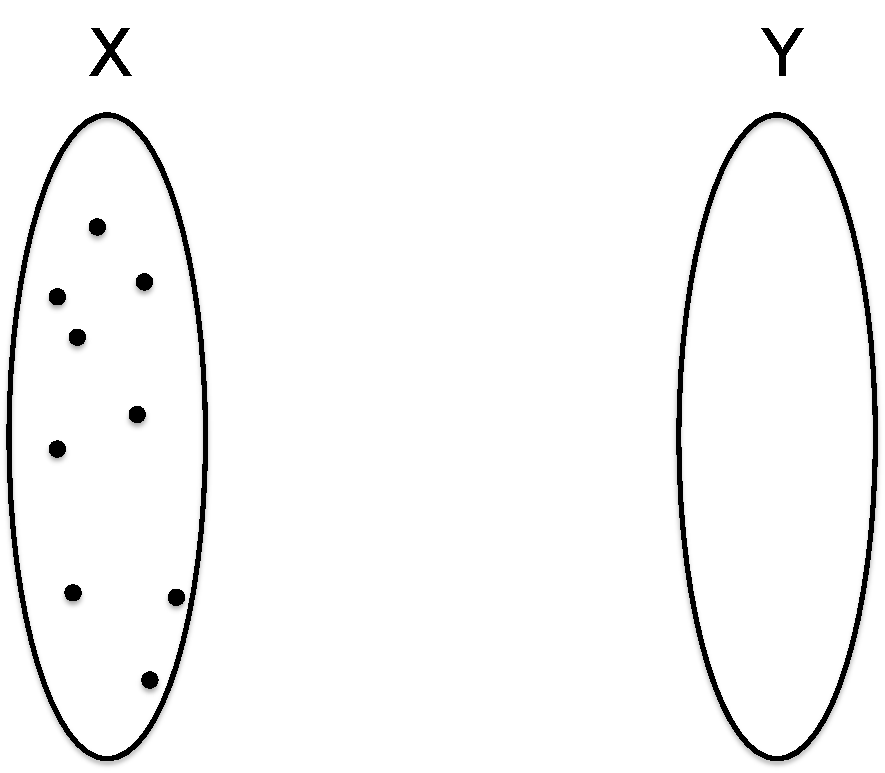
\includegraphics[height=2in]{aSet}
\end{center}
\caption{A set $X$ with $9$ elements and a set $Y$ with no elements, $Y=\emptyset$.}
\caption{Множество $X$ из $9$ элементов и множество $Y$ без элементов, $Y=\varnothing$.}
\end{figure}

\begin{notationENG}\label{not:basic math notation}
The symbol $\emptyset$\index{a symbol!$\emptyset$} denotes the set with no elements. The symbol $\NN$\index{a symbol!$\NN$} denotes the set of natural numbers, which we can write as 
$$\NN:=\{0,1,2,3,4,\ldots,877,\ldots\}.$$
The symbol $\ZZ$\index{a symbol!$\ZZ$} denotes the set of integers, which contains both the natural numbers and their negatives, 
$$\ZZ:=\{\ldots,-551,\ldots,-2,-1,0,1,2,\ldots\}.$$ 
\end{notationENG}
\begin{notationRUS}\label{not:basic math notation}

Символ $\varnothing$\index{символ!$\varnothing$} обозначает множество без элементов. Символ $\NN$\index{символ!$\NN$} обозначает множество натуральных чисел, которые мы можем записать как 
$$\NN:=\{0,1,2,3,4,\ldots,877,\ldots\}.$$
Символ $\ZZ$\index{символ!$\ZZ$} обозначает множество целых чисел, которое содержит как положительные, так и отрицательные числа, 
$$\ZZ:=\{\ldots,-551,\ldots,-2,-1,0,1,2,\ldots\}.$$ 

\end{notationRUS}
\begin{notationENG}\label{not:basic math notation}
If $A$ and $B$ are sets, we say that $A$ is a {\em subset}\index{subset} of $B$, and write $A\ss B$, if every element of $A$ is an element of $B$. So we have $\NN\ss\ZZ$. Checking the definition, one sees that for any set $A$, we have (perhaps uninteresting) subsets $\emptyset\ss A$ and $A\ss A$. We can use {\em set-builder notation}\index{set!set builder notation} to denote subsets. For example the set of even integers can be written $\{n\in\ZZ\|n\tn{ is even}\}$. The set of integers greater than $2$ can be written in many ways, such as $$\{n\in\ZZ\|n>2\} \hsp\tn{or}\hsp\{n\in\NN\|n>2\}\hsp\tn{or}\hsp\{n\in\NN\|n\geq 3\}.$$
\end{notationENG}

\begin{notationRUS}\label{not:basic math notation}
Если $A$ и $B$ — множества, мы называем $A$ {\em подмножеством}\index{подмножество} $B$, и пишем $A\ss B$ в случае, если каждый элемент $A$ является элементом $B$. Таким образом, имеем $\NN\ss\ZZ$. Проверив определение, можно убедиться, что у любого множества $A$ имеются (возможно, неинтересные) подмножества $\varnothing\ss A$ и $A\ss A$. Для обозначения подмножеств применяется специальная форма записи\index{множество!специальная форма записи}. Например, множество четных целых можно записать $\{n\in\ZZ\|n\tn{ четно}\}$. Множество целых, больших чем $2$ можно записать многими способами, такими как $$\{n\in\ZZ\|n>2\}, \hsp\tn{либо}\hsp\{n\in\NN\|n>2\}, \hsp\tn{либо}\hsp\{n\in\NN\|n\geq 3\}.$$
\end{notationRUS}

\begin{notationENG}\label{not:basic math notation}
The symbol $\exists$ means “there exists”.\index{a symbol!$\exists$} So we could write the set of even integers as $$\{n\in\ZZ\|n\tn{ is even}\}\hsp=\hsp\{n\in\ZZ\|\exists m\in\ZZ\tn{ such that } 2m=n\}.$$ The symbol $\exists!$\index{a symbol!$\exists$!} means “there exists a unique”. So the statement “$\exists! x\in\RR\tn{ such that } x^2=0$” means that there is one and only one number whose square is 0. Finally, the symbol $\forall$ means “for all”.\index{a symbol!$\forall$} So the statement “$\forall m\in\NN\;\exists n\in\NN\tn{ such that } m<n$” means that for every number there is a bigger one.
\end{notationENG}

\begin{notationRUS}\label{not:basic math notation}
Символ $\exists$ означает «существует».\index{символ!$\exists$} Таким образом мы можем записать множество четных чисел $$\{n\in\ZZ\|n\tn{ четно}\}\hsp=\hsp\{n\in\ZZ\|\exists m\in\ZZ\tn{ такое, что } 2m=n\}.$$ Символ $\exists!$\index{символ!$\exists$!} означает «существует единственный». Таким образом утверждение «$\exists! x\in\RR\tn{ такой, что } x^2=0$» означает, что имеется одно и только одно число, равное в квадрате $0$. Наконец, символ $\forall$ означает «для всех», «для каждого».\index{символ!$\forall$} Таким образом утверждение «$\forall m\in\NN\;\exists n\in\NN\tn{ такой, что } m<n$» означает, что для каждого числа имеется большее него. 
\end{notationRUS}

\begin{notationENG}\label{not:basic math notation}
As you may have noticed, we use the colon-equals notation “$A:=XYZ$” to mean something like “define $A$ to be $XYZ$”.\index{символ!:=} That is, a colon-equals declaration is not denoting a fact of nature (like $2+2=4$), but a choice of the speaker. It just so happens that the notation above, such as $\NN:=\{0,1,2,\ldots\}$, is a widely-held choice.
\end{notationENG}

\begin{notationRUS}\label{not:basic math notation}
Как вы могли заметить, мы пользуемся записью «двоеточие-равно» $A:=XYZ$, чтобы обозначить нечто вроде «определим $A$ как $XYZ$».\index{символ!:=} То есть, объявление чего-то в виде двоеточие-равно не означает новый факт о мире (вроде $2+2=4$), а всего лишь выбор обозначения говорящим. Просто так получилось, что обозначения выше, такие как $\NN:=\{0,1,2,\ldots\}$, широко используются. 
\end{notationRUS}

\begin{exerciseENG}Let $A=\{1,2,3\}$. What are all the subsets of $A$? Hint: there are 8.\end{exerciseENG}

\begin{exerciseRUS}Пусть $A=\{1,2,3\}$. Каковы все подмножества $A$? Подсказка: их ровно $8$. \end{exerciseRUS}

%%%% Subsection %%%%

\subsection{Functions / Функции}\label{sec:functions}

If $X$ and $Y$ are sets, then a {\em function $f$ from $X$ to $Y$},\index{function} denoted $f\taking X\to Y$, is a mapping that sends each element $x\in X$ to an element of $Y$, denoted $f(x)\in Y$. We call $X$ the {\em domain}\index{function!domain} of the function $f$ and we call $Y$ the {\em codomain}\index{function!codomain} of $f$. 

Если $X$ и $Y$ — множества, то {\em функция $f$ из $X$ в $Y$}\index{функция}, обозначаемая $f\taking X\to Y$, это отображение, которое переводит каждый элемент $x\in X$ в элемент $Y$, обозначаемый $f(x)\in Y$. Мы называем $X$ {\em областью определения}\index{функция!область определения} (или просто {\em областью}) для функции $f$, а $Y$ — {\em областью значений}\index{функция!область значений} (или просто {\em кообластью}) для $f$.  

\begin{align}\label{dia:setmap}
\parbox{2.3in}{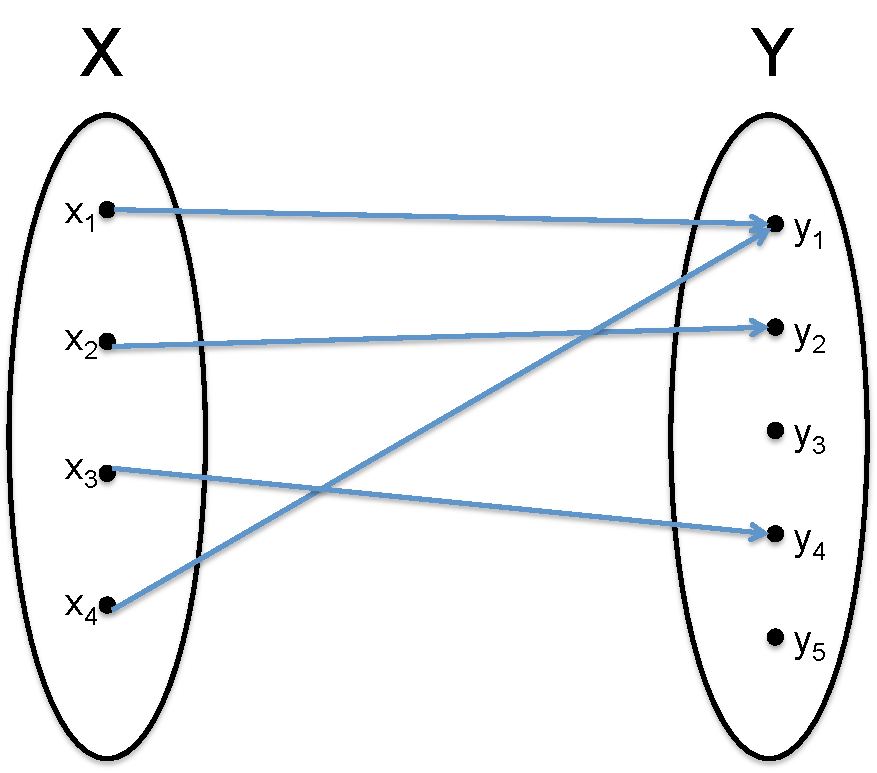
\includegraphics[height=2in]{SetMap}}
\end{align}

Note that for every element $x\in X$, there is exactly one arrow emanating from $x$, but for an element $y\in Y$, there can be several arrows pointing to $y$, or there can be no arrows pointing to $y$. 

Заметим, что для каждого элемента $x\in X$ имеется в точности одна стрелка, исходящая из $x$, в то же время для элемента $y\in Y$ может быть несколько стрелок, указывающих на $y$, или их вообще может не быть.

\begin{applicationENG}\label{app:force-extension}\index{materials!force-extension curves}
In studying the mechanics of materials, one wishes to know how a material responds to tension. For example a rubber band responds to tension differently than a spring does. To each material we can associate a \href{http://en.wikipedia.org/wiki/Stress–strain_curve}{\text force-extension curve}, recording how much force the material carries when extended to various lengths. Once we fix a methodology for performing experiments, finding a material's force-extension curve would ideally constitute a function from the set of materials to the set of curves.%
\footnote{In reality, different samples of the same material, say samples of different sizes or at different temperatures, may have different force-extension curves. If we want to see this as a true function whose codomain is curves it should have as domain something like the set of material samples.}
\end{applicationENG}

\begin{applicationRUS}\label{app:force-extension}\index{материалы!диаграмма деформирования}
При изучении сопротивления материалов [часть механики деформируемого твёрдого тела] стремятся исследовать, как материал реагирует на напряжение [сжатие и растяжение]. Например, резиновая лента реагирует на напряжение не так, как пружина. С каждым материалом мы можем ассоциировать \href{https://ru.wikipedia.org/wiki/%D0%94%D0%B8%D0%B0%D0%B3%D1%80%D0%B0%D0%BC%D0%BC%D0%B0_%D0%B4%D0%B5%D1%84%D0%BE%D1%80%D0%BC%D0%B8%D1%80%D0%BE%D0%B2%D0%B0%D0%BD%D0%B8%D1%8F}{\text диаграмму деформирования}, описывающую, силу какой величины материал выдерживает, будучи растянут до различной длины. Как только мы зафиксировали методологию проведения экспериментов, нахождение кривой сила-растяжение для данного материала идеальным образом образует функцию из множества материалов в множество кривых.%
\footnote{В действительности, различные образцы одного и того же материала, скажем, образцы различного размера или при различной температуре, могут иметь различные кривые сила-растяжение. Если мы хотим увидеть здесь настоящую функцию с областью значений «кривые», мы должны взять в качестве области определения нечто вроде «образцы материала».} 
\end{applicationRUS}

\begin{exerciseENG}
Here is a simplified account of how the \href{http://en.wikipedia.org/wiki/Retina}{\text brain receives light}. The eye contains about 100 million photoreceptor (PR) cells. Each connects to a retinal ganglion (RG) cell. No PR cell connects to two different RG cells, but usually many PR cells can attach to a single RG cell. 

Let $PR$ denote the set of photoreceptor cells and let $RG$ denote the set of retinal ganglion cells. 
\sexc According to the above account, does the connection pattern constitute a function $RG\to PR$, a function $PR\to RG$ or neither one? 
\next Would you guess that the connection pattern that exists between other areas of the brain are “function-like”?
\endsexc
\end{exerciseENG}

\begin{exerciseRUS}
Ознакомимся упрощенно с тем, как \href{https://ru.wikipedia.org/wiki/%D0%A1%D0%B5%D1%82%D1%87%D0%B0%D1%82%D0%BA%D0%B0}{\text мозг воспринимает свет}. Глаз содержит около 100 миллионов светочувствительных нейронов (фоторецепторов, PR). Каждый из них связан с ганглионарным нейроном (RG) [не напрямую]. Ни один PR не связан с двумя RG, в то же время с единственным RG может быть связано много PR.

Пусть $PR$ обозначает множество фоторецепторов и пусть $RG$ обозначает множество ганглионарных нейронов сетчатки. 
\sexc В соответствии с информацией выше, образует ли схема связей нейронов функцию $RG\to PR$, функцию $PR\to RG$ или ни одну из них? 
\next Как вы думаете, могут ли схемы связей между другими областями мозга быть «функциеподобными»? 
\endsexc 
\end{exerciseRUS}

\begin{exampleENG}\label{ex:subset as function}\index{subset!as function}
Suppose that $X$ is a set and $X'\ss X$ is a subset. Then we can consider the function $X'\to X$ given by sending every element of $X'$ to “itself” as an element of $X$. For example if $X=\{a,b,c,d,e,f\}$ and $X'=\{b,d,e\}$ then $X'\ss X$ and we turn that into the function $X'\to X$ given by $b\mapsto b, d\mapsto d, e\mapsto e$.%
\footnote{This kind of arrow,\;\;$\mapsto$\;\;, is read aloud as “maps to”. A function $f\taking X\to Y$ means a rule for assigning to each element $x\in X$ an element $f(x)\in Y$. We say that “$x$ maps to $f(x)$” and write $x\mapsto f(x)$.}\index{a symbol!$\mapsto$}

As a matter of notation, we may sometimes say something like the following: Let $X$ be a set and let $i\taking X'\ss X$ be a subset. Here we are making clear that $X'$ is a subset of $X$, but that $i$ is the name of the associated function.
\end{exampleENG}

\begin{exampleRUS}\label{ex:subset as function}\index{подмножество!как функция}
Предположим, $X$ — множество и $X'\ss X$ — подмножество. Тогда мы можем рассмотреть функцию $X'\to X$, заданную превращением каждого элемента $X'$ в себя, но уже как элемент $X$. Например, если $X=\{a,b,c,d,e,f\}$ и $X'=\{b,d,e\}$, то $X'\ss X$ и мы получаем отсюда функцию $X'\to X$, заданную как $b\mapsto b, d\mapsto d, e\mapsto e$.%
\footnote{Такой вид стрелочки,\;\;$\mapsto$\;\;, читается вслух как «переходит в». Функция $f\taking X\to Y$ означает правило сопоставления каждому элементу $x\in X$ элемента $f(x)\in Y$. При этом мы говорим, что «$x$ переходит в $f(x)$» и пишем $x\mapsto f(x)$.}\index{символ!$\mapsto$}

Что касается обозначений, мы можем сказать иногда нечто вроде следующего: «Пусть $X$ — множество и пусть $i\taking X'\ss X$ — подмножество». Здесь мы ясно говорим, что $X'$ это подмножество $X$, а также, что $i$ это имя соответствующей функции.
\end{exampleRUS}

\begin{exerciseENG}
Let $f\taking\NN\to\NN$ be the function that sends every natural number to its square, e.g. $f(6)=36$. First fill in the blanks below, then answer a question.
\sexc $2\mapsto\ul{\hspace{.5in}}$
\next $0\mapsto\ul{\hspace{.5in}}$
\next $-2\mapsto\ul{\hspace{.5in}}$
\next $5\mapsto\ul{\hspace{.5in}}$
\next Consider the symbol $\to$ and the symbol $\mapsto$. What is the difference between how these two symbols are used in this book?
\endsexc
\end{exerciseENG}

\begin{exerciseRUS}
Пусть $f\taking\NN\to\NN$ — функция, переводящая каждое натуральное число в его квадрат, например $f(6)=36$. Заполните вначале пустые места ниже, затем ответьте на вопрос.
\sexc $2\mapsto\ul{\hspace{.5in}}$
\next $0\mapsto\ul{\hspace{.5in}}$
\next $-2\mapsto\ul{\hspace{.5in}}$
\next $5\mapsto\ul{\hspace{.5in}}$
\next Рассмотрим символ $\to$ и символ $\mapsto$. В чем разница между тем, как эти два символа используются в данной книге?
\endsexc
\end{exerciseRUS}

Given a function $f\taking X\to Y$, the elements of $Y$ that have at least one arrow pointing to them are said to be {\em in the image} of $f$; that is we have \index{image}
\begin{align}\label{dia:image}
\im(f):=\{y\in Y\| \exists x\in X \tn{ such that } f(x)=y\}.
\end{align} 

Для заданной функции $f\taking X\to Y$, те элементы $Y$, для которых имеется по крайней мере одна стрелка, указывающая на них, называются лежащими {\em в образе} $f$; получаем \index{образ}
\begin{align}\label{dia:image}
\im(f):=\{y\in Y\| \exists x\in X \tn{ такой, что } f(x)=y\}.
\end{align}

\begin{exerciseENG}
If $f\taking X\to Y$ is depicted by (\ref{dia:setmap}) above, write its image, $\im(f)$ as a set.
\end{exerciseENG}

\begin{exerciseRUS}
Для $f\taking X\to Y$, изображенной на (\ref{dia:setmap}) выше, запишите ее образ $\im(f)$ в виде множества.
\end{exerciseRUS}

Given a function $f\taking X\to Y$ and a function $g\taking Y\to Z$, where the codomain of $f$ is the same set as the domain of $g$ (namely $Y$), we say that $f$ and $g$ are composable $$X\Too{f}Y\Too{g}Z.$$ The {\em composition of $f$ and $g$}\label{function composition}\index{function!composition}\index{composition!of functions}\index{a symbol!$\circ$} is denoted by $g\circ f\taking X\to Z$. 

Если заданы функция $f\taking X\to Y$ и функция $g\taking Y\to Z$, где кообласть $f$ совпадает с областью $g$ (то есть, $Y$), мы говорим, что $f$ и $g$ соединимы. $$X\Too{f}Y\Too{g}Z.$$ {\em Композиция $f$ и $g$}\label{function composition}\index{функция!композиция}\index{композиция!функций}\index{символ!$\circ$} обозначается $g\circ f\taking X\to Z$. 

\begin{figure}[h]
\begin{center}
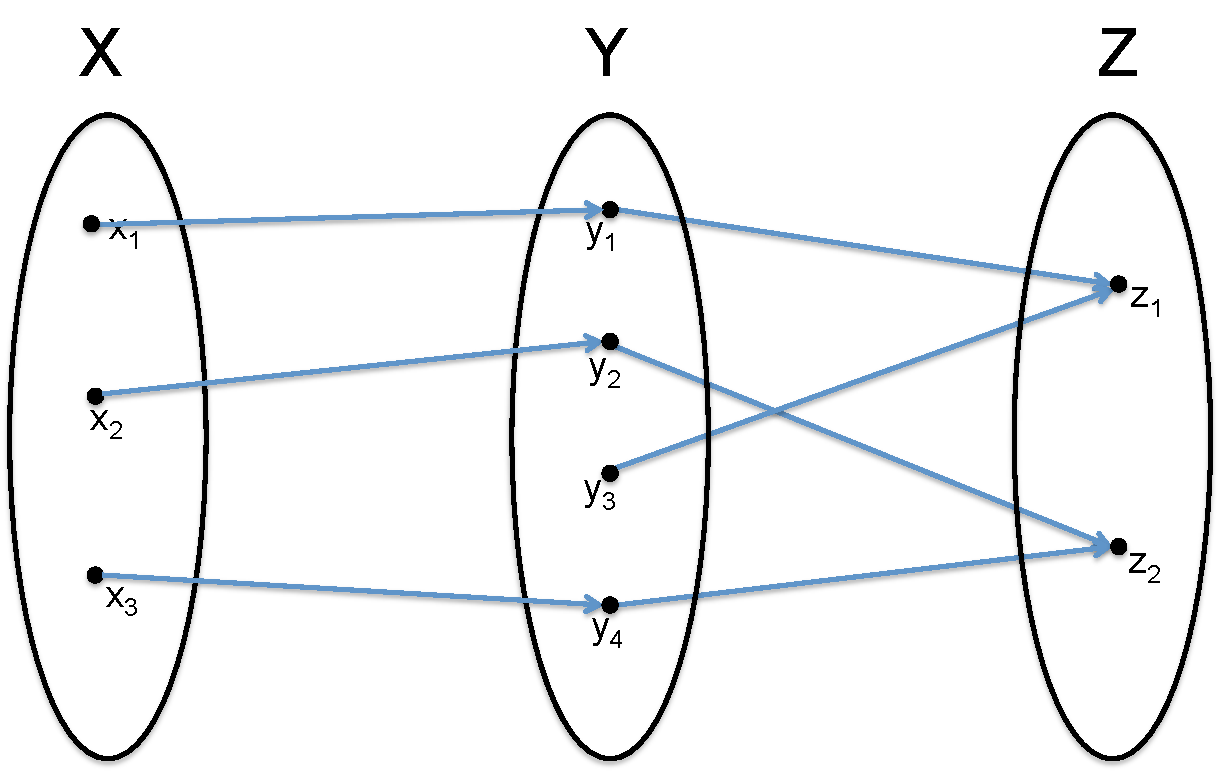
\includegraphics[height=2in]{composition}
\end{center}
\caption{Functions $f\taking X\to Y$ and $g\taking Y\to Z$ compose to a function $g\circ f\taking X\to Z$; just follow the arrows.}
\caption{Из функций $f\taking X\to Y$ и $g\taking Y\to Z$, просто следуя по стрелочкам, получается композиция — функция $g\circ f\taking X\to Z$}
\end{figure}

Let $X$ and $Y$ be sets. We write $\Hom_\Set(X,Y)$\index{a symbol!$\Hom_\Set$} to denote the set of functions $X\to Y$.%
\footnote{The strange notation $\Hom_\Set(-,-)$ will make more sense later, when it is seen as part of a bigger story.} 
Note that two functions $f,g\taking X\to Y$ are equal\index{function!equality of} if and only if for every element $x\in X$ we have $f(x)=g(x)$. 

Пусть $X$ и $Y$ — множества. Мы записываем $\Hom_\Set(X,Y)$\index{символ!$\Hom_\Set$} для обозначения множества функций $X\to Y$.%
\footnote{Странное обозначение $\Hom_\Set(-,-)$ обретет смысл позже, когда мы увидим его как часть большой картины.} 
Заметим, что две функции $f,g\taking X\to Y$ считаются равными\index{функция!равенство}, если и только если для каждого элемента $x\in X$ верно равенство $f(x)=g(x)$. 

\begin{exerciseENG}
Let $A=\{1,2,3,4,5\}$ and $B=\{x,y\}.$ 
\sexc How many elements does $\Hom_\Set(A,B)$ have? 
\next How many elements does $\Hom_\Set(B,A)$ have?
\endsexc
\end{exerciseENG}

\begin{exerciseRUS}
Пусть $A=\{1,2,3,4,5\}$ и $B=\{x,y\}.$ 
\sexc Сколько элементов имеется в $\Hom_\Set(A,B)$? 
\next Сколько элементов имеется в $\Hom_\Set(B,A)$?
\endsexc
\end{exerciseRUS}

\begin{exerciseENG}~
\sexc Find a set $A$ such that for all sets $X$ there is exactly one element in $\Hom_\Set(X,A)$. Hint: draw a picture of proposed $A$'s and $X$'s.
\next Find a set $B$ such that for all sets $X$ there is exactly one element in $\Hom_\Set(B,X)$.
\endsexc 
\end{exerciseENG}

\begin{exerciseRUS}~
\sexc Найти множество $A$ такое, что для всех множеств $X$ в $\Hom_\Set(X,A)$ имеется в точности один элемент. Подсказка: нарисовать картинку с пробными $A$ и $X$.
\next Найти множество $B$ такое, что для всех множеств $X$ в $\Hom_\Set(B,X)$ имеется в точности один элемент.
\endsexc 
\end{exerciseRUS}

For any set $X$, we define the {\em identity function on $X$}\index{function!identity}, denoted $\id_X\taking X\to X$, to be the function such that for all $x\in X$ we have $\id_X(x)=x$.\index{a symbol!$\id_X$}

Для любого множества $X$, мы определим {\em тождественную функцию на $X$}\index{функция!тождественная}, обозначаемую $\id_X\taking X\to X$, как функцию такую, что для всех $x\in X$ верно равенство $\id_X(x)=x$.\index{символ!$\id_X$}

\begin{definitionENG}[Isomorphism]\label{def:iso in set} 
Let $X$ and $Y$ be sets. A function $f\taking X\to Y$ is called an {\em isomorphism}\index{function!isomorphism}\index{isomorphism!of sets}, denoted $f\taking X\To{\iso}Y$, if there exists a function $g\taking Y\to X$ such that $g\circ f=\id_X$ and $f\circ g=\id_Y$. We also say that $f$ is {\em invertible} and we say that $g$ is {\em the inverse}\index{function!inverse} of $f$. If there exists an isomorphism $X\To\iso Y$ we say that $X$ and $Y$ are {\em isomorphic} sets and may write $X\iso Y$. \index{a symbol!$\iso$}
\end{definitionENG}

\begin{definitionRUS}[Изоморфизм]\label{def:iso in set}
Пусть $X$ и $Y$ — множества. Функция $f\taking X\to Y$ называется {\em изоморфизмом}\index{функция!изоморфизм}\index{изоморфизм!множеств}, что обозначается как $f\taking X\To{\iso}Y$, если существует функция $g\taking Y\to X$ такая, что $g\circ f=\id_X$ и $f\circ g=\id_Y$. Мы также говорим, что $f$ является {\em обратимой}, и что $g$ является {\em обратной}\index{функция!обратная} к $f$. Если существует изоморфизм $X\To\iso Y$, то мы говорим, что $X$ и $Y$ являются {\em изоморфными} множествами, и записываем это как $X\iso Y$. \index{символ!$\iso$}
\end{definitionRUS}

\begin{exampleENG}
If $X$ and $Y$ are sets and $f\taking X\to Y$ is an isomorphism then the analogue of Diagram \ref{dia:setmap} will look like a perfect matching, more often called a {\em one-to-one correspondence}\index{one-to-one correspondence}\index{correspondence!one-to-one}. That means that no two arrows will hit the same element of $Y$, and every element of $Y$ will be in the image. For example, the following depicts an isomorphism $X\To{\iso}Y$.
\end{exampleENG}

\begin{exampleRUS}
Если $X$ и $Y$ — множества и $f\taking X\to Y$ — изоморфизм, то аналог Диаграммы \ref{dia:setmap} будет выглядеть как идеальное совпадение, чаще называемое {\em соответствием один-к-одному}\index{соответствие один-к-одному}\index{соответствие!один-к-одному}. Это означает, что никакие две стрелки не попадают в один элемент $Y$, и что каждый элемент $Y$ находится в образе. Например, ниже изображен изоморфизм $X\To{\iso}Y$.
\end{exampleRUS}

\begin{align}\label{dia:setmapiso}
\parbox{2.3in}{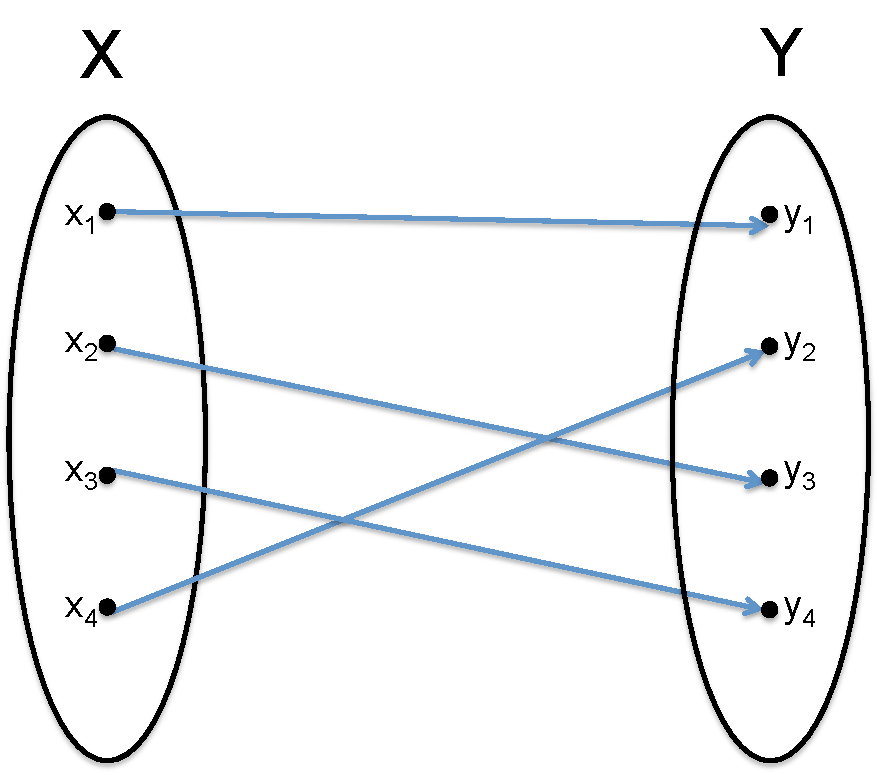
\includegraphics[height=2in]{SetMapIso}}
\end{align}

\begin{applicationENG}\label{app:DNA RNA}\index{RNA transcription}
There is an isomorphism between the set $\tn{Nuc}_\tn{DNA}$ of \href{http://en.wikipedia.org/wiki/Nucleotides}{\text nucleotides} found in DNA and the set $\tn{Nuc}_\tn{RNA}$ of nucleotides found in RNA. Indeed both sets have four elements, so there are 24 different isomorphisms. But only one is useful. Before we say which one it is, let us say there is also an isomorphism $\tn{Nuc}_\tn{DNA}\iso\{A,C,G,T\}$ and an isomorphism $\tn{Nuc}_\tn{RNA}\iso\{A,C,G,U\}$, and we will use the letters as abbreviations for the nucleotides. 

The convenient isomorphism $\tn{Nuc}_\tn{DNA}\To{\iso}\tn{Nuc}_\tn{RNA}$ is that given by RNA transcription; it sends 
$$A\mapsto U, C\mapsto G, G\mapsto C, T\mapsto A.$$ 
(See also Application \ref{app:polymerase}.) There is also an isomorphism $\tn{Nuc}_\tn{DNA}\To{\iso}\tn{Nuc}_\tn{DNA}$ (the matching in the double-helix) given by 
$$A\mapsto T, C\mapsto G, G\mapsto C, T\mapsto A.$$

Protein production can be modeled as a function from the set of 3-nucleotide sequences to the set of eukaryotic amino acids. However, it cannot be an isomorphism because there are $4^3=64$ triplets of RNA nucleotides, but only 21 eukaryotic amino acids. 
\end{applicationENG}

\begin{applicationRUS}\label{app:DNA RNA}\index{РНК транскрипция}
Имеется изоморфизм между множеством $\tn{Nuc}_\tn{DNA}$, состоящим из  \href{https://ru.wikipedia.org/wiki/%D0%9D%D1%83%D0%BA%D0%BB%D0%B5%D0%BE%D1%82%D0%B8%D0%B4%D1%8B}{\text нуклеотидов}, встречающихся в ДНК, и множеством $\tn{Nuc}_\tn{RNA}$ нуклеотидов, встречающихся в РНК. На самом деле в обоих множествах по четыре элемента, так что [всего между ними] имеется 24 различных изоморфизма. И только один из них нам нужен! Прежде, чем мы укажем, какой именно, давайте заметим, что имеются также изоморфизм $\tn{Nuc}_\tn{DNA}\iso\{A,C,G,T\}$ и изоморфизм $\tn{Nuc}_\tn{RNA}\iso\{A,C,G,U\}$, и что мы используем буквы для сокращения названий нуклеотидов. 

Подходящий изоморфизм $\tn{Nuc}_\tn{DNA}\To{\iso}\tn{Nuc}_\tn{RNA}$ — это тот, что задается РНК-транскрипцией; он переводит
$$A\mapsto U, C\mapsto G, G\mapsto C, T\mapsto A.$$ 
(См. также Приложение \ref{app:polymerase}.) Кроме того, имеется изоморфизм $\tn{Nuc}_\tn{DNA}\To{\iso}\tn{Nuc}_\tn{DNA}$ (соответствия соседей в двойной спирали), заданный как  
$$A\mapsto T, C\mapsto G, G\mapsto C, T\mapsto A.$$

Синтез протеинов моделируется функцией из множества трехнуклеотидных последовательностей во множество эукариотических аминокислот. Однако, она не может быть изоморфизмом, поскольку имеется $4^3=64$ триплета из РНК нуклеотидов, и всего лишь $21$ эукариотическая аминокислота. 
\end{applicationRUS}

\begin{exerciseENG}
Let $n\in\NN$ be a natural number and let $X$ be a set with exactly $n$ elements. 
\sexc How many isomorphisms are there from $X$ to itself? 
\next Does your formula from part a.) hold when $n=0$?
\endsexc
\end{exerciseENG}

\begin{exerciseRUS}
Пусть $n\in\NN$ — натуральное число и $X$ — множество из ровно $n$ элементов. 
\sexc Сколько изоморфизмов имеется из $X$ в себя? 
\next Выполняется ли ваша формула из a.) для случая $n=0$?
\endsexc 
\end{exerciseRUS}

\begin{lemmaENG}\label{lemma:isomorphic ER in Set}
The following facts hold about isomorphism.
\begin{enumerate}
\item Any set $A$ is isomorphic to itself; i.e. there exists an isomorphism $A\To{\iso} A$.
\item For any sets $A$ and $B$, if $A$ is isomorphic to $B$ then $B$ is isomorphic to $A$.
\item For any sets $A, B$ and $C$, if $A$ is isomorphic to $B$ and $B$ is isomorphic to $C$ then $A$ is isomorphic to $C$.
\end{enumerate}
\end{lemmaENG}

\begin{lemmaRUS}\label{lemma:isomorphic ER in Set}
Верны следующие утверждения об изоморфизмах.
\begin{enumerate}
\item Любое множество $A$ изоморфно самому себе; т.е. имеется изоморфизм $A\To{\iso} A$.
\item Для любых множеств $A$ и $B$, если $A$ изоморфно $B$, то $B$ изоморфно $A$.
\item Для любых множеств $A, B,$ и $C$, если $A$ изоморфно $B$, и $B$ изоморфно $C$, то $A$ изоморфно $C$.
\end{enumerate}
\end{lemmaRUS}

\begin{proofENG}
\begin{enumerate}
\item The identity function $\id_A\taking A\to A$ is invertible; its inverse is $\id_A$ because $\id_A\circ\id_A=\id_A$.
\item If $f\taking A\to B$ is invertible with inverse $g\taking B\to A$ then $g$ is an isomorphism with inverse $f$.
\item If $f\taking A\to B$ and $f'\taking B\to C$ are each invertible with inverses $g\taking B\to A$ and $g'\taking C\to B$ then the following calculations show that $f'\circ f$ is invertible with inverse $g\circ g'$: 
\begin{align*}
(f'\circ f)\circ(g\circ g')=f'\circ(f\circ g)\circ g'=f'\circ\id_B\circ g'=f'\circ g'=\id_C\\
(g\circ g')\circ(f'\circ f)=g\circ(g'\circ f')\circ f=g\circ\id_B\circ f=g\circ f=\id_A
\end{align*}
\end{enumerate}
\end{proofENG}

\begin{proofRUS}
\begin{enumerate}
\item Тождественная функция $\id_A\taking A\to A$ обратима; ее обратной является $\id_A$, потому что $\id_A\circ\id_A=\id_A$.
\item Если $f\taking A\to B$ обратима с обратной $g\taking B\to A$, то $g$ — изоморфизм с обратной $f$.
\item Если $f\taking A\to B$ и $f'\taking B\to C$ обратимы с обратными $g\taking B\to A$ и $g'\taking C\to B$, то следующие вычисления показывают, что $f'\circ f$ обратима с обратной $g\circ g'$: 
\begin{align*}
(f'\circ f)\circ(g\circ g')=f'\circ(f\circ g)\circ g'=f'\circ\id_B\circ g'=f'\circ g'=\id_C\\
(g\circ g')\circ(f'\circ f)=g\circ(g'\circ f')\circ f=g\circ\id_B\circ f=g\circ f=\id_A
\end{align*}
\end{enumerate}
\end{proofRUS}

\begin{exerciseENG}\label{exc:functions are not iso invariant}
Let $A$ and $B$ be the sets drawn below:
$$
\parbox{1.1in}{\boxtitle{A:=}\fbox{\xymatrix@=1pt{\\&\LMO{\;a\;}&&&\LMO{\;\;\;7\;\;}&\\\\\\&&&\LMO{Q}\\&}}}
\hspace{.8in}
\parbox{1.2in}{\boxtitle{B:=}\fbox{\xymatrix@=1pt{&&&\LMO{r8}&&\\\\\\\\&\LMO{“Bob”}\\&&\LMO{\clubsuit}}}}
$$
Note that the sets $A$ and $B$ are isomorphic. Supposing that $f\taking B\to\{1,2,3,4,5\}$ sends “Bob” to $1$, sends $\clubsuit$ to $3$, and sends $r8$ to $4$, is there a canonical function $A\to\{1,2,3,4,5\}$ corresponding to $f$?%
\footnote{Canonical means something like “best choice”, a choice that stands out as the only reasonable one.}\index{canonical}
\end{exerciseENG}

\begin{exerciseRUS}\label{exc:functions are not iso invariant}
Пусть $A$ и $B$ — множества, нарисованные ниже:
$$
\parbox{1.1in}{\boxtitle{A:=}\fbox{\xymatrix@=1pt{\\&\LMO{\;a\;}&&&\LMO{\;\;\;7\;\;}&\\\\\\&&&\LMO{Q}\\&}}}
\hspace{.8in}
\parbox{1.2in}{\boxtitle{B:=}\fbox{\xymatrix@=1pt{&&&\LMO{r8}&&\\\\\\\\&\LMO{«Bob»}\\&&\LMO{\clubsuit}}}}
$$
Заметим, что множества $A$ и $B$ изоморфны. Предположим, что $f\taking B\to\{1,2,3,4,5\}$ переводит «Bob» в $1$, $\clubsuit$ в $3$, и $r8$ в $4$; имеется ли каноническая функция $A\to\{1,2,3,4,5\}$, соответствующая $f$?%
\footnote{«Канонический» означает нечто наподобие «лучшего выбора», выбора, который выделяется, как единственный обоснованный.}\index{канонический}
\end{exerciseRUS}

\begin{exerciseENG}\label{exc:generator for set}
Find a set $A$ such that for any set $X$ there is a isomorphism of sets $$X\iso\Hom_\Set(A,X).$$ Hint: draw a picture of proposed $A$'s and $X$'s.
\end{exerciseENG}

\begin{exerciseRUS}\label{exc:generator for set}
Найти множество $A$ такое, что для любого множества $X$ имеется изомрфизм множеств $$X\iso\Hom_\Set(A,X).$$ Подсказка: нарисуйте картинку с пробными $A$ и $X$.
\end{exerciseRUS}

For any natural number $n\in\NN$, define a set 
\begin{align}\label{dia:underline n}\index{a symbol!$\ul{n}$}
\ul{n}:=\{1,2,3,\ldots,n\}.
\end{align}
So, in particular, $\ul{2}=\{1,2\}, \ul{1}=\{1\}$, and $\ul{0}=\emptyset$. 

Для любого натурального числа $n\in\NN$, определим множество 
\begin{align}\label{dia:underline n}\index{символ!$\ul{n}$}
\ul{n}:=\{1,2,3,\ldots,n\}.
\end{align}
Так что, в частности, $\ul{2}=\{1,2\}, \ul{1}=\{1\}$, и $\ul{0}=\varnothing$. 

Let $A$ be any set. A function $f\taking\ul{n}\to A$ can be written as a sequence $$f=(f(1),f(2),\ldots,f(n)).$$

Пусть $A$ — любое множество. Функция $f\taking\ul{n}\to A$ может быть записана как [конечная] последовательность $$f=(f(1),f(2),\ldots,f(n)).$$

\begin{exerciseENG}\label{exc:sequence}~
\sexc Let $A=\{a,b,c,d\}$. If $f\taking\ul{10}\to A$ is given by $(a,b,c,c,b,a,d,d,a,b)$, what is $f(4)$?
\next Let $s\taking\ul{7}\to\NN$ be given by $s(i)=i^2$. Write $s$ out as a sequence.
\endsexc
\end{exerciseENG}

\begin{exerciseRUS}\label{exc:sequence}~
 \sexc Пусть $A=\{a,b,c,d\}$. Если $f\taking\ul{10}\to A$ задана как $(a,b,c,c,b,a,d,d,a,b)$, чему равен $f(4)$?
\next Пусть $s\taking\ul{7}\to\NN$ задана как $s(i)=i^2$. Запишите $s$ в виде последовательности.
\endsexc
\end{exerciseRUS}

\begin{definitionENG}[Cardinality of finite sets]\label{def:cardinality}
Let $A$ be a set and $n\in\NN$ a natural number. We say that $A$ is {\em has cardinality $n$}\index{cardinality}, denoted $$|A|=n,$$ if there exists an isomorphism of sets $A\iso\ul{n}$. If there exists some $n\in\NN$ such that $A$ has cardinality $n$ then we say that $A$ is {\em finite}. Otherwise, we say that $A$ is {\em infinite} and write $|A|\geq\infty$.
\end{definitionENG}

\begin{definitionRUS}[Мощность конечных чисел]\label{def:cardinality}
Пусть $A$ — множество и $n\in\NN$ — натуральное число. Мы говорим, что $A$ {\em имеет мощность $n$}\index{мощность}, что обозначается как $$|A|=n,$$ если существует изоморфизм между множествами $A\iso\ul{n}$. Если существует $n\in\NN$ такой, что $A$ имеет мощность $n$, то мы говорим, что $A$ {\em конечно}. В противном случае, мы говорим, что $A$ {\em бесконечно} и пишем $|A|\geq\infty$.
\end{definitionRUS}

\begin{exerciseENG}~
\sexc Let $A=\{5,6,7\}$. What is $|A|$? 
\next What is $|\NN|$? 
\next What is $|\{n\in\NN\|n\leq 5\}|$?
\endsexc
\end{exerciseENG}

\begin{exerciseRUS}~
\sexc Пусть $A=\{5,6,7\}$. Чему равно $|A|$? 
\next Чему равно $|\NN|$? 
\next Чему равно $|\{n\in\NN\|n\leq 5\}|$?
\endsexc
\end{exerciseRUS}

\begin{lemmaENG}
Let $A$ and $B$ be finite sets. If there is an isomorphism of sets $f\taking A\to B$ then the two sets have the same cardinality, $|A|=|B|$.
\end{lemmaENG}

\begin{lemmaRUS}
Пусть $A$ и $B$ — конечные множества. Если имеется изоморфизм множеств $f\taking A\to B$, то эти два множества имеют одинаковую мощность, $|A|=|B|$. 
\end{lemmaRUS}

\begin{proofENG}
Suppose $f\taking A\to B$ is an isomorphism. If there exists natural numbers $m,n\in\NN$ and isomorphisms $a\taking\ul{m}\To\iso A$ and $b\taking\ul{n}\To\iso B$ then $\ul{m}\To{a^\m1}A\To{f}B\To{b}\ul{n}$ is an isomorphism. One can prove by induction that the sets $\ul{m}$ and $\ul{n}$ are isomorphic if and only if $m=n$. 
\end{proofENG}

\begin{proofRUS}
Предположим $f\taking A\to B$ — изоморфизм. Если существуют натуральные числа $m,n\in\NN$ и изоморфизмы $a\taking\ul{m}\To\iso A$ и $b\taking\ul{n}\To\iso B$, то $\ul{m}\To{a^\m1}A\To{f}B\To{b}\ul{n}$ — изоморфизм. Можно доказать по индукции, что множества $\ul{m}$ и $\ul{n}$ изоморфны тогда и только тогда, когда $m=n$. 
\end{proofRUS}

%%%%%% Section %%%%%%

\section{Commutative diagrams / Коммутативные диаграммы}\label{sec:comm diag}
\addtocounter{subsection}{1}\setcounter{subsubsection}{0}

At this point it is difficult to precisely define diagrams or commutative diagrams in general, but we can give the heuristic idea.%
\footnote{We will define commutative diagrams precisely in Section \ref{sec:diagrams in a category}.}
Consider the following picture: 
\begin{align}\label{dia:triangle}
\xymatrix{A\ar[r]^f\ar[rd]_h&B\ar[d]^g\\&C}
\end{align}
We say this is a {\em diagram of sets}\index{diagram!in $\Set$} if each of $A,B,C$ is a set and each of $f,g,h$ is a function. We say this diagram {\em commutes}\index{commuting diagram}\index{diagam!commutes} if $g\circ f = h$. In this case we refer to it as a commutative triangle of sets.

На данном этапе изложения трудно дать точное определение диаграммам или коммутативным диаграммам в общем виде, поэтому мы ограничимся пока эвристической идеей.%
\footnote{Позднее, в Разделе \ref{sec:diagrams in a category} мы точно определим понятие коммутативной диаграммы.}
Рассмотрим следующий рисунок: 
\begin{align}\label{dia:triangle}
\xymatrix{A\ar[r]^f\ar[rd]_h&B\ar[d]^g\\&C}
\end{align}
Мы называем его {\em диаграммой множеств}\index{диаграмма!в $\Set$}, если каждое из $A,B,C$ является множеством и каждое из $f,g,h$ — функцией. Мы называем эту диаграмму {\em коммутативной}\index{коммутативная диаграмма}\index{диаграмма!коммутирует}, если $g\circ f = h$. В данном случае мы называем ее коммутативным треугольником множеств.

\begin{applicationENG}
\href{http://en.wikipedia.org/wiki/Central_dogma_of_molecular_biology}{\text The central dogma of molecular biology} is that “DNA codes for RNA codes for protein”. That is, there is a function from DNA triplets to RNA triplets and a function from RNA triplets to amino acids. But sometimes we just want to discuss the translation from DNA to amino acids, and this is the composite of the other two. The commutative diagram is a picture of this fact.
\end{applicationENG}

\begin{applicationRUS}
\href{https://ru.wikipedia.org/wiki/%D0%A6%D0%B5%D0%BD%D1%82%D1%80%D0%B0%D0%BB%D1%8C%D0%BD%D0%B0%D1%8F_%D0%B4%D0%BE%D0%B3%D0%BC%D0%B0_%D0%BC%D0%BE%D0%BB%D0%B5%D0%BA%D1%83%D0%BB%D1%8F%D1%80%D0%BD%D0%BE%D0%B9_%D0%B1%D0%B8%D0%BE%D0%BB%D0%BE%D0%B3%D0%B8%D0%B8}{\text Центральная догма молекулярной биологии} это «ДНК кодирует РНК, РНК кодирует белки». То есть, имеется функция из триплетов ДНК в триплеты РНК, а также функция из триплетов РНК в аминокислоты. Но иногда мы хотим обсуждать только трансляцию [биологический термин] из ДНК в аминокислоты, и эта функция является композицией первых двух. Данная коммутативная диаграмма является графическим изображением этого факта.
\end{applicationRUS}

Consider the following picture:
$$\xymatrix{A\ar[r]^f\ar[d]_h&B\ar[d]^g\\C\ar[r]_i&D}$$
We say this is a {\em diagram of sets} if each of $A,B,C,D$ is a set and each of $f,g,h,i$ is a function. We say this diagram {\em commutes} if $g\circ f=i\circ h$. In this case we refer to it as a commutative square of sets.
 
Рассмотрим следующий рисунок:
$$\xymatrix{A\ar[r]^f\ar[d]_h&B\ar[d]^g\\C\ar[r]_i&D}$$
Мы называем его {\em диаграммой множеств}, если каждое из $A,B,C,D$ является множеством и каждая из $f,g,h,i$ — функцией. Мы говорим, что эта диаграмма {\em коммутирует}, если $g\circ f=i\circ h$. В данном случае мы называем это коммутативным квадратом множеств.

\begin{applicationENG}
Given a physical system $S$, there may be two mathematical approaches $f\taking S\to A$ and $g\taking S\to B$ that can be applied to it. Either of those results in a prediction of the same sort, $f'\taking A\to P$ and $g'\taking B\to P$. For example, in \href{http://en.wikipedia.org/wiki/Hamiltonian_mechanics#As_a_reformulation_of_Lagrangian_mechanics}{\text mechanics} we can use either Lagrangian approach or the Hamiltonian approach to predict future states. To say that the diagram 
$$
\xymatrix{S\ar[r]\ar[d]&A\ar[d]\\B\ar[r]&P}
$$
commutes would say that these approaches give the same result.
\end{applicationENG}

\begin{applicationRUS}
Для данной физической системы $S$ возможны два применимых к ней математических подхода $f\taking S\to A$ и $g\taking S\to B$. Каждый из них приводит к предсказанию одинакового вида, $f'\taking A\to P$ и $g'\taking B\to P$. Например, в \href{https://ru.wikipedia.org/wiki/%D0%93%D0%B0%D0%BC%D0%B8%D0%BB%D1%8C%D1%82%D0%BE%D0%BD%D0%BE%D0%B2%D0%B0_%D0%BC%D0%B5%D1%85%D0%B0%D0%BD%D0%B8%D0%BA%D0%B0#.D0.9F.D0.B5.D1.80.D0.B5.D1.84.D0.BE.D1.80.D0.BC.D1.83.D0.BB.D0.B8.D1.80.D0.BE.D0.B2.D0.BA.D0.B0_.D0.BB.D0.B0.D0.B3.D1.80.D0.B0.D0.BD.D0.B6.D0.B5.D0.B2.D0.BE.D0.B9_.D0.BC.D0.B5.D1.85.D0.B0.D0.BD.D0.B8.D0.BA.D0.B8}{\text механике} мы можем использовать для предсказания будущего состояния [фмзической системы] либо Лагранжев формализм, либо Гамильтонов формализм. Утверждать, что диаграмма 
$$
\xymatrix{S\ar[r]\ar[d]&A\ar[d]\\B\ar[r]&P}
$$
коммутирует, означает утверждать, что эти подходы приводят к одинаковым результатам.
\end{applicationRUS}

And so on. Note that diagram (\ref{dia:triangle}) is considered to be the same diagram as each of the following:
$$
\xymatrix{A\ar[r]^f\ar[d]_h&B\ar[dl]^g\\C}\hspace{.8in}
\xymatrix{A\ar[r]^f\ar@/_1pc/[rr]_h&B\ar[r]^g&C}\hspace{.8in}
\xymatrix{B\ar[rd]^g\\&C\\A\ar[ru]_h\ar[uu]^f}$$
 
И так далее. Заметим, что диаграмма (\ref{dia:triangle}) считается совпадающей с каждой из приведенных ниже:
$$
\xymatrix{A\ar[r]^f\ar[d]_h&B\ar[dl]^g\\C}\hspace{.8in}
\xymatrix{A\ar[r]^f\ar@/_1pc/[rr]_h&B\ar[r]^g&C}\hspace{.8in}
\xymatrix{B\ar[rd]^g\\&C\\A\ar[ru]_h\ar[uu]^f}$$

%%%%%% Section %%%%%%

\section{Ologs / Ологи}\label{sec:ologs}\index{olog}\index{олог}

In this course we will ground the mathematical ideas in applications whenever possible. To that end we introduce ologs, which will serve as a bridge between mathematics and various conceptual landscapes. The following material is taken from \cite{SK}, an introduction to ologs.
\begin{align}\label{dia:arginine}\fbox{\xymatrixnocompile{\obox{D}{1in}{\rr an amino acid found in dairy}\LAL{dr}{is}&\obox{A}{.5in}{arginine}\ar@{}[dl]|(.3){\checkmark}\ar@{}[dr]|(.3){\checkmark}\LA{r}{has}\LAL{l}{is}\LA{d}{is}&\obox{E}{.9in}{\rr an electrically-charged side chain}\LA{d}{is}\\&\obox{X}{.9in}{an amino acid}\LAL{dl}{has}\LA{dr}{has}\LA{r}{has}&\smbox{R}{a side chain}\\\mebox{N}{an amine group}&&\mebox{C}{a carboxylic acid}}}\end{align}  

В данном курсе мы, насколько это возможно, привяжем математические идеи к прикладным примерам (применениям). Для этих целей мы введем ологи, которые будут служить мостом между математикой и различными системами понятий. Следующий материал взят из \cite{SK}, введения в ологи.%
\endnote{
TODO ...(ниже написан дикий ужас. переписать для инженеров)...

Казалось бы, мы только что рассмотрели {\em множества}, {\em функции} и {\em равенства}, и у читателя может возникнуть вопрос, зачем нам далее вводить типы, аспекты и факты, которые, как кажется на первый взгляд, дублируют эти понятия теории множеств, только в новой терминологии. На самом деле {\em типы} из ологов играют роль переменных, имеющих в качестве значений множества, {\em аспекты} — переменных-функций, а {\em факты} обозначают равенства с параметрами. Хорошо, это переменные, но зачем нам вводить такие переменные, если у нас уже есть математическая нотация, в которой мы можем обозначать переменные обычными буквами? Во-первых, типы ологов являются более содержательными обозначениями, чем буквы, которые для прикладных целей все равно пришлось бы обобщать. Во-вторых, весь олог имеет вид {\em одной} большой переменной, которой мы можем приписывать различные значения, отражающие состояния нашего знания о понятиях, охваченных ологом, аналогично тому, как схема базы данных подразумевает различные состояния хранимой в ней информации. Более формально, далее в книге автор пояснит, что олог — это небольшая категория, еще один пример центрального понятия данной книги. Кроме того, введение ологов связано с таким уровнем рассмотрения формальных теорий, как метатеория и теория моделей. В свете сказанного выше о формальных методах, на олог можно смотреть как на небольшую прикладную теорию (и категорные утверждения об категории-ологе — это утверждения метатеории), тогда как состояния олога — будучи функторами из категории-олога в категорию множеств — являются моделями нашей теории. Мы понимаем, что данное примечание забегает вперед, используя понятия, которые будут введены в книге позже, однако оно написано для того, чтобы дать общее представление о целях введения этих понятий.
}
\begin{align}\label{dia:arginine}\fbox{\xymatrixnocompile{\obox{D}{1in}{\rr аминокислота, находящаяся в молокопродуктах}\LAL{dr}{является}&\obox{A}{.5in}{аргинин}\ar@{}[dl]|(.3){\checkmark}\ar@{}[dr]|(.3){\checkmark}\LA{r}{имеет}\LAL{l}{является}\LA{d}{является}&\obox{E}{.9in}{\rr электрически заряженная боковая цепь}\LA{d}{является}\\&\obox{X}{.9in}{аминокислота}\LAL{dl}{имеет}\LA{dr}{имеет}\LA{r}{имеет}&\smbox{R}{боковая цепь}\\\mebox{N}{аминогруппа}&&\mebox{C}{карбоновая кислота}}}\end{align}

%%%% Subsection %%%%

\subsection{Types / Типы}\index{olog!types}\index{олог!типы}

A type is an abstract concept, a distinction the author has made.  We represent each type as a box containing a {\em singular indefinite noun phrase.}   Each of the following four boxes is a type: 
\begin{align}\label{dia:types}\xymatrixnocompile{\fbox{a man}&\fbox{an automobile}\\\obox{}{1.5in}{a pair $(a,w)$, where $w$ is a woman and $a$ is an automobile}&\obox{}{1.5in}{a pair $(a,w)$ where $w$ is a woman and $a$ is a blue automobile owned by $w$}}\end{align}

Тип это абстрактное понятие, основанное на понятном для его автора характеристическом критерии. Мы изображаем каждый тип прямоугольником, содержащим {\em словосочетание на основе существительного в единственном числе.} Каждый из следующих четырех прямоугольников является типом: 
\begin{align}\label{dia:types}\xymatrixnocompile{\fbox{человек}&\fbox{автомобиль}\\\obox{}{1.5in}{пара $(a,w)$, где $w$ это женщина и $a$ это автомобиль}&\obox{}{1.5in}{пара $(a,w)$ где $w$ это женщина и $a$ это синий автомобиль, которым владеет $w$}}\end{align}

Each of the four boxes in (\ref{dia:types}) represents a type of thing, a whole class of things, and the label on that box is what one should call {\em each example} of that class.  Thus \fakebox{a man} does not represent a single man, but the set of men, each example of which is called “a man”.  Similarly, the bottom right box represents an abstract type of thing, which probably has more than a million examples, but the label on the box indicates the common name for each such example.  

Каждый из четырех прямоугольников в (\ref{dia:types}) изображает тип вещи, целый класс вещей, а метка на этом прямоугольнике это то, что называется {\em общим представителем} данного класса. Таким образом \fakebox{человек} изображает не единственного человека, а целое множество людей, общий представитель которого называется «человек».  Аналогично, нижний правый прямоугольник изображает абстрактный тип вещей, который, возможно, имеет более миллиона представителей, а метка на прямоугольнике обозначает общее имя для всех представителей.

Typographical problems emerge when writing a text-box in a line of text, e.g. the text-box \fbox{a man} seems out of place here, and the more in-line text-boxes there are, the worse it gets.  To remedy this, I will denote types which occur in a line of text with corner-symbols; e.g. I will write \fakebox{a man} instead of \fbox{a man}.

При печати прямоугольников с тестом внутри абзаца возникают проблемы типографского характера, например прямоугольник \fbox{человек} здесь выглядит выползающим за границы строки, и чем больше таких прямоугольников используется, тем хуже они выглядят. Чтобы исправить это, я буду обозначать типы, которые появляются внутри текста, символами-уголками; например, я буду писать \fakebox{человек} вместо \fbox{человек}.

%% Subsubsection %%

\subsubsection{Types with compound structures / Составные типы}

Many types have compound structures; i.e. they are composed of smaller units.  Examples include 
\begin{align}\label{dia:compound}\xymatrixnocompile{\obox{}{.7in}{\rr a man and a woman}&\obox{}{1.3in}{\rr a food portion $f$ and a child $c$ such that $c$ ate all of $f$}&\labox{}{a triple $(p,a,j)$ where $p$ is a paper, $a$ is an author of $p$, and $j$ is a journal in which $p$ was published}}\end{align} 
It is good practice to declare the variables in a “compound type”, as I did in the last two cases of (\ref{dia:compound}).  In other words, it is preferable to replace the first box above with something like $$\obox{}{.8in}{a man $m$ and a woman $w$}\hsp\tn{or}\hsp\obox{}{1.1in}{\rr a pair $(m,w)$ where $m$ is a man and $w$ is a woman}$$ so that the variables $(m,w)$ are clear.

Многие типы имеют составную структуру; то есть они составлены из меньших частей.  Примеры включают
\begin{align}\label{dia:compound}\xymatrixnocompile{\obox{}{.7in}{\rr мужчина и женщина}&\obox{}{1.3in}{\rr порция еды $f$ и ребенок $c$ такие, что $c$ въел всю $f$}&\labox{}{тройка $(p,a,j)$, где $p$ это статья, $a$ это автор $p$, и $j$ это журнал, в котором $p$ была опубликована}}\end{align}  
Хорошей практикой является объявлять пременные в «составном типе», как я это сделал в последних двух случаях (\ref{dia:compound}).  Другими словами, предпочтительно заменить первый прямоугольник выше на нечто вроде $$\obox{}{.8in}{мужчина $m$ и женщина $w$}\hsp\tn{либо}\hsp\obox{}{1.1in}{\rr пара $(m,w)$ где $m$ это мужчина и $w$ это женщина}$$ с тем, чтобы переменные $(m,w)$ были явными.

\begin{rulesENG}\label{rules:types}\index{olog!rules}
A type is presented as a text box.  The text in that box should 
\begin{enumerate}[(i)]
\item begin with the word “a” or “an”;
\item refer to a distinction made and recognizable by the olog's author;
\item refer to a distinction for which instances can be documented;
\item declare all variables in a compound structure. 
\end{enumerate}
\end{rulesENG}

\begin{rulesRUS}\label{rules:types}\index{олог!правила}
 Тип изображается прямоугольником с текстом. Текст в этом прямоугольнике должен:
\begin{enumerate}[(i)]
\item быть обобщающим термином;
\item относиться к критерию, придуманному и понятному автору олога;
\item относиться к критерию, определяющего класс, описание экземпляров которого может быть записано;
\item явно описывать все переменные в составной структуре. 
\end{enumerate}
\end{rulesRUS}

The first, second, and third rules ensure that the class of things represented by each box appears to the author as a well-defined set.  The fourth rule encourages good “readability” of arrows, as will be discussed next in Section \ref{sec:aspects}.  

Первое, второе и третье правила обеспечивают, чтобы класс вещей, изображаемый каждым прямоугольником, представлялся бы автору в виде корректно определенного множества.  Четвертое правило способствует хорошей «читабельности» стрелок, что будет обсуждаться в Разделе \ref{sec:aspects}.

I will not always follow the rules of good practice throughout this document.  I think of these rules being followed “in the background” but that I have “nicknamed” various boxes.  So \fakebox{Steve} may stand as a nickname for \fakebox{a thing classified as Steve} and \fakebox{arginine} as a nickname for \fakebox{a molecule of arginine}. However, when pressed, one should always be able to rename each type according to the rules of good practice.

В данном документе я не всегда буду следовать своим рекомендациям. Я думаю об этих правилах где-то на фоне, но я также даю «псевдонимы» некоторым прямоугольникам.  Так \fakebox{Стив} может употребляться в качестве псевдонима для \fakebox{вещь, классифицируемая как Стив} и \fakebox{аргинин} — в качестве псевдонима для \fakebox{молекула аргинина}. Однако, в случае необходимости, всегда нужно уметь переименовывать каждый тип в соответствии с этими рекомендациями. 

%%%% Subsection %%%%

\subsection{Aspects / Аспекты}\label{sec:aspects}\index{olog!aspects}\index{олог!аспекты}

An aspect of a thing $x$ is a way of viewing it, a particular way in which $x$ can be regarded or measured.  For example, a woman can be regarded as a person; hence “being a person” is an aspect of a woman.  A molecule has a molecular mass (say in daltons), so “having a molecular mass” is an aspect of a molecule.  In other words, by {\em aspect} we simply mean a function. The domain $A$ of the function $f\taking A\to B$ is the thing we are measuring, and the codomain is the set of possible “answers” or results of the measurement. 
\begin{align}\label{dia:aspect 1}\xymatrixnocompile{\fbox{a woman}\LA{r}{is}&\fbox{a person}}\end{align}\begin{align}\label{dia:aspect 2}\xymatrixnocompile{\fbox{a molecule}\LA{rr}{has as molecular mass (Da)}&\hspace{.7in}&\fbox{a positive real number}}\end{align}

Аспект вещи $x$ это способ смотреть на нее, подход, в рамках которого к $x$ определенным образом относятся или измеряют ее.  Например, к женщине можно относиться как к личности; таким образом, «являться личностью» это аспект женщины.  Молекула имеет молекулярную массу (скажем, в дальтонах), так что «иметь молекулярную массу» это аспект молекулы.  Другими словами, под {\em аспектом} мы просто подразумеваем функцию. Область определения $A$ функции $f\taking A\to B$ это вещь, которая подвергается измерению, а область значений это множество возможных «ответов» или результатов такого измерения. 
\begin{align}\label{dia:aspect 1}\xymatrixnocompile{\fbox{женщина}\LA{r}{является}&\fbox{личность}}\end{align}\begin{align}\label{dia:aspect 2}\xymatrixnocompile{\fbox{молекула}\LA{rr}{имеет молекулярную массу (Da)}&\hspace{.7in}&\fbox{положительное действительное число}}\end{align} 

So for the arrow in (\ref{dia:aspect 1}), the domain is the set of women (a set with perhaps 3 billion elements); the codomain is the set of persons (a set with perhaps 6 billion elements).   We can imagine drawing an arrow from each dot in the “woman” set to a unique dot in the “person” set, just as in (\ref{dia:setmap}).  No woman points to two different people, nor to zero people — each woman is exactly one person — so the rules for a function are satisfied.  Let us now concentrate briefly on the arrow in (\ref{dia:aspect 2}).  The domain is the set of molecules, the codomain is the set $\RR_{>0}$ of positive real numbers.  We can imagine drawing an arrow from each dot in the “molecule” set to a single dot in the “positive real number” set.  No molecule points to two different masses, nor can a molecule have no mass: each molecule has exactly one mass.  Note however that two different molecules can point to the same mass.

Таким образом, для стрелки из (\ref{dia:aspect 1}), область это множество женщин (множество с предположительно 3 миллиардами элементов); кообласть это множество личностей (множество с предположительно 6 миллиардами элементов).  Мы можем вообразить стрелку из каждой точки в множестве «женщина» к единственной точке в множестве «личность», аналогично (\ref{dia:setmap}).  Ни одна женщина не укажет ни на двух различных людей, ни на ноль людей — каждая женщина является в точности одной личностью — так что правила функции удовлетворены.  Давайте теперь сосредоточимся ненадолго на стрелке из (\ref{dia:aspect 2}).  Область определения здесь это множество молекул, область значений — множество $\RR_{>0}$ положительных действительных чисел.  В данном случае мы можем вообразить стрелку из каждой точки в множестве «молекула» к единственной точке в множестве «положительное действительное число».  Ни одна молекула ни укажет на две различные массы, ни останется без массы: ведь каждая молекула имеет в точности одну массу.  Заметим, однако, что на одну массу могут указывать две различные молекулы.

%% Subsubsection %%

\subsubsection{Invalid aspects / Некорректные аспекты}\label{sec:invalid aspect}\index{olog!invalid aspects}\index{олог!некорректные аспекты}

I tried above to clarify what it is that makes an aspect “valid”, namely that it must be a “functional relationship.”  In this subsection I will show two arrows which on their face may appear to be aspects, but which on closer inspection are not functional (and hence are not valid as aspects).  
 
Выше я попытался разъяснить, что делает аспект «корректным», в частности, что он должен быть «функциональным отношением».  В этом подразделе я покажу две стрелки, которые на первый взгляд могут показаться аспектами, но которые при ближайшем рассмотрении не являются функциональными (и поэтому некорректны в качестве аспектов).   

Consider the following two arrows:
\begin{align}\tag{\arabic{subsection}.\arabic{equation}*}\addtocounter{equation}{1}\label{dia:invalid 1}
\xymatrixnocompile{\fbox{a person}\LA{r}{has}&\fbox{a child}}
\end{align}
\vspace{-.13in}
\begin{align}\tag{\arabic{subsection}.\arabic{equation}*}\addtocounter{equation}{1}\label{dia:invalid 2}
\xymatrixnocompile{\fbox{a mechanical pencil}\LA{r}{uses}&\fbox{a piece of lead}}
\end{align}  
A person may have no children or may have more than one child, so the first arrow is invalid: it is not a function.  Similarly, if we drew an arrow from each mechanical pencil to each piece of lead it uses, it would not be a function.

Рассмотрим следующие две стрелки:
\begin{align}\tag{\arabic{subsection}.\arabic{equation}*}\addtocounter{equation}{1}\label{dia:invalid 1}
\xymatrixnocompile{\fbox{человек}\LA{r}{имеет}&\fbox{ребенок}}
\end{align}
\vspace{-.13in}
\begin{align}\tag{\arabic{subsection}.\arabic{equation}*}\addtocounter{equation}{1}\label{dia:invalid 2}
\xymatrixnocompile{\fbox{механический карандаш}\LA{r}{ использует }&\fbox{графитовый стержень}}
\end{align}  
Человек может не иметь детей или может иметь более одного ребенка, так что первая стрелка некорректна: это не функция.  Аналогично, если мы нарисуем стрелку от каждого механического карандаша к каждому графитовому стержню, который он использует, это не будет функцией. 

\begin{warningENG}\label{warn:worldview}\index{a warning!different worldviews}
The author of an olog has a world-view, some fragment of which is captured in the olog.  When person A examines the olog of person B, person A may or may not “agree with it.”  For example, person B may have the following olog $$\fbox{\xymatrix{&\fbox{a marriage}\LA{dr}{ includes}\LAL{dl}{includes }\\\fbox{a man}&&\fbox{a woman}}}$$ which associates to each marriage a man and a woman.  Person A may take the position that some marriages involve two men or two women, and thus see B's olog as “wrong.”  Such disputes are not “problems” with either A's olog or B's olog, they are discrepancies between world-views.  Hence, throughout this paper, a reader R may see a displayed olog and notice a discrepancy between R's world-view and my own, but R should not worry that this is a problem.  This is not to say that ologs need not follow rules, but instead that the rules are enforced to ensure that an olog is structurally sound, rather than that it “correctly reflects reality,” whatever that may mean.

Consider the aspect $\fakebox{an object}\Too{\tn{has}}\fakebox{a weight}$. At some point in history, this would have been considered a valid function. Now we know that the same object would have a different weight on the moon than it has on earth. Thus as world-views change, we often need to add more information to our olog. Even the validity of $\fakebox{an object on earth}\Too{\tn{has}}\fakebox{a weight}$ is questionable. However to build a model we need to choose a level of granularity and try to stay within it, or the whole model evaporates into the nothingness of truth!
\end{warningENG}

\begin{warningRUS}\label{warn:worldview}\index{предупреждение!различные картины мира}
У автора олога имеется картина мира, отдельный  фрагмент которой охвачен конкретным ологом. Если человек А проверит олог человека Б, то человек А может как согласиться с ним, так и нет.  Например, у человека Б может быть следующий олог $$\fbox{\xymatrix{&\fbox{брак}\LA{dr}{включает}\LAL{dl}{включает}\\\fbox{мужчина}&&\fbox{женщина}}},$$ который сопоставляет каждому браку мужчину и женщину.  Человек А может занять такую позицию, что некоторые браки включают двух мужчин, либо женщин, и поэтому считать олог человека Б неправильным. Такие дискусии не являются проблемами непосредственно олога А или олога Б, они появляются при наличии расхождений в картинах мира.  Поэтому, внутри данной книги, читатель Ч может увидеть показанный в ней олог и заметить расхождение между картиной мира Ч и моей собственной, но Ч не стоит беспокоиться об этом как о реальной проблеме.  Это не значит, что ологи не будут соотвествовать правилам, тем не менее правила требуют только того, чтобы отдельный олог был структурно непротиворечив, а не чтобы он «корректно отражал реальность,» что бы это ни значило. 

Рассмотрим аспект $\fakebox{объект}\Too{\tn{имеет}}\fakebox{вес}$. В исторической перспективе это могло бы быть корректной функцией.  Сейчас же мы знаем, что тот же самый объект имел бы различный вес на Луне и на Земле. Таким образом, при изменении картины мира нам зачастую требуется добавлять больше информации в наш олог. Даже корректность такого олога: $\fakebox{объект на Земле}\Too{\tn{имеет}}\fakebox{вес}$ остается под вопросом. Однако для того, чтобы построить модель, нам необходимо выбрать определенный уровень детализации и пытаться его придерживаться, в противном случае вся модель целиком растворится в верных, но несущественных сведениях! 
\end{warningRUS}

\begin{remarkENG}
In keeping with Warning \ref{warn:worldview}, the arrows (\ref{dia:invalid 1}) and (\ref{dia:invalid 2}) may not be wrong but simply reflect that the author has a strange world-view or a strange vocabulary.  Maybe the author believes that every mechanical pencil uses exactly one piece of lead.  If this is so, then $\fakebox{a mechanical pencil}\To{\tn{uses}}\fakebox{a piece of lead}$ is indeed a valid aspect!   Similarly, suppose the author meant to say that each person {\em was once} a child, or that a person has an inner child.  Since every person has one and only one inner child (according to the author), the map $\fakebox{a person}\To{\tn{has as inner child}}\fakebox{a child}$ is a valid aspect.  We cannot fault the olog if the author has a view, but note that we have changed the name of the label to make his or her intention more explicit.
\end{remarkENG}

\begin{remarkRUS}
В свете Предупреждения \ref{warn:worldview}, стрелочки (\ref{dia:invalid 1}) и (\ref{dia:invalid 2}) могут быть не ошибочными, а просто отражать тот факт, что у автора странная картина мира, либо же странный словарь.  Возможно, автор верит, будто каждый механический карандаш использует в точности один графитовый стержень.  Если это так, то $$\fakebox{механический карандаш}\To{\tn{использует}}\fakebox{графитовый стержень}$$ будет в действительности корректным аспектом!  Аналогично, предположим, что автор хотел сказать, будто каждый человек {\em однажды был} ребенком, или что внутри личности живет внутренний ребенок.  Поскольку каждая личность имеет одного и только одного внутреннего ребенка (если верить этому автору), отображение $\fakebox{личность}\To{\tn{имеет внутреннего ребенка}}\fakebox{ребенок}$ это корректный аспект.  Мы не можем считать олог ошибочным, если автор имеет собственную точку зрения, однако обратите внимание, что мы сменили надпись в ологе, чтобы сделать более явными мысли его автора. 
\end{remarkRUS}

%% Subsubsection %%

\subsubsection{Reading aspects and paths as English phrases / Прочтение аспектов и путей как фраз естественного языка}

Each arrow (aspect) $X\To{f} Y$ can be read by first reading the label on its source box (domain of definition) $X$, then the label on the arrow $f$, and finally the label on its target box (set of values) $Y$.  For example, the arrow \begin{align}\label{dia:first author}\fbox{\xymatrixnocompile{\smbox{}{a book}\LA{rrr}{has as first author}&&&\smbox{}{a person}}}\end{align} is read “a book has as first author a person”.  

Каждуя стрелку (аспект) $X\To{f} Y$ можно прочесть так: сначала читаем метку на прямоугольнике, из которого выходит стрелка, то есть область определения $X$, затем метку на стрелке $f$, и, наконец, метку на целевом прямоугольнике, то есть область значений $Y$ (возможно, в соответствующем падеже).  Например, стрелка \begin{align}\label{dia:first author}\fbox{\xymatrixnocompile{\smbox{}{книга}\LA{rrr}{имеет первого автора}&&&\smbox{}{человек}}}\end{align} читается «книга имеет [в качестве] первого автора человека».%
\endnote{
TODO Попробовать поменять подобные [в качестве] на [с помощью].
}

\begin{remarkENG}
Note that the map in (\ref{dia:first author}) is a valid aspect, but that a similarly benign-looking map $\fakebox{a book}\To{\tn{has as author}}\fakebox{a person}$ would not be valid, because it is not functional.  The authors of an olog must be vigilant about this type of mistake because it is easy to miss and it can corrupt the olog.
\end{remarkENG}

\begin{remarkRUS}
Заметим, что отображение в (\ref{dia:first author}) будет корректным аспектом; в то же время выглядящее в равной степени невинно отображение $\fakebox{книга}\To{\tn{имеет автора}}\fakebox{человек}$ не будет корректным, поскольку оно не является функциональным.  Авторы олога должны самостоятельно следить за подобного рода ошибками, ибо их легко пропустить и они могут испортить весь олог.
\end{remarkRUS}

Sometimes the label on an arrow can be shortened or dropped altogether if it is obvious from context.  We will discuss this more in Section \ref{sec:facts} but here is a common example from the way I write ologs. \begin{align}\label{dia:pair of integers}\fbox{\xymatrixnocompile{&\obox{A}{1.2in}{\rr a pair $(x,y)$ where $x$ and $y$ are integers}\ar[dl]_x\ar[dr]^y\\\smbox{B}{an integer}&&\smbox{B}{an integer}}}\end{align}  Neither arrow is readable by the protocol given above (e.g. “a pair $(x,y)$ where $x$ and $y$ are integers $x$ an integer” is not an English sentence), and yet it is obvious what each map means.  For example, given $(8,11)$ in $A$, arrow $x$ would yield $8$ and arrow $y$ would yield $11$.  The label $x$ can be thought of as a nickname for the full name “yields, via the value of $x$,” and similarly for $y$.  I do not generally use the full name for fear that the olog would become cluttered with text.

Иногда метку на стрелке можно сократить или опустить совсем, если она очевидна из контекста.  Мы обсудим это подробнее в Разделе \ref{sec:facts}, а здесь приведем достаточно общий пример того, как я записываю ологи. \begin{align}\label{dia:pair of integers}\fbox{\xymatrixnocompile{&\obox{A}{1.2in}{\rr пара $(x,y)$, где $x$ и $y$ это целые числа}\ar[dl]_x\ar[dr]^y\\\smbox{B}{целое число}&&\smbox{B}{целое число}}}\end{align}  Ни одна из стрелок не читается по описанному выше протоколу («пара $(x,y)$, где $x$ и $y$ это целые числа $x$ целое число» не будет корректным выражением естественного языка), и все же очевидно, что каждое отображение означает.  Например, если $(8,11)$ это $A$, то стрелка $x$ выдаст $8$, а стрелка $y$ выдаст $11$.  О метке $x$ можно думать, как о псевдониме для полного имени «взять и выдать $x$», и аналогично для $y$.  Как правило, я не использую полные имена во избежание захламления олога текстом. 

One can also read paths through an olog by inserting the word “which” after each intermediate box.%
\footnote{If the intended elements of an intermediate box are humans, it is polite to use “who” rather than “which”, and other such conventions may be upheld if one so desires.}
For example the following olog has two paths of length 3 (counting arrows in a chain): \small\begin{align}\label{olog:paths}\fbox{\xymatrixnocompile{\fbox{a child}\LA{r}{is}&\fbox{a person}\LA{rr}{has as parents}\LAL{dr}{has, as birthday}&&\obox{}{.8in}{\rr a pair $(w,m)$ where $w$ is a woman and $m$ is a man}\LA{r}{$w$}&\fbox{a woman}\\&&\fbox{a date}\LA{r}{includes}&\fbox{a year}}}\end{align}  \normalsize The top path is read “a child is a person, who has as parents a pair $(w,m)$ where $w$ is a woman and $m$ is a man, which yields, via the value of $w$, a woman.”  The reader should read and understand the content of the bottom path, which associates to every child a year.  

В ологе можно читать целые пути, вставляя слово «который» после каждого промежуточного прямоугольника.%
%\footnote{Если элементами промежуточного типа являются одушевленные существа, более вежливо говорить «кто», а не «который»; при желании можно следовать этому правилу и другим подобным договоренностям.}
Возьмем для примера следующий олог, который имеет два пути длины 3 (считаем стрелки в цепи): \small\begin{align}\label{olog:paths}\fbox{\xymatrixnocompile{\fbox{ребенок}\LA{r}{является}&\fbox{человек}\LA{rr}{имеет родителей}\LAL{dr}{имеет день рождения}&&\obox{}{.8in}{\rr пара $(w,m)$, где $w$ это женщина и $m$ это мужчина}\LA{r}{$w$}&\fbox{женщина}\\&&\fbox{дата}\LA{r}{включает}&\fbox{год}}}\end{align}  \normalsize Верхний путь читается «ребенок является человеком, который имеет [в качестве] родителей пару $(w,m)$, где $w$ это женщина и $m$ мужчина, из которой можно получить [в качестве] $w$ женщину.»  Читателю следует прочесть и разобраться в смысле нижнего пути, который сопоставляет каждому ребенку некоторый год.  

%% Subsubsection %%

\subsubsection{Converting non-functional relationships to aspects / Преобразование нефункциональных отношений в аспекты}\label{sec:relations}

There are many relationships that are not functional, and these cannot be considered aspects.  Often the word “has” indicates a relationship — sometimes it is functional as in $\fakebox{a person}\To{\tn{ has }}\fakebox{a stomach}$, and sometimes it is not, as in $\fakebox{a father}\To{\tn{has}}\fakebox{a child}$. Obviously, a father may have more than one child. This one is easily fixed by realizing that the arrow should go the other way: there is a function $\fakebox{a child}\To{\tn{has}}\fakebox{a father}$. 

Имеется много отношений, не являющихся функциональными, и их нельзя рассматривать в качестве аспектов. Зачастую слово «имеет» означает отношение, и иногда оно функционально, как в $\fakebox{человек}\To{\tn{ имеет }}\fakebox{желудок}$, но иногда — нет, как в $\fakebox{отец}\To{\tn{имеет}}\fakebox{ребенок}$. Очевидно, отец может иметь более одного ребенка. Эту стрелку легко исправить, если понять, что на самом деле она должна идти в другую сторону: имеется функция $\fakebox{ребенок}\To{\tn{имеет}}\fakebox{отец}$. 

What about $\fakebox{a person}\To{\tn{owns}}\fakebox{a car}$. Again, a person may own no cars or more than one car, but this time a car can be owned by more than one person too. A quick fix would be to replace it by $\fakebox{a person}\To{\tn{owns}}\fakebox{a set of cars}$.   This is ok, but the relationship between \fakebox{a car} and \fakebox{a set of cars} then becomes an issue to deal with later.  There is another way to indicate such “non-functional” relationships. In this case it would look like this:
$$
\fbox{\xymatrix{&\obox{}{1.15in}{a pair $(p,c)$ where $p$ is a person, $c$ is a car, and $p$ owns $c$.}\ar[ddl]_p\ar[ddr]^c\\\\
\obox{}{.5in}{a person}&&\obox{}{.3in}{a car}}}
$$
This setup will ensure that everything is properly organized. In general, relationships can involve more than two types, and the general situation looks like this $$\fbox{\xymatrixnocompile{&&\fbox{$R$}\ar[ddll]\ar[ddl]\ar[ddr]\\\\\fbox{$A_1$}&\fbox{$A_2$}&\cdots&\fbox{$A_n$}}}$$  For example, $$\fbox{\xymatrixnocompile{&\labox{R}{a sequence $(p,a,j)$ where $p$ is a paper, $a$ is an author of $p$, and $j$ is a journal in which $p$ was published}\ar[ddl]_p\ar[dd]_a\ar[ddr]^j\\\\\smbox{A_1}{a paper}&\smbox{A_2}{an author}&\smbox{A_3}{a journal}}}$$ 

Но как быть с $\fakebox{человек}\To{\tn{владеет}}\fakebox{автомобиль}$? Опять же, у человека может не быть автомобиля или может быть много автомобилей, но в этот раз и автомобиль может находиться во владении более одного человека. Минимальным исправлением будет замена $\fakebox{человек}\To{\tn{владеет}}\fakebox{множество автомобилей}$.  С такой стрелкой все в порядке, но отношение между \fakebox{автомобиль} и \fakebox{множество автомобилей} станет тогда проблемой, которой мы займемся позже.  Имеется другой способ обозначить подобные «нефункциональные» отношения. В данном случае он будет выглядеть так:
$$
\fbox{\xymatrix{&\obox{}{1.15in}{пара $(p,c)$, где $p$ это человек, $c$ это машина, и $p$ владеет $c$.}\ar[ddl]_p\ar[ddr]^c\\\\
\obox{}{.5in}{человек}&&\obox{}{.3in}{машина}}}
$$
Эта конструкция гарантирует, что все организовано должным образом. В общем случае отношения могут включать более двух типов, и общая ситуация будет выглядеть так: $$\fbox{\xymatrixnocompile{&&\fbox{$R$}\ar[ddll]\ar[ddl]\ar[ddr]\\\\\fbox{$A_1$}&\fbox{$A_2$}&\cdots&\fbox{$A_n$}}}$$  Например, $$\fbox{\xymatrixnocompile{&\labox{R}{последовательность $(p,a,j)$, где $p$ это статья, $a$ это автор $p$, и $j$ это журнал, в котором $p$ опубликована}\ar[ddl]_p\ar[dd]_a\ar[ddr]^j\\\\\smbox{A_1}{статья}&\smbox{A_2}{автор}&\smbox{A_3}{журнал}}}$$ 
 

\begin{exerciseENG}
On page \pageref{dia:invalid 1} we indicate a so-called invalid aspect, namely 
\begin{align}\tag{\ref{dia:invalid 1}}\xymatrixnocompile{\fbox{a person}\LA{r}{has}&\fbox{a child}}
\end{align}
Create a (valid) olog that captures the parent-child relationship; your olog should still have boxes \fakebox{a person} and \fakebox{a child} but may have an additional box.
\end{exerciseENG}

\begin{exerciseRUS}
На странице \pageref{dia:invalid 1} мы рассмотрели так называемый некорректный аспект, в частности 
\begin{align}\tag{\ref{dia:invalid 1}}\xymatrixnocompile{\fbox{человек}\LA{r}{имеет}&\fbox{ребенок}}
\end{align}
Создайте (корректный) олог, который описывает отношение ребенок-родитель; ваш олог должен иметь такие же прямоугольники \fakebox{человек} и \fakebox{ребенок}, и может содержать дополнительные прямоугольники.
\end{exerciseRUS}

\begin{rulesENG}\label{rules:aspects}\index{olog!rules}
An aspect is presented as a labeled arrow, pointing from a source box to a target box.  The arrow text should
\begin{enumerate}[(i)]
\item begin with a verb;
\item yield an English sentence, when the source-box text followed by the arrow text followed by the target-box text is read; and
\item refer to a functional relationship: each instance of the source type should give rise to a specific instance of the target type.
\end{enumerate}
\end{rulesENG}

\begin{rulesRUS}\label{rules:aspects}\index{олог!правила}
Аспект изображается стрелкой с меткой, указывающей из области определения в область значений.  Текст над стрелкой должен
\begin{enumerate}[(i)]
\item начинаться с глагола или отглагольного существительного;
\item образовывать фразу естественного языка при помещении между меткой области определения и меткой области значений;
\item обозначать функциональное отношение: каждый экземпляр исходного типа должен порождать единственный экземпляр типа-результата.
\end{enumerate}
\end{rulesRUS}

%%%% Subsection %%%%

\subsection{Facts / Факты}\label{sec:facts}\index{olog!facts}\index{олог!факты}

In this section I will discuss facts, which are simply “path equivalences” in an olog. It is the notion of path equivalences that make category theory so powerful. 

В этом разделе мы обсудим факты, или попросту «эквивалентности путей» в ологе. Именно понятие эквивалентности путей делает теорию категорий такой мощной. 

A {\em path}\index{olog!path in} in an olog is a head-to-tail sequence of arrows. That is, any path starts at some box $B_0$, then follows an arrow emanating from $B_0$ (moving in the appropriate direction), at which point it lands at another box $B_1$, then follows any arrow emanating from $B_1$, etc, eventually landing at a box $B_n$ and stopping there. The number of arrows is the {\em length} of the path. So a path of length 1 is just an arrow, and a path of length 0 is just a box. We call $B_0$ the {\em source} and $B_n$ the {\em target} of the path.

{\em Путь}\index{олог!путь} в ологе это связная направленная последовательность стрелок. Другими словами, любой путь начинается в прямоугольнике $B_0$, затем идет по стрелке, исходящей из $B_0$ (двигаясь в правильном направлении), из нее он переходит в следующий прямоугольник $B_1$, затем идет по любой стрелке, исходящей из $B_1$, и т.д., и наконец приходит в $B_n$ и останавливается там. Число стрелок — это {\em длина} пути. Таким образом, путь длины $1$ это единственная стрелка, а путь длины $0$ это отдельный прямоугольник. Мы называем $B_0$ {\em началом} и $B_n$ {\em концом} пути. 

Given an olog, the author may want to declare that two paths are equivalent.  For example consider the two paths from $A$ to $C$ in the olog 
\begin{align}\label{olog:commute}\fbox{\xymatrixnocompile{\smbox{A}{a person}\LA{rr}{has as parents}\LAL{drr}{\parbox{.8in}{has as mother}}&&\obox{B}{.8in}{\rr a pair $(w,m)$ where $w$ is a woman and $m$ is a man}\ar@{}[dll]|(.4){\checkmark}\LA{d}{yields as $w$}\\&&\smbox{C}{a woman}}}\end{align}  We know as English speakers that a woman parent is called a mother, so these two paths $A\to C$ should be equivalent.  A more mathematical way to say this is that the triangle in Olog (\ref{olog:commute}) {\em commutes}. That is, path equivalences are simply commutative diagrams as in Section \ref{sec:comm diag}. In the example above we concisely say “a woman parent is equivalent to a mother.”  We declare this by defining the diagonal map in (\ref{olog:commute}) to be {\em the composition} of the horizontal map and the vertical map. 

Автор любого олога может объявить, что два выбранных пути в этом ологе эквивалентны.  Например, рассмотрим два пути из $A$ в $C$ в ологе
\begin{align}\label{olog:commute}\fbox{\xymatrixnocompile{\smbox{A}{человек}\LA{rr}{имеет родителей}\LAL{drr}{\parbox{.8in}{имеет мать}}&&\obox{B}{.8in}{\rr пара $(w,m)$, где $w$ это женщина и $m$ это мужчина}\ar@{}[dll]|(.4){\checkmark}\LA{d}{выдает $w$}\\&&\smbox{C}{женщина}}}\end{align} Носители естественного языка обычно знают, что женщина-родитель называется матерью, поэтому эти два пути $A\to C$ должны быть эквивалентны.  Более математический способ выразить то же самое — назвать треугольник в Ологе (\ref{olog:commute}) {\em коммутирующим}. То есть, эквивалентности путей это просто коммутативные диаграммы из Раздела \ref{sec:comm diag}. О примере выше мы кратко говорим «женщина-родитель эквивалентна матери.»  Чтобы заявить об этом, мы определяем диагональное отображение в (\ref{olog:commute}) как {\em композицию} горизонтального отображения и вертикального. 

I generally prefer to indicate a commutative diagram by drawing a check-mark, $\checkmark$, in the region bounded by the two paths, as in Olog (\ref{olog:commute}).  Sometimes, however, one cannot do this unambiguously on the 2-dimensional page.  In such a case I will indicate the commutative diagrams (fact) by writing an equation.  For example to say that the diagram $$\xymatrix{A\ar[r]^f\ar[d]_h&B\ar[d]^g\\C\ar[r]_i&D}$$ commutes, we could either draw a checkmark inside the square or write the equation $A\;f\;g\simeq A\;h\;i$ above it\index{a symbol!$\simeq$}.%
\footnote{We defined function composition on page \ref{function composition}, but here we're using a different notation.\index{a warning!notation for composition} There we would have said $g\circ f = i\circ h$, which is in the backwards-seeming {\em classical order}.\index{composition!classical order} Category theorists and others often prefer the {\em diagrammatic order}\index{composition!diagrammatic order} for writing compositions, which is $f;g = h;i$. For ologs, we follow the latter because it makes for better English sentences, and for the same reason we add the source object to the equation, writing $A f g \simeq A h i$.}

Either way, it means that “$f$ then $g$” is equivalent to “$h$ then $i$”.  

Обычно я предпочитаю обозначать коммутативность диаграммы при помощи отметки $\checkmark$ в области, ограниченной двумя путями, как в Ологе (\ref{olog:commute}).  Однако, иногда сделать это непротиворечивым образом на двумерной странице невозможно.  В таком случае я буду обозначать коммутативную диаграмму (факт) при помощи уравнения.  Например, чтобы сказать, что диаграмма $$\xymatrix{A\ar[r]^f\ar[d]_h&B\ar[d]^g\\C\ar[r]_i&D}$$ коммутирует, мы можем либо нарисовать отметку внутри квадрата, либо записать уравнение $A\;f\;g\simeq A\;h\;i$ над ним\index{символ!$\simeq$}.%
\footnote{Мы определили композицию функций на странице \ref{function composition}, но здесь мы используем другое обозначение.\index{предупреждение!обозначение композиции} Там мы бы сказали, что $g\circ f = i\circ h$, следуя {\em классическому порядку}, который выглядит идущим задом-наперед.\index{композиция!классический порядок} Категорные теоретики и другие часто предпочитают {\em диаграммный порядок}\index{композиция!диаграммный порядок} для записи композиции, а именно $f;g = h;i$. В случае ологов мы используем последний вариант, потому что он лучше соответствует порядку слов естественного языка, и по тем же причинам мы добавили объект-начало в уравнение $A f g \simeq A h i$.}
 
В любом случае, это означает, что «$f$ потом $g$» эквивалентно «$h$ потом $i$». 

Here is another, more scientific example:
\begin{align*}
\fbox{\xymatrix{
\obox{}{1in}{a DNA sequence}\LA{rr}{is transcribed to}\LAL{drr}{codes for}&\hspace{.1in}&\obox{}{1.1in}{an RNA sequence}\ar@{}[dll]|(.35){\checkmark}\LA{d}{is translated to}\\
&&\obox{}{.6in}{a protein}}}
\end{align*}
Note how this diagram gives us the established terminology for the various ways in which DNA, RNA, and protein are related in this context.

Вот другой, более научный пример:
\begin{align*}
\fbox{\xymatrix{
\obox{}{1in}{последовательность ДНК}\LA{rr}{транскрипция}\LAL{drr}{кодирование}&\hspace{.1in}&\obox{}{1.1in}{последовательность РНК}\ar@{}[dll]|(.35){\checkmark}\LA{d}{трансляция}\\
&&\obox{}{.6in}{белок}}}
\end{align*}
Заметим, что данная диаграмма сообщает нам общепринятую терминологию касательно различных способов, которыми ДНК, РНК и белки участвуют в таком контексте. 

\begin{exerciseENG}\label{exc:family olog}
Create an olog for human nuclear biological families that includes the concept of person, man, woman, parent, father, mother, and child. Make sure to label all the arrows, and make sure each arrow indicates a valid aspect in the sense of Section \ref{sec:invalid aspect}. Indicate with check-marks ($\checkmark$) the diagrams that are intended to commute. If the 2-dimensionality of the page prevents a check-mark from being unambiguous, indicate the intended commutativity with an equation.
\end{exerciseENG}

\begin{exerciseRUS}\label{exc:family olog}
Сочините олог для человеческих биологических {\em нуклеарных семей} [термин социологии], который бы включал понятия человека, мужчины, женщины, родителя, отца, матери и ребенка. Убедитесь, что размечены все стрелки, и что каждая стрелка обозначает корректный аспект в смысле Раздела \ref{sec:invalid aspect}. Обозначьте отметками ($\checkmark$) диаграммы, которые должны коммутировать. Если двумерность страницы мешает отметкам быть непротиворечивыми, обозначьте требуемую коммутативность уравнениями. 
\end{exerciseRUS}

\begin{exampleENG}[Non-commuting diagram]
In my conception of the world, the following diagram does not commute:
\begin{align}\label{dia:non-commuting}
\xymatrixnocompile@=50pt{\obox{}{.5in}{a person}\LA{r}{has as father}\LAL{dr}{lives in}&\obox{}{.4in}{a man}\LA{d}{lives in}\\&\obox{}{.4in}{a city}}
\end{align}
The non-commutativity of Diagram (\ref{dia:non-commuting}) does not imply that, in my conception, no person lives in the same city as his or her father. Rather it implies that, in my conception, it is not the case that {\em every} person lives in the same city as his or her father.
\end{exampleENG}

\begin{exampleRUS}[Некоммутативная диаграмма]
В соответствии с моей картиной мира, следующая диаграмма не будет коммутировать:
\begin{align}\label{dia:non-commuting}
\xymatrixnocompile@=50pt{\obox{}{.5in}{человек}\LA{r}{имеет отца}\LAL{dr}{живет в}&\obox{}{.4in}{мужчина}\LA{d}{живет в}\\&\obox{}{.4in}{город}}
\end{align}
Из некоммутативности Диаграммы (\ref{dia:non-commuting}) не следует, будто по моему мнению ни один человек не живет в одном городе со своим отцом. Вместо этого из нее следует, что по моему мнению не верно, будто {\em каждый} человек живет в одном городе со своим отцом. 
\end{exampleRUS}

\begin{exerciseENG}
Create an olog about a scientific subject, preferably one you think about often. The olog should have at least five boxes, five arrows, and one commutative diagram. 
\end{exerciseENG}

\begin{exerciseRUS}
Сочините олог о каком-нибудь научном предмете, лучше всего о том, о котором вы думаете чаще всего. Олог должен содержать по крайней мере пять прямоугольников, пять стрелок и одну коммутитивную диаграмму. 
\end{exerciseRUS}

%% Subsubsection %%

\subsubsection{A formula for writing facts as English / Рецепт для записи фактов естественным языком}\index{olog!facts in English}\index{олог!факты на естественном языке}

Every fact consists of two paths, say $P$ and $Q$, that are to be declared equivalent. The paths $P$ and $Q$ will necessarily have the same source, say $s$, and target, say $t$, but their lengths may be different, say $m$ and $n$ respectively.%
\footnote{If the source equals the target, $s=t$, then it is possible  to have $m=0$ or $n=0$, and the ideas below still make sense.} 
We draw these paths as 
\begin{align}\label{dia:two paths for equivalence}
P:&\hsp\xymatrix@=22pt{\LMO{a_0=s}\ar[r]^{f_1}&\LMO{a_1}\ar[r]^{f_2}&\LMO{a_2}\ar[r]^{f_3}&\cdots\ar[r]^{f_{m-1}}&\LMO{a_{m-1}}\ar[r]^{f_m}&\LMO{a_m=t}}\\\nonumber
Q:&\hsp\xymatrix@=23pt{\LMO{b_0=s}\ar[r]^{g_1}&\LMO{b_1}\ar[r]^{g_2}&\LMO{b_2}\ar[r]^{g_3}&\cdots\ar[r]^{g_{n-1}}&\LMO{b_{n-1}}\ar[r]^{g_n}&\LMO{b_n=t}}
\end{align}
Every part $\ell$ of an olog (i.e. every box and every arrow) has an associated English phrase, which we write as $\qtE{\ell}$. Using a dummy variable $x$ we can convert a fact into English too. The following general formula is a bit difficult to understand, see Example \ref{ex:English fact}, but here goes. The fact $P\simeq Q$ from (\ref{dia:two paths for equivalence}) can be Englishified as follows:

\begin{align}\label{dia:Englishification}\index{Englishification}
&\tn{Given }x,\qtE{s},\tn{ consider the following. We know that }x\tn{ is }\qtE{s}, \\
\nonumber&\tn{which } \qtE{f_1}\;\qtE{a_1}, \tn{ which } \qtE{f_2}\;\qtE{a_2}, \tn{ which }\ldots \; \qtE{f_{m-1}}\;\qtE{a_{m-1}}, \tn{ which } \qtE{f_m}\;\qtE{t}\\
\nonumber&\tn{that we'll call } P(x).\\
\nonumber&\tn{We also know that }x\tn{ is } \qtE{s},\\
\nonumber&\tn{which } \qtE{g_1}\;\qtE{b_1}, \tn{ which }\qtE{g_2}\;\qtE{b_2}, \tn{ which }\ldots\;\qtE{g_{n-1}}\;\qtE{b_{n-1}}, \tn{ which } \qtE{g_n}\;\qtE{t}\\
\nonumber&\tn{that we'll call } Q(x).\\
\nonumber&\tn{Fact: whenever }x\tn{ is }\qtE{s},\tn{ we will have }P(x)=Q(x).
\end{align}

Каждый факт состоит из двух путей, допустим, $P$ и $Q$, которые мы намерены объявить эквивалентными. Пути $P$ и $Q$ обязательно должны иметь общее начало и конец, скажем, $s$ и $t$, однако их длины могут отличаться, скажем, $m$ и $n$ соответственно.%
\footnote{Если начало совпадает с концом, $s=t$, то возможна ситуация $m=0$ или $n=0$, при этом все сказанное ниже остается осмысленным и в таком случае.} 
Мы изображает пути так 
\begin{align}\label{dia:two paths for equivalence}
P:&\hsp\xymatrix@=22pt{\LMO{a_0=s}\ar[r]^{f_1}&\LMO{a_1}\ar[r]^{f_2}&\LMO{a_2}\ar[r]^{f_3}&\cdots\ar[r]^{f_{m-1}}&\LMO{a_{m-1}}\ar[r]^{f_m}&\LMO{a_m=t}}\\\nonumber
Q:&\hsp\xymatrix@=23pt{\LMO{b_0=s}\ar[r]^{g_1}&\LMO{b_1}\ar[r]^{g_2}&\LMO{b_2}\ar[r]^{g_3}&\cdots\ar[r]^{g_{n-1}}&\LMO{b_{n-1}}\ar[r]^{g_n}&\LMO{b_n=t}}
\end{align}
Каждой части $\ell$ олога (т.е. каждому прямоугольнику и каждой стрелке) можно сопоставить фразу естественного языка, которую мы обозначим $\qtR{\ell}$. Используя вспомогательную переменную $x$ мы можем превести на естественный язык и каждый факт. Следующая общая формула немного сложна для понимания, см. Пример \ref{ex:English fact}, но вот она. Факт $P\simeq Q$ из (\ref{dia:two paths for equivalence}) переводится на естественный язык следующим образом:%
\endnote{
В оригинале рецепт на английском, имеющем более строгую структуру предложения и не имеющем падежей; потому механическое конструирование предложений довольно естественно ложится на разговорный английский. В русском требуется согласование частей речи и перестановка слов, — например, «верблюд имеет два горба» звучит не очень естественно; гораздо более естественно звучало бы «у верблюда [есть] два горба.»
}

\begin{align}\label{dia:Englishification}\index{перевод на естественный язык}
&\tn{Для данного }\qtR{s}\;x\tn{ рассмотрим следующее.}\\
\nonumber&\tn{Для известного }\qtR{s}\;x\\
\nonumber&\tn{который }\qtR{f_1}\;\qtR{a_1},\tn{который }\qtR{f_2}\;\qtR{a_2},\\ 
\nonumber&\ldots\tn{который }\qtR{f_{m-1}}\;\qtR{a_{m-1}},\tn{который }\qtR{f_m}\;\qtR{t},\\
\nonumber&\tn{обозначим последнее }P(x).\\
\nonumber&\tn{Для известного }\qtR{s}\;x\\
\nonumber&\tn{который }\qtR{g_1}\;\qtR{b_1},\tn{который }\qtR{g_2}\;\qtR{b_2},\\
\nonumber&\ldots\tn{который }\qtR{g_{n-1}}\;\qtR{b_{n-1}},\tn{который }\qtR{g_n}\;\qtR{t},\\
\nonumber&\tn{обозначим последнее }Q(x).\\
\nonumber&\tn{Факт: для любого }\qtR{s}\;x\tn{ верно равенство }P(x)=Q(x).
\end{align}

\begin{exampleENG}\label{ex:English fact}
Consider the olog
\begin{align}\label{olog:commute2}\fbox{\xymatrixnocompile{\smbox{A}{a person}\LA{rr}{has}\LAL{drr}{\parbox{.8in}{lives in}}&&\obox{B}{.7in}{\rr an address}\ar@{}[dll]|(.4){\checkmark}\LA{d}{is in}\\&&\smbox{C}{a city}}}
\end{align}
To put the fact that Diagram \ref{olog:commute2} commutes into English, we first Englishify the two paths: $F$=“a person has an address, which is in a city” and $G$=“a person lives in a city”. The source of both is $s$=“a person” and the target of both is $t$=“a city”.
write:
\begin{align*}
&\tn{Given }x,\tn{a person, consider the following. We know that } x\tn{ is a person,}\\
&\tn{which has an address, which is in a city}\\
&\tn{that we'll call } P(x).\\
&\tn{We also know that }x\tn{ is a person,}\\
&\tn{which lives in a city}\\
&\tn{that we'll call } Q(x).\\
&\tn{Fact: whenever }x\tn{ is a person, we will have }P(x)=Q(x).
\end{align*}
\end{exampleENG}

\begin{exampleRUS}\label{ex:English fact}
Рассмотрим олог
\begin{align}\label{olog:commute2}\fbox{\xymatrixnocompile{\smbox{A}{человек}\LA{rr}{имеет}\LAL{drr}{\parbox{.8in}{проживает в}}&&\obox{B}{.7in}{\rr адрес}\ar@{}[dll]|(.4){\checkmark}\LA{d}{находится в}\\&&\smbox{C}{город}}}
\end{align}
Чтобы перевести факт коммутативности Диаграммы \ref{olog:commute2} на естественный язык, мы вначале переведем два пути: $F$=«человек имеет адрес, который находится в городе» и $G$=«человек проживает в городе». Началом обоих является $s$=«человек», а концом — $t$=«город».
Запишем:
\begin{align*}
&\tn{Для данного человека }x,\tn{ рассмотрим следующее.}\\
&\tn{Для известного человека }x\\
&\tn{который имеет адрес, который находится в городе}\\
&\tn{обозначим последний }P(x).\\
&\tn{Для известного человека }x\\
&\tn{который живет в городе}\\
&\tn{обозначим последний }Q(x).\\
&\tn{Факт: для любого человека }x\tn{ верно равенство }P(x)=Q(x).
\end{align*}
\end{exampleRUS}

\begin{exerciseENG}
This olog was taken from \cite{Sp1}.
\begin{align}\label{dia:phone paths}\xymatrix{&\obox{N}{1in}{a phone number}\LA{rr}{has}&&\obox{C}{.8in}{an area code}\ar@{}[dll]|{\checkmark}\LA{d}{corresponds to}\\\obox{OLP}{1.2in}{an operational landline phone}\LA{ru}{is assigned}\LAL{r}{is}&\obox{P}{1in}{a physical phone}\LAL{rr}{\parbox{.55in}{\scriptsize is currently located in}}&&\obox{R}{.5in}{a region}}
\end{align} 
It says that a landline phone is physically located in the region that its phone number is assigned. Translate this fact into English using the formula from \ref{dia:Englishification}.
\end{exerciseENG}

\begin{exerciseRUS}
Этот олог взят из \cite{Sp1}.
\begin{align}\label{dia:phone paths}\xymatrix{&\obox{N}{1in}{телефонный номер}\LA{rr}{имеет}&&\obox{C}{.8in}{код региона}\ar@{}[dll]|{\checkmark}\LA{d}{соответствует}\\\obox{OLP}{1.2in}{стационарный телефон}\LA{ru}{присвоен номер}\LAL{r}{является}&\obox{P}{1in}{физический телефон}\LAL{rr}{\parbox{.55in}{\scriptsize размещается в}}&&\obox{R}{.5in}{регион}}
\end{align} 
Он говорит, что стационарный телефон физически размещается в том же регионе, к которому приписан его телефонный номер. Переведите это факт на естественный язык, используя рецепт из \ref{dia:Englishification}. 
\end{exerciseRUS}

\begin{exerciseENG}
In the above olog (\ref{dia:phone paths}), suppose that the box \fakebox{an operational landline phone} is replaced with the box \fakebox{an operational mobile phone}. Would the diagram still commute?
\end{exerciseENG}

\begin{exerciseRUS}
В ологе выше (\ref{dia:phone paths}) предположим, что прямоугольник \fakebox{стационарный телефон} заменен прямоугольником \fakebox{мобильный телефон}. Будет ли диаграмма и дальше коммутировать? 
\end{exerciseRUS}

%% Subsubsection %%

\subsubsection{Images / Образы}\label{sec:images}\index{olog!images}\index{image!in olog}\index{олог!образы}\index{образ!в ологе}

In this section we discuss a specific kind of fact, generated by any aspect. Recall that every function has an image, meaning the subset of elements in the codomain that are “hit” by the function. For example the function $f(x)=2*x\taking \ZZ\to\ZZ$ has as image the set of all even numbers.

В этом разделе мы обсудим особый вид фактов, порождаемых каждым аспектом. Напомним, что каждая функция имеет образ, под которым мы подразумеваем подмножество элементов в области значений, в которые можно «попасть» функцией. Например, для функции $f(x)=2*x\taking \ZZ\to\ZZ$ образом будет множество всех четных чисел.

Similarly the set of mothers arises as is the image of the “has as mother” function, as shown below 
$$
\xymatrix{\obox{P}{.5in}{a person}\LAL{rd}{has}\LA{rr}{$\stackrel{f\taking P\to P}{\tn{has as mother}}$}&&\obox{P}{.5in}{a person}\\
&\obox{M=\im(f)}{.6in}{a mother}\LAL{ur}{is}\ar@{}[u]|(.6){\checkmark}
}$$

Аналогично, множество матерей возникает как образ функции «имеет в качестве матери» как это показано ниже
$$
\xymatrix{\obox{P}{.5in}{человек}\LAL{rd}{имеет}\LA{rr}{$\stackrel{f\taking P\to P}{\tn{имеет мать}}$}&&\obox{P}{.5in}{человек}\\
&\obox{M=\im(f)}{.6in}{мать}\LAL{ur}{является}\ar@{}[u]|(.6){\checkmark}
}$$ 

\begin{exerciseENG}
For each of the following types, write down a function for which it is the image, or say “not clearly an image type”:
\sexc \fakebox{a book}
\next \fakebox{a material that has been fabricated by a process of type $T$}
\next \fakebox{a bicycle owner}
\next \fakebox{a child}
\next \fakebox{a used book}
\next \fakebox{an inhabited residence}
\endsexc
\end{exerciseENG}

\begin{exerciseRUS}
Для каждого из следующих типов, запишите функцию, для которой оно будет образом, или скажите, что оно «не является очевидным типом-образом»:
\sexc \fakebox{книга}
\next \fakebox{материал, полученный обработкой типа $T$}
\next \fakebox{владелец велосипеда}
\next \fakebox{ребенок}
\next \fakebox{использованная книга}
\next \fakebox{обитаемое помещение}
\endsexc
\end{exerciseRUS}

%%%%%% Section %%%%%%

\section{Products and coproducts / Произведения и копроизведения}\label{sec:prods and coprods in set}

In this section we introduce two concepts that are likely to be familiar, although perhaps not by their category-theoretic names, product and coproduct. Each is an example of a large class of ideas that exist far beyond the realm of sets.

В данном разделе мы введем два понятия, которые, скорее всего, известны читателю, хотя и, возможно, не под их теоретико-категорными именами: произведение и копроизведение. Каждое из них является представителем большого класса идей, выходящих далеко за рамки теории множеств. 

%%%% Subsection %%%%

\subsection{Products / Произведения}\label{sec:products}\index{products!of sets}\index{произведения!множеств}

\begin{definitionENG}
Let $X$ and $Y$ be sets. The {\em product of $X$ and $Y$}, denoted $X\times Y$,\index{a symbol!$\times$} is defined as the set of ordered pairs $(x,y)$ where $x\in X$ and $y\in Y$. Symbolically, $$X\times Y=\{(x,y)\|x\in X,\;\; y\in Y\}.$$ There are two natural {\em projection functions} $\pi_1\taking X\times Y\to X$ and $\pi_2\taking X\times Y\to Y$.\index{projection functions}\index{product!projection functions}
$$\xymatrix@=15pt{&X\times Y\ar[ddr]^{\pi_2}\ar[ddl]_{\pi_1}\\\\X&&Y}$$
\end{definitionENG}

\begin{definitionRUS}
Пусть $X$ и $Y$ — множества. {\em Произведение $X$ и $Y$}, обозначаемое $X\times Y$,\index{символ!$\times$} определяется как множество упорядоченных пар $(x,y)$, где $x\in X$ и $y\in Y$. На языке символов: $$X\times Y=\{(x,y)\|x\in X,\;\; y\in Y\}.$$ Имеются две естественные {\em функции проектирования} (или просто {\em проекции}) $\pi_1\taking X\times Y\to X$ и $\pi_2\taking X\times Y\to Y$.\index{функции проектирования}\index{произведение!функции проектирования}
$$\xymatrix@=15pt{&X\times Y\ar[ddr]^{\pi_2}\ar[ddl]_{\pi_1}\\\\X&&Y}$$
\end{definitionRUS}

\begin{exampleENG}\label{ex:grid1}[Grid of dots]\index{product!as grid}
Let $X=\{1,2,3,4,5,6\}$ and $Y=\{\clubsuit,\diamondsuit,\heartsuit,\spadesuit\}$. Then we can draw $X\times Y$ as a 6-by-4 grid of dots, and the projections as projections
\begin{align}
\parbox{2.9in}{\begin{center}\small $X\times Y$\vspace{-.1in}\end{center}\fbox{
\xymatrix@=10pt{
\LMO{(1,\clubsuit)}&\LMO{(2,\clubsuit)}&\LMO{(3,\clubsuit)}&\LMO{(4,\clubsuit)}&\LMO{(5,\clubsuit)}&\LMO{(6,\clubsuit)}\\
\LMO{(1,\diamondsuit)}&\LMO{(2,\diamondsuit)}&\LMO{(3,\diamondsuit)}&\LMO{(4,\diamondsuit)}&\LMO{(5,\diamondsuit)}&\LMO{(6,\diamondsuit)}\\
\LMO{(1,\heartsuit)}&\LMO{(2,\heartsuit)}&\LMO{(3,\heartsuit)}&\LMO{(4,\heartsuit)}&\LMO{(5,\heartsuit)}&\LMO{(6,\heartsuit)}\\
\LMO{(1,\spadesuit)}&\LMO{(2,\spadesuit)}&\LMO{(3,\spadesuit)}&\LMO{(4,\spadesuit)}&\LMO{(5,\spadesuit)}&\LMO{(6,\spadesuit)}\\
}}}
\parbox{.9in}{
\xymatrix{~\ar[rr]^{\pi_2}&&~}
}
\parbox{.3in}{\begin{center}\small $Y$\vspace{-.1in}\end{center}\fbox{
\xymatrix@=10pt{
\LMO{\clubsuit}\\\LMO{\diamondsuit}\\\LMO{\heartsuit}\\\LMO{\spadesuit}
}}}
\\\nonumber
\parbox{1in}{\hspace{-1.95in}\xymatrix{~\ar[dd]_{\pi_1}\\\\~}}
\\\nonumber
\parbox{2.9in}{\hspace{-1.2in}\fbox{
\xymatrix@=24pt{
\LMO{1}&\LMO{2}&\LMO{3}&\LMO{4}&\LMO{5}&\LMO{6}
}}\begin{center}\hspace{-2.6in}\small$X$\end{center}}
\end{align}
\end{exampleENG}

\begin{exampleRUS}\label{ex:grid1}[Сетка из точек]\index{произведение!как сетка}
Пусть $X=\{1,2,3,4,5,6\}$ и $Y=\{\clubsuit,\diamondsuit,\heartsuit,\spadesuit\}$. Тогда мы можем изобразить $X\times Y$ в виде состоящей из точек таблицы 6-на-4, а функции проектирования — в виде следующих геометрических проекций
\begin{align}
\parbox{2.9in}{\begin{center}\small $X\times Y$\vspace{-.1in}\end{center}\fbox{
\xymatrix@=10pt{
\LMO{(1,\clubsuit)}&\LMO{(2,\clubsuit)}&\LMO{(3,\clubsuit)}&\LMO{(4,\clubsuit)}&\LMO{(5,\clubsuit)}&\LMO{(6,\clubsuit)}\\
\LMO{(1,\diamondsuit)}&\LMO{(2,\diamondsuit)}&\LMO{(3,\diamondsuit)}&\LMO{(4,\diamondsuit)}&\LMO{(5,\diamondsuit)}&\LMO{(6,\diamondsuit)}\\
\LMO{(1,\heartsuit)}&\LMO{(2,\heartsuit)}&\LMO{(3,\heartsuit)}&\LMO{(4,\heartsuit)}&\LMO{(5,\heartsuit)}&\LMO{(6,\heartsuit)}\\
\LMO{(1,\spadesuit)}&\LMO{(2,\spadesuit)}&\LMO{(3,\spadesuit)}&\LMO{(4,\spadesuit)}&\LMO{(5,\spadesuit)}&\LMO{(6,\spadesuit)}\\
}}}
\parbox{.9in}{
\xymatrix{~\ar[rr]^{\pi_2}&&~}
}
\parbox{.3in}{\begin{center}\small $Y$\vspace{-.1in}\end{center}\fbox{
\xymatrix@=10pt{
\LMO{\clubsuit}\\\LMO{\diamondsuit}\\\LMO{\heartsuit}\\\LMO{\spadesuit}
}}}
\\\nonumber
\parbox{1in}{\hspace{-1.95in}\xymatrix{~\ar[dd]_{\pi_1}\\\\~}}
\\\nonumber
\parbox{2.9in}{\hspace{-1.2in}\fbox{
\xymatrix@=24pt{
\LMO{1}&\LMO{2}&\LMO{3}&\LMO{4}&\LMO{5}&\LMO{6}
}}\begin{center}\hspace{-2.6in}\small$X$\end{center}}
\end{align}
\end{exampleRUS}

\begin{applicationENG}
A traditional (Mendelian) way to predict the genotype of offspring based on the genotype of its parents is by the use of \href{http://en.wikipedia.org/wiki/Punnett_square}{Punnett squares}. If $F$ is the set of possible genotypes for the female parent and $M$ is the set of possible genotypes of the male parent, then $F\times M$ is drawn as a square, called a Punnett square, in which every combination is drawn. 
\end{applicationENG}

\begin{applicationRUS}
Традиционный (по Менделю) способ предсказания генотипа потомков основываясь на генотипе родителей использует \href{https://ru.wikipedia.org/wiki/%D0%A0%D0%B5%D1%88%D1%91%D1%82%D0%BA%D0%B0_%D0%9F%D0%B5%D0%BD%D0%BD%D0%B5%D1%82%D0%B0}{решётку Пеннета}. Если $F$ это множество возможных генотипов женского родителя и $M$ это множество возможных генотипов мужского родителя, то $F\times M$ изображается в виде квадрата, называемого решеткой Пеннета, в которой показана каждая комбинация. 
\end{applicationRUS}

\begin{exerciseENG}
How many elements does the set $\{a,b,c,d\}\times\{1,2,3\}$ have?
\end{exerciseENG}

\begin{exerciseRUS}
Сколько всего элементов в множестве $\{a,b,c,d\}\times\{1,2,3\}$?
\end{exerciseRUS}

\begin{applicationENG}
Suppose we are conducting experiments about the mechanical properties of materials, as in Application \ref{app:force-extension}. For each material sample we will produce multiple data points in the set $\fakebox{extension}\times\fakebox{force}\iso\RR\times\RR$.
\end{applicationENG}

\begin{applicationRUS}
Предположим, мы проводим эксперименты, касающиеся механических свойств материалов, как в Приложении \ref{app:force-extension}. Для каждого образца материала мы получим несколько точек данных в множестве $\fakebox{extension}\times\fakebox{force}\iso\RR\times\RR$.
\end{applicationRUS}

\begin{remarkENG}
It is possible to take the product of more than two sets as well. For example, if $A,B,$ and $C$ are sets then $A\times B\times C$ is the set of triples, 
$$A\times B\times C:=\{(a,b,c)\|a\in A, b\in B, c\in C\}.$$

This kind of generality is useful in understanding multiple dimensions, e.g. what physicists mean by 10-dimensional space. It comes under the heading of {\em limits}, which we will see in Section \ref{sec:lims and colims in a cat}.
\end{remarkENG}

\begin{remarkRUS}
Можно также брать произведение более чем двух множеств. Например, если $A,B$ и $C$ это множества, то $A\times B\times C$ это множество троек, 
$$A\times B\times C:=\{(a,b,c)\|a\in A, b\in B, c\in C\}.$$

Обобщение такого рода полезно для понимания многомерности, в частности того, что физики называют 10-мерным пространством. И все это охватывается понятием {\em пределов}, которое мы рассмотрим в Разделе \ref{sec:lims and colims in a cat}.
\end{remarkRUS}

\begin{exampleENG}\label{ex:R2}
Let $\RR$\index{a symbol!$\RR$} be the set of real numbers. By $\RR^2$ we mean $\RR\times\RR$ (though see Exercise \ref{exc:two R2s}). Similarly, for any $n\in\NN$, we define $\RR^n$ to be the product of $n$ copies of $\RR$. 

According to \cite{Pen}, Aristotle seems to have conceived of space as something like $S:=\RR^3$ and of time as something like $T:=\RR$. Spacetime, had he conceived of it, would probably have been $S\times T\iso\RR^4$. He of course did not have access to this kind of abstraction, which was probably due to Descartes. 
\end{exampleENG}

\begin{exampleRUS}\label{ex:R2}
Пусть $\RR$\index{символ!$\RR$} означает множество действительных чисел. Под $\RR^2$ мы имеем в виду $\RR\times\RR$ (см. Упражнение \ref{exc:two R2s}). Аналогично, для любого $n\in\NN$ определим $\RR^n$ как произведение $n$ копий $\RR$ [т.е. множество конечных последовательностей действительных чисел длины $n$]. 

Согласно \cite{Pen}, Аристотель, похоже, воспринимал пространство, как нечто вроде $S:=\RR^3$, и время, как $T:=\RR$. Пространством-временем, если бы он рассматривал его, было бы вероятно $S\times T\iso\RR^4$. На самом деле, конечно, такого рода абстракции были для него недоступны, и восходят скорее к Декарту. 
\end{exampleRUS}

\begin{exerciseENG}
Let $\ZZ$ denote the set of integers, and let $+\taking\ZZ\times\ZZ\to\ZZ$ denote the addition function and $\cdot\taking\ZZ\times\ZZ\to\ZZ$ denote the multiplication function. Which of the following diagrams commute?
\sexc $$\xymatrix{
\ZZ\times\ZZ\times\ZZ\ar[rr]^-{(a,b,c)\mapsto(a\cdot b,a\cdot c)}\ar[d]_{(a,b,c)\mapsto(a+b,c)}&\hsp&\ZZ\times\ZZ\ar[d]^{(x,y)\mapsto x+y}\\
\ZZ\times\ZZ\ar[rr]_{(x,y)\mapsto xy}&&\ZZ}
$$
\next $$
\xymatrix{
\ZZ\ar[rr]^{x\mapsto (x,0)}\ar[drr]_{\id_\ZZ}&&\ZZ\times\ZZ\ar[d]^{(a,b)\mapsto a\cdot b}\\&&\ZZ}
$$
\next$$
\xymatrix{
\ZZ\ar[rr]^{x\mapsto (x,1)}\ar[drr]_{\id_\ZZ}&&\ZZ\times\ZZ\ar[d]^{(a,b)\mapsto a\cdot b}\\&&\ZZ}
$$
\endsexc
\end{exerciseENG}

\begin{exerciseRUS}
Пусть $\ZZ$ обозначает множество целых чисел, и пусть $+\taking\ZZ\times\ZZ\to\ZZ$ — функцию сложения, и $\cdot\taking\ZZ\times\ZZ\to\ZZ$ — функцию умножения. Какие из следующих диаграмм коммутируют?
\sexc $$\xymatrix{
\ZZ\times\ZZ\times\ZZ\ar[rr]^-{(a,b,c)\mapsto(a\cdot b,a\cdot c)}\ar[d]_{(a,b,c)\mapsto(a+b,c)}&\hsp&\ZZ\times\ZZ\ar[d]^{(x,y)\mapsto x+y}\\
\ZZ\times\ZZ\ar[rr]_{(x,y)\mapsto xy}&&\ZZ}
$$
\next $$
\xymatrix{
\ZZ\ar[rr]^{x\mapsto (x,0)}\ar[drr]_{\id_\ZZ}&&\ZZ\times\ZZ\ar[d]^{(a,b)\mapsto a\cdot b}\\&&\ZZ}
$$
\next$$
\xymatrix{
\ZZ\ar[rr]^{x\mapsto (x,1)}\ar[drr]_{\id_\ZZ}&&\ZZ\times\ZZ\ar[d]^{(a,b)\mapsto a\cdot b}\\&&\ZZ}
$$
\endsexc
\end{exerciseRUS}

%% Subsubsection %%

\subsubsection{Universal property for products / Универсальное свойство произведений}\index{products!universal property of}\index{universal property!products}\index{произведения!универсальное свойство}\index{универсальное свойство!произведений}

\begin{lemmaENG}[Universal property for product]\label{lemma:up for prod}
Let $X$ and $Y$ be sets. For any set $A$ and functions $f\taking A\to X$ and $g\taking A\to Y$, there exists a unique function $A\to X\times Y$ such that the following diagram commutes%
\footnote{The symbol $\forall$ is read “for all”; the symbol $\exists$ is read “there exists”, and the symbol $\exists!$ is read “there exists a unique”. So this diagram is intended to express the idea that for any functions $f\taking A\to X$ and $g\taking A\to Y$, there exists a unique function $A\to X\times Y$ for which the two triangles commute.}
\begin{align}\label{dia:univ prop for products}
\xymatrix@=15pt{&X\times Y\ar[ldd]_{\pi_1}\ar[rdd]^{\pi_2}\\\\X\ar@{}[r]|{\checkmark}&&Y\ar@{}[l]|{\checkmark}\\\\&A\ar[luu]^{\forall f}\ar[ruu]_{\forall g}\ar@{-->}[uuuu]^{\exists !}}
\end{align}
We might write the unique function as $$\prodmap{f}{g}\taking A\to X\times Y.$$
\end{lemmaENG}

\begin{lemmaRUS}[Универсальное свойство произведения]\label{lemma:up for prod}
Пусть $X$ и $Y$ — множества. Для любого множества $A$ и функций $f\taking A\to X$ и $g\taking A\to Y$ существует единственная функция $A\to X\times Y$, [зависящая от $A, f, g$ и] такая, что следующая диаграмма коммутирует:%
\footnote{Символ $\forall$ читается «для всех»; символ $\exists$ — «существует», а символ $\exists!$ — «существует единственный». Таким образом, эта диаграмма должна выражать идею, что для любых функций $f\taking A\to X$ и $g\taking A\to Y$, существует единственная функция $A\to X\times Y$, для которой оба треугольника коммутируют.}
\begin{align}\label{dia:univ prop for products}
\xymatrix@=15pt{&X\times Y\ar[ldd]_{\pi_1}\ar[rdd]^{\pi_2}\\\\X\ar@{}[r]|{\checkmark}&&Y\ar@{}[l]|{\checkmark}\\\\&A\ar[luu]^{\forall f}\ar[ruu]_{\forall g}\ar@{-->}[uuuu]^{\exists !}}
\end{align}
Мы могли бы обозначить эту единственную функцию как $$\prodmap{f}{g}\taking A\to X\times Y.$$
\end{lemmaRUS}

\begin{proofENG}
Suppose given $f,g$ as above. To provide a function $\ell\taking A\to X\times Y$ is equivalent to providing an element $\ell(a)\in X\times Y$ for each $a\in A$. We need such a function for which $\pi_1\circ \ell=f$ and $\pi_2\circ \ell=g$. An element of $X\times Y$ is an ordered pair $(x,y)$, and we can use $\ell(a)=(x,y)$ if and only if $x=\pi_1(x,y)=f(a)$ and $y=\pi_2(x,y)=g(a)$. So it is necessary and sufficient to define $$\prodmap{f}{g}(a):=(f(a),g(a))$$ for all $a\in A$.
\end{proofENG}

\begin{proofRUS}
Предположим, даны такие $f,g$, какие требуются выше. Указать функцию $\ell\taking A\to X\times Y$ эквивалентно тому, чтобы указать элемент $\ell(a)\in X\times Y$ для каждого $a\in A$. Нам нужна такая функция, что $\pi_1\circ \ell=f$ и $\pi_2\circ \ell=g$. Произвольный элемент $X\times Y$ — это упорядоченная пара $(x,y)$, поэтому мы получаем, что для $\ell(a)=(x,y)$ должны выполняться равенства $x=\pi_1(x,y)=f(a)$ и $y=\pi_2(x,y)=g(a)$. Таким образом, необходимо и достаточно определить $$\prodmap{f}{g}(a):=(f(a),g(a))$$ для всех $a\in A$.
\end{proofRUS}

\begin{exampleENG}[Grid of dots, continued]\label{ex:grid2}
We need to see the universal property of products as completely intuitive. Recall that if $X$ and $Y$ are sets, say of cardinalities $|X|=m$ and $|Y|=n$ respectively, then $X\times Y$ is an $m\times n$ grid of dots, and it comes with two canonical projections $X\From{\pi_1}X\times Y\To{\pi_2}Y$. These allow us to extract from every grid element $z\in X\times Y$ its column $\pi_1(z)\in X$ and its row $\pi_2(z)\in Y$.

Suppose that each person in a classroom picks an element of $X$ and an element of $Y$. Thus we have functions $f\taking C\to X$ and $g\taking C\to Y$. But isn't picking a column and a row the same thing as picking an element in the grid? The two functions $f$ and $g$ induce a unique function $C\to X\times Y$. And how does this function $C\to X\times Y$ compare with the original functions $f$ and $g$? The commutative diagram (\ref{dia:univ prop for products}) sums up the obvious connection. 
\end{exampleENG}

\begin{exampleRUS}[Сетки из точек, продолжение]\label{ex:grid2}
В универсальном свойстве произведений следует видеть нечто совершенно интуитивное. Напомним, что если $X$ и $Y$ — множества, имеющие мощности, скажем, $|X|=m$ и $|Y|=n$ соответственно, то $X\times Y$ — это сетка из точек размером $m\times n$, сопровождаемая двумя каноническими проекциями $X\From{\pi_1}X\times Y\To{\pi_2}Y$. Они позволяют нам узнать по каждому элементу $z\in X\times Y$ его столбец $\pi_1(z)\in X$ и строку $\pi_2(z)\in Y$.

Предположим, что каждый человек в зале выберет произвольный элемент $X$ (столбец) и элемент $Y$ (строку). Тогда мы получим функции $f\taking C\to X$ и $g\taking C\to Y$. Но не будет ли выбор столбца и строки одновременно тем же самым, что и выбор элемента сетки? То есть, две функции $f$ и $g$ порождают единственную функцию $C\to X\times Y$. И как же эта функция $C\to X\times Y$ связана с исходными $f$ and $g$? Коммутативная диаграмма (\ref{dia:univ prop for products}) выражает эту очевидную связь. 
\end{exampleRUS}

\begin{exampleENG}
Let $\RR$ be the set of real numbers. The origin in $\RR$ is an element of $\RR$. As you showed in Exercise \ref{exc:generator for set}, we can view this (or any) element of $\RR$ as a function $z\taking\singleton\to\RR$, where $\singleton$ is any set with one element. Our function $z$ “picks out the origin”. Thus we can draw functions 
$$\xymatrix@=15pt{&\singleton\ar[ddr]^z\ar[ddl]_z\\\\\RR&&\RR}
$$
The universal property for products guarantees a function $\singleton\to\RR\times\RR$, which will be the origin in $\RR^2.$
\end{exampleENG}

\begin{exampleRUS}
Пусть $\RR$ это множество действительных чисел. Начало системы отсчета в $\RR$ это просто элемент $\RR$. Как вы уже показали в Упражнении \ref{exc:generator for set}, мы можем смотреть на такие элементы $\RR$ как на функции $z\taking\singleton\to\RR$, где $\singleton$ — любое множество с одним элементом. Наша функция $z$ «выбирает начало системы отсчета». Таким образом, мы можем изобразить функции 
$$\xymatrix@=15pt{&\singleton\ar[ddr]^z\ar[ddl]_z\\\\\RR&&\RR}
$$
После этого универсальное свойство произведений позволяет нам получить функцию $\singleton\to\RR\times\RR$, которая будет началом системы отсчета в $\RR^2.$ 
\end{exampleRUS}

\begin{remarkENG}
Given sets $X, Y,$ and $A$, and functions $f\taking A\to X$ and $g\taking A\to Y$, there is a unique function $A\to X\times Y$ that commutes with $f$ and $g$. We call it {\em the induced function $A\to X\times Y$},\index{induced function} meaning the one that arises in light of $f$ and $g$.
\end{remarkENG}

\begin{remarkRUS}
Для данных множеств $X, Y$ и $A$, а также функций $f\taking A\to X$ и $g\taking A\to Y$, имеется единственная функция $A\to X\times Y$, коммутирующая с $f$ and $g$. Мы называем ее {\em индуцированной функцией}\index{индуцированная функция} $A\to X\times Y$, имея ввиду ту, что возникает из $f$ и $g$. 
\end{remarkRUS}

\begin{exerciseENG}
For every set $A$ there is some nice relationship between the following three sets: $$\Hom_{\Set}(A,X), \hsp \Hom_\Set(A,Y), \hsp \text{and} \hsp\Hom_\Set(A,X\times Y).$$ What is it?

Hint: Do not be alarmed: this problem is a bit “recursive” in that you'll use products in your formula.
\end{exerciseENG}

\begin{exerciseRUS}
Для каждого множества $A$ имеется некое замечательное отношение между следующими тремя множествами: $$\Hom_{\Set}(A,X), \hsp \Hom_\Set(A,Y), \hsp \text{and} \hsp\Hom_\Set(A,X\times Y).$$ Какое?

Подсказка: Без паники: эта задача немного «рекурсивна» по части использования произведения в формулах. 
\end{exerciseRUS}

\begin{exerciseENG}~
\sexc Let $X$ and $Y$ be sets. Construct the “swap map” $s\taking X\times Y\to Y\times X$ using only the universal property for products. If $\pi_1\taking X\times Y\to X$ and $\pi_2\taking X\times Y\to Y$ are the projection functions, write $s$ in terms of the symbols $\qtE{\pi_1}, \qtE{\pi_2}, \qtE{(\ ,\ )},$ and $\qtE{\circ}$. 
\next Can you prove that $s$ is a isomorphism using only the universal property for product?
\endsexc
\end{exerciseENG}

\begin{exerciseRUS}~
\sexc Пусть $X$ и $Y$ — множества. Постройте «отображение перестановки» $s\taking X\times Y\to Y\times X$ используя только универсальное свойство произведений. Если $\pi_1\taking X\times Y\to X$ и $\pi_2\taking X\times Y\to Y$ — функции проектирования, запишите $s$ через символы $\qtR{\pi_1}, \qtR{\pi_2}, \qtR{\prodmap{-}{-}}$ и $\qtR{- \circ -}$. 
\next Можете ли вы доказать, что $s$ — изоморфизм, используя только универсальное свойство произведения?
\endsexc
\end{exerciseRUS}

\begin{exampleENG}\label{ex:product to product}
Suppose given sets $X,X', Y, Y'$ and functions $m\taking X\to X'$ and $n\taking Y\to Y'$. We can use the universal property of products to construct a function $s\taking X\times Y\to X'\times Y'$.  Here's how.

The universal property (Lemma \ref{lemma:up for prod}) says that to get a function from any set $A$ to $X'\times Y'$, we need two functions, namely some $f\taking A\to X'$ and some $g\taking A\to Y'$. Here $A=X\times Y$. 

What we have readily available are the two projections $\pi_1\taking X\times Y\to X$ and $\pi_2\taking X\times Y\to Y$. But we also have $m\taking X\to X'$ and $n\taking Y\to Y'$. Composing, we set $f:=m\circ \pi_1$ and $g:=n\circ\pi_2$.
$$\xymatrix{
&X'\times Y'\ar[dl]_{\pi_1'}\ar[dr]^{\pi_2'}\\
X'&&Y'\\
X\ar[u]^m&&Y\ar[u]_n\\
&X\times Y\ar[ul]^{\pi_1}\ar[ur]_{\pi_2}\ar@{-->}[uuu]
}
$$
The dotted arrow is often called the {\em product} of $m\taking X\to X'$ and $n\taking Y\to Y'$ and is denoted simply by 
$$m\times n\taking X\times Y\to X'\times Y'.$$
\end{exampleENG}

\begin{exampleRUS}\label{ex:product to product}
Предположим, даны множества $X, X', Y, Y'$ и функции $m\taking X\to X'$ и $n\taking Y\to Y'$. Мы можем использовать универсальное свойство произведений, чтобы построить функцию $s\taking X\times Y\to X'\times Y'$ следующим образом.

Универсальное свойство (Лемма \ref{lemma:up for prod}) говорит, что для определения функции из любого множества $A$ в $X'\times Y'$ нам требуются две функции, а именно $f\taking A\to X'$ и $g\taking A\to Y'$. Здесь $A=X\times Y$. 

У нас уже есть две проекции $\pi_1\taking X\times Y\to X$ и $\pi_2\taking X\times Y\to Y$. Также у нас имеются $m\taking X\to X'$ и $n\taking Y\to Y'$. Образуя композицию функций, положим $f:=m\circ \pi_1$ и $g:=n\circ\pi_2$.
$$\xymatrix{
&X'\times Y'\ar[dl]_{\pi_1'}\ar[dr]^{\pi_2'}\\
X'&&Y'\\
X\ar[u]^m&&Y\ar[u]_n\\
&X\times Y\ar[ul]^{\pi_1}\ar[ur]_{\pi_2}\ar@{-->}[uuu]
}
$$
Пунктирную стрелку часто называют {\em произведением} $m\taking X\to X'$ и $n\taking Y\to Y'$ и обозначают просто  
$$m\times n\taking X\times Y\to X'\times Y'.$$ 
\end{exampleRUS}

%% Subsubsection %%

\subsubsection{Ologging products / Произведения в ологах}\label{sec:ologging products}

Given two objects $c,d$ in an olog, there is a canonical label $\qtE{c\times d}$ for their product $c\times d$, written in terms of the labels $\qtE{c}$ and $\qtE{d}$. Namely, $$\qtE{c\times d}:=\tn{a pair }(x,y)\tn{ where }x\tn{ is }\qtE{c}\tn{ and }y\tn{ is }\qtE{d}.$$ The projections $c\from c\times d\to d$ can be labeled “yields, as $x$,” and “yields, as $y$,” respectively.

Для данных двух объектов олога $c,d$, имеется каноническая метка $\qtR{c\times d}$ их произведения $c\times d$, сформулированная в терминах меток $\qtR{c}$ и $\qtR{d}$. А именно, $$\qtR{c\times d}:=\tn{пара }(x,y),\tn{ где }x\tn{ это }\qtR{c}\tn{ и }y\tn{ это }\qtR{d}.$$ Проекции $c\from c\times d\to d$ могут быть помечены «выдает в качестве $x$,» и “выдает в качестве $y$,” соответственно. 

Suppose that $e$ is another object and $p\taking e\to c$ and $q\taking e\to d$ are two arrows. By the universal property of products (Lemma \ref{lemma:up for prod}), $p$ and $q$ induce a unique arrow $e\to c\times d$ making the evident diagrams commute. This arrow can be labeled
\begin{center}
yields, insofar as it $\qtR{p}\;\qtR{c}$ and $\qtR{q}\;\qtR{d}$, 
\end{center}

Предположим, $e$ — другой объект, а $p\taking e\to c$ и $q\taking e\to d$ две стрелки. Вследствие универсального свойства произведений (Лемма \ref{lemma:up for prod}), $p$ и $q$ порождают единственную стрелку $e\to c\times d$, делающую очевидные диаграммы коммутативными. Эта стрелка может быть помечена
\begin{center}
выдает $\qtR{c}\;\qtR{p}$ и $\qtR{d}\;\qtR{q}$, 
\end{center}

\begin{exampleENG}
Every car owner owns at least one car, but there is no obvious function $\fakebox{a car owner}\to\fakebox{a car}$ because he or she may own more than one. One good choice would be the car that the person drives most often, which we'll call his or her primary car. Also, given a person and a car, an economist could ask how much utility the person would get out of the car. From all this we can put together the following olog involving products:
$$
\xymatrixnocompile{\obox{O}{.7in}{a car owner}\LAL{dd}{is}\ar[ddrr]_(.35){\parbox{.45in}{\scriptsize owns, as primary,}}\LA{rr}{\parbox{.8in}{\rr\scriptsize yields, insofar as it is a person and owns, as primary, a car,}}&\ar@{}[d]^(.4){\checkmark}&
\obox{P\times C}{1in}{a pair $(x,y)$ where $x$ is a person and $y$ is a car}\ar@/^1pc/[ddll]^(.7){\tn{yields, as }x,}\LA{dd}{\tn{yields, as }y,}\LA{rr}{\parbox{.7in}{\scriptsize has as associated utility}}&&\obox{V}{.8in}{a dollar value}\\&&\\\obox{P}{.5in}{a person}&&\obox{C}{.4in}{a car}
}
$$
\end{exampleENG}

\begin{exampleRUS}
Каждый владелец автомобиля владеет по крайней мере одним автомобилем, однако нет очевидной функции $\fakebox{a car owner}\to\fakebox{a car}$, поскольку он (или она) могут владеть более чем одной машиной. Подходящим выбором может оказаться автомобиль, которым этот человек пользуется наиболее часто, и который мы назовем основной его (или ее) машиной. Кроме того, о каждом человеке и автомобиле экономист мог бы спросить: сколько выгоды данный человек может получить от данной машины? Из всего этого мы можем собрать следующий олог, включающий произведения:
$$
\xymatrixnocompile{\obox{O}{.7in}{владелец автомобиля}\LAL{dd}{является}\ar[ddrr]_(.35){\parbox{.45in}{\scriptsize владеет основным}}\LA{rr}{\parbox{.8in}{\rr\scriptsize выдает себя в качестве человека и основную машину, которой владеет}}&\ar@{}[d]^(.4){\checkmark}&
\obox{P\times C}{1in}{пара $(x,y)$, где $x$ это человек и $y$ это машина}\ar@/^1pc/[ddll]^(.7){\tn{выдает в качестве }x}\LA{dd}{\tn{выдает в качестве }y}\LA{rr}{\parbox{.7in}{\scriptsize дает выгоду}}&&\obox{V}{.8in}{денежная сумма}\\&&\\\obox{P}{.5in}{человек}&&\obox{C}{.4in}{автомобиль}
}
$$
\end{exampleRUS}

%%%% Subsection %%%%

\subsection{Coproducts / Копроизведения}\label{sec:coproducts}\index{coproducts!of sets}\index{копроизведение!множеств}

\begin{definitionENG}\label{def:coproduct}
Let $X$ and $Y$ be sets. The {\em coproduct of $X$ and $Y$}, denoted $X\sqcup Y$,\index{a symbol!$\sqcup$} is defined as the “disjoint union” of $X$ and $Y$, i.e. the set for which an element is either an element of $X$ or an element of $Y$. If something is an element of both $X$ and $Y$ then we include both copies, and distinguish between them, in $X\sqcup Y$. See Example \ref{ex:coproduct}

There are two natural inclusion functions $i_1\taking X\to X\sqcup Y$ and $i_2\taking Y\to X\sqcup Y$.\index{inclusion functions}\index{coproduct!inclusion functions}
$$\xymatrix@=15pt{X\ar[ddr]_{i_1}&&Y\ar[ddl]^{i_2}\\\\&X\sqcup Y}$$
\end{definitionENG}

\begin{definitionRUS}\label{def:coproduct}
Пусть $X$ и $Y$ — множества. {\em Копроизведение $X$ и $Y$}, обозначаемое $X\sqcup Y$,\index{символ!$\sqcup$} определяется как «несвязное объединение» $X$ и $Y$, то есть множество, каждым элементом которого является либо элемент $X$, либо элемент $Y$. В случае, когда некий элемент принадлежит одновременно $X$ и $Y$, мы вкладываем в $X\sqcup Y$ две его копии и считаем их различными. См. Пример \ref{ex:coproduct}

Имеются две естественные {\em функции вложения} $i_1\taking X\to X\sqcup Y$ и $i_2\taking Y\to X\sqcup Y$.\index{функции вложения}\index{копроизведение!функции вложения}
$$\xymatrix@=15pt{X\ar[ddr]_{i_1}&&Y\ar[ddl]^{i_2}\\\\&X\sqcup Y}$$
\end{definitionRUS}

\begin{exampleENG}\label{ex:coproduct}
The coproduct of $X:=\{a,b,c,d\}$ and $Y:=\{1,2,3\}$ is $$X\sqcup Y\iso\{a,b,c,d,1,2,3\}.$$ The coproduct of $X$ and itself is $$X\sqcup X\iso\{i_1a,i_1b,i_1c,i_1d,i_2a,i_2b,i_2c,i_2d\}$$ 
The names of the elements in $X\sqcup Y$ are not so important. What's important are the inclusion maps $i_1,i_2$, which ensure that we know where each element of $X\sqcup Y$ came from.
\end{exampleENG}

\begin{exampleRUS}\label{ex:coproduct}
Копроизведение $X:=\{a,b,c,d\}$ и $Y:=\{1,2,3\}$ — это $$X\sqcup Y\iso\{a,b,c,d,1,2,3\}.$$ Копроизведение $X$ с самим собой — это $$X\sqcup X\iso\{i_1a,i_1b,i_1c,i_1d,i_2a,i_2b,i_2c,i_2d\}$$ 
Имена элементов в $X\sqcup Y$ не так важны. Важны отображения вложения $i_1,i_2$, которые удостоверяют, что мы знаем, откуда возникает каждый элемент $X\sqcup X$.
\end{exampleRUS}

\begin{exampleENG}[Airplane seats]\label{ex:airplanes}
\begin{align}\label{dia:airplane}
\xymatrix@=15pt{
\obox{X}{.8in}{an economy-class seat in an airplane}\LAL{ddr}{is}&&\obox{Y}{.7in}{a first-class seat in an airplane}\LA{ddl}{is}\\\\
&\obox{X\sqcup Y}{.7in}{a seat in an airplane}
}
\end{align}
\end{exampleENG}

\begin{exampleRUS}[Места в самолете]\label{ex:airplanes}
\begin{align}\label{dia:airplane}
\xymatrix@=15pt{
\obox{X}{.8in}{место эконом-класса в самолете}\LAL{ddr}{является}&&\obox{Y}{.7in}{место первого-класса в самолете}\LA{ddl}{является}\\\\
&\obox{X\sqcup Y}{.7in}{место в самолете}
}
\end{align}
\end{exampleRUS}

\begin{exerciseENG}
Would you say that \fakebox{a phone} is the coproduct of \fakebox{a cellphone} and \fakebox{a landline phone}? 
\end{exerciseENG}

\begin{exerciseRUS}
Сказали бы вы, что \fakebox{телефон} является копроизведением \fakebox{мобильного телефона} and \fakebox{стационарного телефона}?%
\endnote{
TODO (дать наброски решений некоторых упражнений)
}
\end{exerciseRUS}

\begin{exampleENG}[Disjoint union of dots]\label{ex:coprod of dots}
\begin{align}
\parbox{2.4in}{\begin{center}\small $X\sqcup Y$\vspace{-.1in}\end{center}\fbox{
\xymatrix@=15pt{
\LMO{\clubsuit}&\LMO{1}&\LMO{2}&\LMO{3}&\LMO{4}&\LMO{5}&\LMO{6}\\\LMO{\diamondsuit}\\\LMO{\heartsuit}\\\LMO{\spadesuit}
}}}
\parbox{.9in}{
\xymatrix{~&&\ar[ll]_{i_2}~}
}
\parbox{.3in}{\begin{center}\small $Y$\vspace{-.1in}\end{center}\fbox{
\xymatrix@=15pt{
\LMO{\clubsuit}\\\LMO{\diamondsuit}\\\LMO{\heartsuit}\\\LMO{\spadesuit}
}}}
\\\nonumber
\parbox{1in}{\hspace{-1.4in}\xymatrix{~\\\\\ar[uu]_{i_1}}}
\\\nonumber
\parbox{2.1in}{\hspace{-1.3in}\fbox{
\xymatrix@=15pt{
\LMO{1}&\LMO{2}&\LMO{3}&\LMO{4}&\LMO{5}&\LMO{6}
}}\begin{center}\hspace{-2.6in}\small$X$\end{center}}
\end{align}
\end{exampleENG}

\begin{exampleRUS}[Несвязное объединение точек]\label{ex:coprod of dots}
\begin{align}
\parbox{2.4in}{\begin{center}\small $X\sqcup Y$\vspace{-.1in}\end{center}\fbox{
\xymatrix@=15pt{
\LMO{\clubsuit}&\LMO{1}&\LMO{2}&\LMO{3}&\LMO{4}&\LMO{5}&\LMO{6}\\\LMO{\diamondsuit}\\\LMO{\heartsuit}\\\LMO{\spadesuit}
}}}
\parbox{.9in}{
\xymatrix{~&&\ar[ll]_{i_2}~}
}
\parbox{.3in}{\begin{center}\small $Y$\vspace{-.1in}\end{center}\fbox{
\xymatrix@=15pt{
\LMO{\clubsuit}\\\LMO{\diamondsuit}\\\LMO{\heartsuit}\\\LMO{\spadesuit}
}}}
\\\nonumber
\parbox{1in}{\hspace{-1.4in}\xymatrix{~\\\\\ar[uu]_{i_1}}}
\\\nonumber
\parbox{2.1in}{\hspace{-1.3in}\fbox{
\xymatrix@=15pt{
\LMO{1}&\LMO{2}&\LMO{3}&\LMO{4}&\LMO{5}&\LMO{6}
}}\begin{center}\hspace{-2.6in}\small$X$\end{center}}
\end{align}
\end{exampleRUS}

%% Subsubsection %%

\subsubsection{Universal property for coproducts / Универсальное свойство копроизведений}\index{coproducts!universal property of}\index{копроизведения!универсальное свойство}

\begin{lemmaENG}[Universal property for coproduct]\label{lemma:up for coprod}
Let $X$ and $Y$ be sets. For any set $A$ and functions $f\taking X\to A$ and $g\taking Y\to A$, there exists a unique function $X\sqcup Y\to A$ such that the following diagram commutes
$$
\xymatrix@=15pt{&A\\\\X\ar[uur]^{\forall f}\ar[ddr]_{i_1}&&Y\ar[uul]_{\forall g}\ar[ddl]^{i_2}\\\\&X\sqcup Y\ar@{-->}[uuuu]^{\exists!}}
$$
We might write the unique function as%
\footnote{We are about to use a two-line symbol, which is a bit unusual. In what follows a certain function $X\sqcup Y\to A$ is being denoted by the symbol $\coprodmap{f}{g}$.}
$$\coprodmap{f}{g}\taking X\sqcup Y\to A.$$
\end{lemmaENG}

\begin{lemmaRUS}[Универсальное свойство копроизведения]\label{lemma:up for coprod}
Пусть $X$ и $Y$ — множества. Для любого множества $A$ и функций $f\taking X\to A$ и $g\taking Y\to A$ имеется единственная функция $X\sqcup Y\to A$, [зависящая от $A, f, g$ и] такая, что следующая диаграмма коммутирует
$$
\xymatrix@=15pt{&A\\\\X\ar[uur]^{\forall f}\ar[ddr]_{i_1}&&Y\ar[uul]_{\forall g}\ar[ddl]^{i_2}\\\\&X\sqcup Y\ar@{-->}[uuuu]^{\exists!}}
$$
Мы можем обозначить эту единственную функцию как%
\footnote{Мы намерены использовать двухстрочный символ, что немного необычно. Ниже отдельная функция $X\sqcup Y\to A$ обозначается символом $\coprodmap{f}{g}$.}
$$\coprodmap{f}{g}\taking X\sqcup Y\to A.$$
\end{lemmaRUS}

\begin{proofENG}
Suppose given $f,g$ as above. To provide a function $\ell\taking X\sqcup Y\to A$ is equivalent to providing an element $f(m)\in A$ is for each $m\in X\sqcup Y$. We need such a function such that $\ell\circ i_1=f$ and $\ell\circ i_2=g$. But each element $m\in X\sqcup Y$ is either of the form $i_1x$ or $i_2y$, and cannot be of both forms. So we assign 
$$\coprodmap{f}{g}(m)=\begin{cases}f(x)&\tn{if } m=i_1x,\\ g(y) &\tn{if }m=i_2y.\end{cases}$$
This assignment is necessary and sufficient to make all relevant diagrams commute.
\end{proofENG}

\begin{proofRUS}
Предположим, даны такие $f,g$, как описано выше. Задать функцию $\ell\taking X\sqcup Y\to A$ эквивалентно тому, чтобы задать элемент $f(m)\in A$ для каждого $m\in X\sqcup Y$. Нам нужна такая функция, что $\ell\circ i_1=f$ и $\ell\circ i_2=g$. Но каждый элемент $m\in X\sqcup Y$ имеет вид либо $i_1x$, либо $i_2y$, и не может быть одновременно ими обоими. Поэтому мы положим 
$$\coprodmap{f}{g}(m):=\begin{cases}f(x)&\tn{если } m=i_1x,\\ g(y) &\tn{если }m=i_2y.\end{cases}$$
Это равенство необходимо и достаточно, чтобы сделать соответствующие диаграммы коммутирующими.
\end{proofRUS}

\begin{exampleENG}[Airplane seats, continued]
The universal property of coproducts says the following. Any time we have a function $X\to A$ and a function $Y\to A$, we get a unique function $X\sqcup Y\to A$. For example, every economy class seat in an airplane and every first class seat in an airplane is actually {\em in a particular airplane}. Every economy class seat has a price, as does every first class seat.
\begin{align}
\xymatrix{
&\obox{A}{.9in}{a dollar figure}&\\
\obox{X}{.8in}{an economy-class seat in an airplane}\LA{ru}{has as price}\LA{r}{is}\LAL{dr}{is in}&\obox{X\sqcup Y}{.7in}{a seat in an airplane}\ar@{-->}[d]_{\exists!}\ar@{-->}[u]^{\exists!}\ar@{}[ur]|(.35){\checkmark}\ar@{}[dl]|(.35){\checkmark}\ar@{}[dr]|(.35){\checkmark}\ar@{}[ul]|(.35){\checkmark}&\obox{Y}{.7in}{a first-class seat in an airplane}\LAL{l}{is}\LAL{lu}{has as price}\LA{dl}{is in}\\
&\obox{B}{.7in}{an airplane}&
}
\end{align}
The universal property of coproducts formalizes the following intuitively obvious fact:
\begin{quote}
If we know how economy class seats are priced and we know how first class seats are priced, and if we know that every seat is either economy class or first class, then we automatically know how all seats are priced.
\end{quote}
To say it another way (and using the other induced map):
\begin{quote}
If we keep track of which airplane every economy class seat is in and we keep track of which airplane every first class seat is in, and if we know that every seat is either economy class or first class, then we require no additional tracking for any airplane seat whatsoever.
\end{quote}
\end{exampleENG}

\begin{exampleRUS}[Места в самолете, продолжение]
Универсальное свойство копроизведений говорит о следующем. Каждый раз, когда у нас есть функция $X\to A$ и функция $Y\to A$, у нас есть и функция $X\sqcup Y\to A$. Например, в случае самолетов, каждое место эконом-класса и каждое место первого класса находятся на самом деле {\em в некотором конкретном самолете}. Далее, каждое место эконом-класса имеет цену, также как и каждое место первого класса.
\begin{align}
\xymatrix{
&\obox{A}{.9in}{денежный эквивалент}&\\
\obox{X}{.8in}{место эконом-класса}\LA{ru}{имеет цену}\LA{r}{является}\LAL{dr}{находится в}&\obox{X\sqcup Y}{.7in}{место в самолете}\ar@{-->}[d]_{\exists!}\ar@{-->}[u]^{\exists!}\ar@{}[ur]|(.35){\checkmark}\ar@{}[dl]|(.35){\checkmark}\ar@{}[dr]|(.35){\checkmark}\ar@{}[ul]|(.35){\checkmark}&\obox{Y}{.7in}{место первого класса}\LAL{l}{является}\LAL{lu}{имеет цену}\LA{dl}{находится в}\\
&\obox{B}{.7in}{самолет}&
}
\end{align}
Универсальное свойство копроизведений формализует следующий интуитивно очевидный факт:
\begin{quote}
Если нам известны цены на места эконом-класса и известны цены на места первого класса, и если мы знаем, что каждое место относится либо к эконом-классу, либо к первому классу, то тогда мы автоматически знаем цены на все места.
\end{quote}
Скажем то же другими словами (и используя другое индуцированное отображение):
\begin{quote}
Если мы отслеживаем, в каком самолете находится каждое место эконом-класса, и в каком самолете находится каждое место первого класса, и если мы знаем, что каждое место относится либо к эконом-классу, либо к первому классу, то нам не требуется отслеживать  больше никакие места в самолетах.
\end{quote}
\end{exampleRUS}

\begin{applicationENG}[Piecewise defined curves]
In science, curves are often defined or considered piecewise. For example in testing the mechanical properties of a material, we might be interested in various regions of \href{http://en.wikipedia.org/wiki/Deformation_(engineering)}{deformation}, such as elastic, plastic, or post-fracture. These are three intervals on which the material displays different kinds of properties. 

For real numbers $a<b\in\RR$, let $[a,b]:=\{x\in\RR\|a\leq x\leq b\}$ denote the closed interval. Given a function $[a,b]\to\RR$ and a function $[c,d]\to\RR$, the universal property of coproducts implies that they extend uniquely to a function $[a,b]\sqcup[c,d]\to\RR$, which will appear as a piecewise defined curve.

Often we are given a curve on $[a,b]$ and another on $[b,c]$, where the two curves agree at the point $b$. This situation is described by pushouts, which are mild generalizations of coproducts; see Section \ref{sec:pushouts}.
\end{applicationENG}

\begin{applicationRUS}[Кусочно-определенные кривые]
В естественных науках кривые зачастую определяются или рассматриваются кусочным образом. Например, при тестировании механических свойств материала, мы можем заинтересоваться отдельными видами \href{https://ru.wikipedia.org/wiki/%D0%94%D0%B5%D1%84%D0%BE%D1%80%D0%BC%D0%B0%D1%86%D0%B8%D1%8F}{деформации}, такими как упругая, пластическая или разрушение. Это три интервала, на которых материал обладает различным поведением. 

Для действительных чисел $a<b\in\RR$, пусть $[a,b]:=\{x\in\RR\|a\leq x\leq b\}$ обозначает замкнутый интервал. Данная функция $[a,b]\to\RR$ и функция $[c,d]\to\RR$ при момощи универсального свойства копроизведений могут быть продолжены совместно до функции $[a,b]\sqcup[c,d]\to\RR$, которая оказывается кусочно-определенной кривой.

Зачастую мы имеем одну кривую на $[a,b]$ и другую на $[b,c]$, причем две кривые совпадают в точке $b$. Эта ситуация описывается выталкивающими квадратами, являющимися небольшим обобщением копроизведений; см. Раздел \ref{sec:pushouts}.
\end{applicationRUS}

\begin{exerciseENG}\label{exc:coprod}
Write the universal property for coproduct in terms of a relationship between the following three sets: $$\Hom_{\Set}(X,A), \hsp \Hom_\Set(Y,A), \hsp \text{and} \hsp\Hom_\Set(X\sqcup Y,A).$$ 
\end{exerciseENG}

\begin{exerciseRUS}\label{exc:coprod}
Запишите универсальное свойство копроизведений в виде отношения между следующими тремя множествами: $$\Hom_{\Set}(X,A), \hsp \Hom_\Set(Y,A), \hsp \text{and} \hsp\Hom_\Set(X\sqcup Y,A).$$ 
\end{exerciseRUS}

\begin{exampleENG}\label{ex:coproduct1}
In the following olog the types $A$ and $B$ are disjoint, so the coproduct $C=A\sqcup B$ is just the union. $$\fbox{\xymatrix{\smbox{A}{a person}\LA{r}{is}&\smbox{C=A\sqcup B}{a person or a cat}&\smbox{B}{a cat}\LAL{l}{is}}}$$
\end{exampleENG}

\begin{exampleRUS}\label{ex:coproduct1}
В следующем ологе типы $A$ и $B$ не пересекаются, так что копроизведение $C=A\sqcup B$ — это обычное теоретико-множественное объединение. $$\fbox{\xymatrix{\smbox{A}{человек}\LA{r}{является}&\smbox{C=A\sqcup B}{человек или кот}&\smbox{B}{кот}\LAL{l}{является}}}$$
\end{exampleRUS}

\begin{exampleENG}\label{ex:coproduct2}
In the following olog, $A$ and $B$ are not disjoint, so care must be taken to differentiate common elements. $$\fbox{\xymatrixnocompile{\obox{A}{.7in}{\rr an animal that can fly}\LA{rr}{labeled “A” is}&&\obox{C=A\sqcup B}{1.3in}{an animal that can fly (labeled “A”) or an animal that can swim (labeled “B”)}&&\obox{B}{.9in}{\rr an animal that can swim}\LAL{ll}{labeled “B” is}}}$$  Since ducks can both swim and fly, each duck is found twice in $C$, once labeled as a flyer and once labeled as a swimmer.  The types $A$ and $B$ are kept disjoint in $C$, which justifies the name “disjoint union.”
\end{exampleENG}

\begin{exampleRUS}\label{ex:coproduct2}
В следующем ологе $A$ и $B$ пересекаются, так что особое внимание придется уделить различению общих элементов. $$\fbox{\xymatrixnocompile{\obox{A}{.7in}{\rr летающее животное}\LA{rr}{помечено «A»}&&\obox{C=A\sqcup B}{1.3in}{летающее животное (помеченное «A») или водоплавающее животное (помеченное «B»)}&&\obox{B}{.9in}{\rr водоплавающее животное}\LAL{ll}{помечено «B»}}}$$ Поскольку утки одновременно летают и плавают, каждая утка появляется в $C$ дважды, один раз в качестве летуна и один раз в качестве пловца. Типы $A$ и $B$ остаются непересекающимися (не связанными) в $C$, чем объясняется название «несвязное объединение.»
\end{exampleRUS}

\begin{exerciseENG}
Understand Example \ref{ex:coproduct2} and see if a similar idea would make sense for particles and waves. Make an olog, and choose your wording in accordance with Rules \ref{rules:types}. How do photons, which exhibit properties of both waves and particles, fit into the coproduct in your olog?
\end{exerciseENG}

\begin{exerciseRUS}
Разберитесь в Примере \ref{ex:coproduct2} и определите, может ли аналогичная идея быть применена к частицам и волнам. Создайте олог и выберите названия в соответствии с Правилами \ref{rules:types}. Каким образом фотоны, обладающие одновременно свойствами волн и частиц, попадают в копроизведение в этом ологе?
\end{exerciseRUS}

\begin{exerciseENG}
Following the section above, “Ologging products” page \pageref{sec:ologging products}, come up with a naming system for coproducts, the inclusions, and the universal maps. Try it out by making an olog (involving coproducts) discussing the idea that both a .wav file and a .mp3 file can be played on a modern computer. Be careful that your arrows are valid in the sense of Section \ref{sec:invalid aspect}.
\end{exerciseENG}

\begin{exerciseRUS}
В соответствии с разделом выше, «Произведения в ологах» с. \pageref{sec:ologging products}, предложите систему обозначений для копроизведений, вложений и универсальных отображений. Испытайте их при создании (влючающего копроизведения) олога, описывающего идею о том, что и .wav, и .mp3 файлы можно проигрывать на современном компьютере. Будьте внимательны в том, чтобы ваши стрелки были корректны в смысле Раздела \ref{sec:invalid aspect}.
\end{exerciseRUS}

%%%%%% Section %%%%%%

\section{Finite limits in $\Set$ / Конечные пределы в $\Set$}\label{sec:finite limits}

In this section we discuss what are called {\em limits} of variously-shaped diagrams of sets. We will make all this much more precise when we discuss limits in arbitrary categories in Section \ref{sec:lims and colims in a cat}.

В этом разделе мы обсудим то, что называется {\em пределами} различной формы для диаграмм множеств. Впоследствии мы проделаем это же значительно более точно при обсуждении пределов в произвольных категориях в Разделе \ref{sec:lims and colims in a cat}.

%%%% Subsection %%%%

\subsection{Pullbacks / Пулбеки и притягивающие квадраты}

\begin{definitionENG}[Pullback]\label{def:pullback}\index{pullback!of sets}
Suppose given the diagram of sets and functions below.
\begin{align}\label{dia:fp sets}
\xymatrix{&Y\ar[d]^g\\
X\ar[r]_f&Z}
\end{align}
Its {\em fiber product}\index{fiber product} is the set 
$$X\times_ZY:=\{(x,w,y)\|f(x)=w=g(y)\}.$$ There are obvious projections $\pi_1\taking X\times_ZY\to X$ and $\pi_2\taking X\times_ZY\to Y$ (e.g. $\pi_2(x,w,y)=y$). Note that if $W=X\times_ZY$ then the diagram 
\begin{align}\label{dia:pullback sets}
\xymatrix{W\ullimit\ar[r]^-{\pi_2}\ar[d]_{\pi_1}&Y\ar[d]^g\\
X\ar[r]_f&Z}
\end{align}
commutes. Given the setup of Diagram \ref{dia:fp sets} we define the {\em pullback of $X$ and $Y$ over $Z$} to be any set $W$ for which we have an isomorphism $W\To{\iso}X\times_ZY$. The corner symbol $\lrcorner$ in Diagram \ref{dia:pullback sets} indicates that $W$ is the pullback.\index{a symbol!$\lrcorner$}
\end{definitionENG}

\begin{definitionRUS}[Притягивающий квадрат]\label{def:pullback}\index{притягивающий квадрат!множеств}\index{пулбек!множеств}\index{расслоенное произведение!множеств}
Предположим, дана следующая диаграмма множеств и функций:
\begin{align}\label{dia:fp sets}
\xymatrix{&Y\ar[d]^g\\
X\ar[r]_f&Z}
\end{align}
Ее {\em расслоенное произведение}\index{расслоенное произведение} — это множество 
$$X\times_ZY:=\{(x,w,y)\|f(x)=w=g(y)\}.$$ 
Имеются очевидные проекции $\pi_1\taking X\times_ZY\to X$ и $\pi_2\taking X\times_ZY\to Y$ (например, $\pi_2(x,w,y)=y$). Заметим, что если $W=X\times_ZY$, то диаграмма 
\begin{align}\label{dia:pullback sets}
\xymatrix{W\ullimit\ar[r]^-{\pi_2}\ar[d]_{\pi_1}&Y\ar[d]^g\\
X\ar[r]_f&Z}
\end{align}
коммутирует. В контексте Диаграммы \ref{dia:fp sets} мы определяем {\em пулбек $X$ и $Y$ над $Z$} как любое множество $W$, для которого имеется изоморфизм $W\To{\iso}X\times_ZY$. Символ-уголок $\lrcorner$ в Диаграмме \ref{dia:pullback sets} отражает то, что $W$ является пулбеком; такие диаграммы называются {\em притягивающими квадратами}.\index{символ!$\lrcorner$}
\end{definitionRUS}

\begin{exerciseENG}
Let $X,Y,Z$ be as drawn and $f\taking X\to Z$ and $g\taking Y\to Z$ the indicated functions. 
\begin{center}
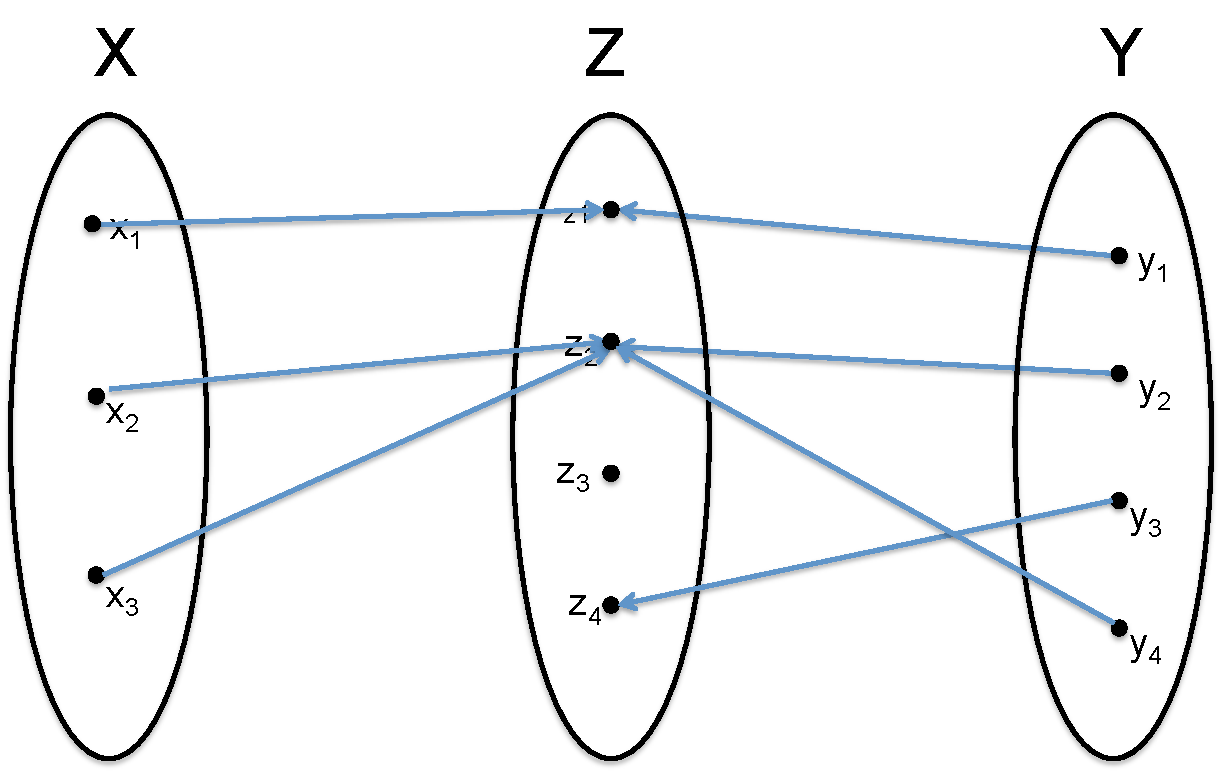
\includegraphics[height=2in]{setPullback}
\end{center}
What is the pullback of the diagram $X\Too{f}Z\Fromm{g}Y$?
\end{exerciseENG}

\begin{exerciseRUS}
Пусть $X,Y,Z$ такие, как на рисунке, а $f\taking X\to Z$ и $g\taking Y\to Z$ — изображенные функции. 
\begin{center}
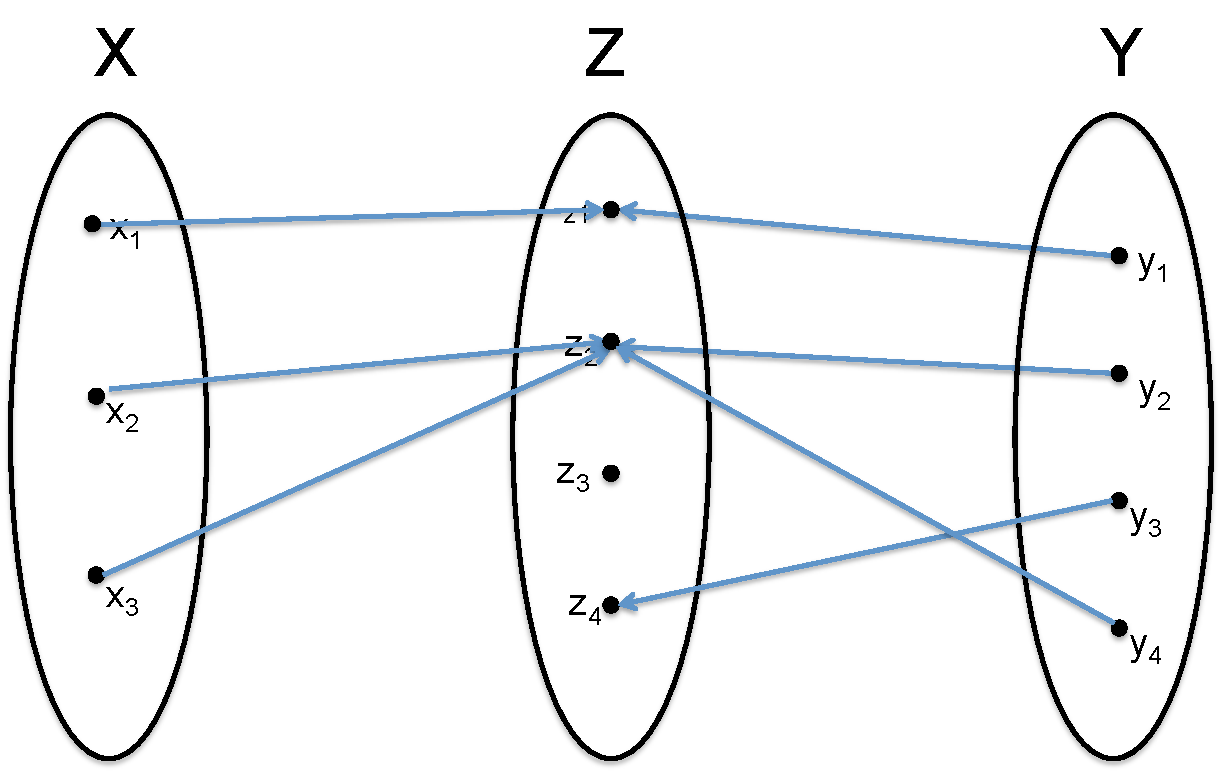
\includegraphics[height=2in]{setPullback}
\end{center}
Каким будет пулбек диаграммы $X\Too{f}Z\Fromm{g}Y$?
\end{exerciseRUS}

\begin{exerciseENG}~
\sexc Draw a set $X$ with five elements and a set $Y$ with three elements. Color each element of $X$ and each element of $Y$ either red, blue, or yellow,%
\footnote{You can use shadings rather than coloring, if coloring would be annoying.}
and do so in a “random-looking” way. Considering your coloring of $X$ as a function $X\to C$, where $C=\{\tn{red, blue, yellow}\}$, and similarly obtaining a function $Y\to C$, draw the fiber product $X\times_CY$. Make sure it is colored appropriately.
\next The universal property for products guarantees a function $X\times_CY\to X\times Y$, which I can tell you will be an injection. This means that the drawing you made of the fiber product can be imbedded into the $5\times 3$ grid; please draw the grid and indicate this subset.
\endsexc
\end{exerciseENG}

\begin{exerciseRUS}~
\sexc Нарисуйте множество $X$ из пяти элементов и множество $Y$ из трех элементов. Раскрасьте все элементы $X$ и $Y$ либо в красный, либо в синий, либо в желтый цвет,%
\footnote{Можете их заштриховать, а не раскрашивать, если раскрашивать вам неудобно.}
причем сделайте это «случайным» образом. Считая вашу раскраску $X$ функцией $X\to C$, где $C=\{\tn{красный, синий, желтый}\}$, и аналогичным образом получив функцию $Y\to C$, нарисуйте расслоенное произведение $X\times_CY$. Раскрасив его подходящим образом, убедитесь, что цвета пар совпадают.
\next Универсальное свойство произведений обеспечивает нам функцию $X\times_CY\to X\times Y$, которая, можете мне поверить, будет инъекцией. Это означает, что рисунок расслоенного произведения, который вы сделали, может быть вставлен в сетку $5\times 3$; изобразите, пожалуйста, такую сетку и отметьте на ней подмножество.
\endsexc
\end{exerciseRUS}

\begin{remarkENG}
Some may prefer to denote this fiber product by $f\times_Zg$ rather than $X\times_ZY$. The former is  mathematically better notation, but human-readability is often enhanced by the latter, which is also more common in the literature. We use whichever is more convenient.
\end{remarkENG}

\begin{remarkRUS}
Некоторые предпочитают обозначать расслоенное произведение $f\times_Zg$, а не $X\times_ZY$. Первое обозначение математически корректнее, но читабельность для человека часто лучше у второго, которое, кроме того, чаще встречается в литературе. Мы будем использовать такое обозначение, которое окажется более удобным.
\end{remarkRUS}

\begin{exerciseENG}~
\sexc Suppose that $Y=\emptyset$; what can you say about $X\times_ZY$? 
\next Suppose now that $Y$ is any set but that $Z$ has exactly one element; what can you say about $X\times_ZY$?
\endsexc
\end{exerciseENG}

\begin{exerciseRUS}~
\sexc Предположим, что $Y=\varnothing$; что вы можете сказать о $X\times_ZY$? 
\next Предположим теперь, что $Y$ — любое множество, а $Z$ имеет в точности один элемент; что вы можете сказать о $X\times_ZY$?
\endsexc
\end{exerciseRUS}

\begin{exerciseENG}
Let $S=\RR^3, T=\RR$, and think of them as (Aristotelian) space and time, with the origin in $S\times T$ given by the center of mass of MIT at the time of its founding. Let $Y=S\times T$ and let $g_1\taking Y\to S$ be one projection and $g_2\taking Y\to T$ the other projection. Let $X=\singleton$ be a set with one element and let $f_1\taking X\to S$ and $f_2\taking X\to T$ be given by the origin in both cases. 
\sexc What are the fiber products $W_1$ and $W_2$:
$$
\xymatrix{W_1\ar[r]\ar[d]\ullimit&Y\ar[d]^{g_1}\\X\ar[r]_{f_1}&S}\hspace{1in}
\xymatrix{W_2\ar[r]\ar[d]\ullimit&Y\ar[d]^{g_2}\\X\ar[r]_{f_2}&T}
$$
\next Interpret these sets in terms of the center of mass of MIT at the time of its founding.
\endsexc
\end{exerciseENG}

\begin{exerciseRUS}
Пусть $S=\RR^3, T=\RR$, будем думать о них, как об (Аристотелевых) пространстве и времени, с началом отсчета в $S\times T$, заданным центром масс [университета] MIT в момент его основания. Пусть $Y=S\times T$ и $g_1\taking Y\to S$ — одна из проекций, а $g_2\taking Y\to T$ — другая. Пусть $X=\singleton$ — множество из одного элемента, а $f_1\taking X\to S$ и $f_2\taking X\to T$ заданы как начала отсчета в обоих случаях. 
\sexc Какими будут расслоенные произведения $W_1$ и $W_2$:
$$
\xymatrix{W_1\ar[r]\ar[d]\ullimit&Y\ar[d]^{g_1}\\X\ar[r]_{f_1}&S}\hspace{1in}
\xymatrix{W_2\ar[r]\ar[d]\ullimit&Y\ar[d]^{g_2}\\X\ar[r]_{f_2}&T}
$$
\next Интерпретируйте эти множества в терминах центра масс MIT в момент его основания.
\endsexc
\end{exerciseRUS}

%% Subsubsection %%

\subsubsection{Using pullbacks to define new ideas from old / Использование пуллбеков для определения новый идей на основе старых}

In this section we will see that the fiber product of a diagram can serve to define a new concept. For example, in (\ref{dia:bad battery}) we define what it means for a cellphone to have a bad battery, in terms of the length of time for which it remains charged. By being explicit, we reduce the chance of misunderstandings between different groups of people. This can be useful in situations like audits and those in which one is trying to reuse or understand data gathered by others.

В этом разделе мы увидим, что расслоенное произведение диаграммы может послужить нам для того, чтобы определить новое понятие. Например, в (\ref{dia:bad battery}) мы определяем, что такое мобильный телефон с плохим аккумулятором, в терминах продолжительности времени, которое он остается заряженным. Выражая вещи более явно, мы уменьшаем шанс возникновения недопониманий между различными группами людей. Это может быть полезно в ситуациях вроде аудита, либо когда некто пытается использовать и понять данные, собранные другими.

\begin{exampleENG}
Consider the following two ologs. The one on the right is the pullback of the one on the left. 
\begin{align}\label{dia:wealthy and loyal}
\fbox{\xymatrixnocompile{&\obox{C}{.7in}{\rr a loyal customer}\LA{d}{is}\\\obox{B}{.7in}{\rr a wealthy customer}\LA{r}{is}&\smbox{D}{a customer}}}\hsp&\fbox{\xymatrix{\obox{A=B\times_DC}{.9in}{\rr a customer that is wealthy and loyal}\LAL{d}{is}\LA{r}{is}&\obox{C}{.7in}{\rr a loyal customer}\LA{d}{is}\\\obox{B}{.7in}{\rr a wealthy customer}\LA{r}{is}&\smbox{D}{a customer}}}
\end{align}
Check from Definition \ref{def:pullback} that the label, “a customer that is wealthy and loyal”, is fair and straightforward as a label for the fiber product $A=B\times_DC$, given the labels on $B,C$, and $D$.
\end{exampleENG}

\begin{exampleRUS}
Рассмотрим следующие два олога. Тот, что справа, является притягивающим квадратом того, что слева. 
\begin{align}\label{dia:wealthy and loyal}
\fbox{\xymatrixnocompile{&\obox{C}{.7in}{\rr покорный потребитель}\LA{d}{это}\\\obox{B}{.7in}{\rr богатый потребитель}\LA{r}{это}&\smbox{D}{потребитель}}}\hsp&\fbox{\xymatrix{\obox{A=B\times_DC}{.9in}{\rr богатый и покорный потребитель}\LAL{d}{это}\LA{r}{это}&\obox{C}{.7in}{\rr покорный потребитель}\LA{d}{это}\\\obox{B}{.7in}{\rr богатый потребитель}\LA{r}{это}&\smbox{D}{потребитель}}}
\end{align}
Проверьте по определению \ref{def:pullback}, что метка «богатый и покорный потребитель» — это корректная и достаточно прямолинейная метка для расслоенного произведения $A=B\times_DC$, если на $B,C$ и $D$ поставить соответствующие метки.%
\endnote{
С точки зрения теории множеств, мы только что построили пересечение двух подмножеств одного множества. В общем случае, такие пересечения моделируются в теории категорий именно притягивающими квадратами.
}
\end{exampleRUS}

\begin{remarkENG}\label{rem:defining using pullbacks}
Note that in Diagram (\ref{dia:wealthy and loyal}) the top-left box could have been (non-canonically named) \fakebox{a good customer}. If it was taken to be the fiber product, then the author would be effectively {\em defining} a good customer to be one that is wealthy and loyal. 
\end{remarkENG}

\begin{remarkRUS}\label{rem:defining using pullbacks}
Заметим, что в Диаграмме (\ref{dia:wealthy and loyal}) верхний левый прямоугольник может быть (неканонически) назван \fakebox{хороший потребитель}. Если указать именно его в качестве пулбека, то автор [олога] будет фактически {\em определять} хорошего потребителя как того, кто одновременно богат и покорен. 
\end{remarkRUS}

\begin{exerciseENG}
For each of the following, an author has proposed that the diagram on the right is a pullback. Do you think their labels are appropriate or misleading; that is, is the label on the upper-left box reasonable given the rest of the olog, or is it suspect in some way?
\sexc\begin{align*}\footnotesize\fbox{\xymatrix{&&\smbox{C}{blue}\LA{d}{is}\\\smbox{B}{a person}\LA{rr}{\parbox{.7in}{\rr has as favorite color}}&&\smbox{D}{a color}}}\hsp&\footnotesize\fbox{\xymatrixnocompile{\obox{A=B\times_DC}{1.1in}{\rr a person whose favorite color is blue}\LAL{d}{is}\LA{rr}{\parbox{.7in}{\rr has as favorite color}}&&\smbox{C}{blue}\LA{d}{is}\\\smbox{B}{a person}\LA{rr}{\parbox{.7in}{\rr has as favorite color}}&&\smbox{D}{a color}}}
\end{align*}
\next\begin{align*}\footnotesize\fbox{\xymatrixnocompile{&&\smbox{C}{a woman}\LA{d}{is}\\\smbox{B}{a dog}\LA{rr}{\parbox{.7in}{\rr has as owner}}&&\smbox{D}{a person}}}\hsp&\footnotesize\fbox{\xymatrixnocompile{\obox{A=B\times_DC}{1in}{\rr a dog whose owner is a woman}\LAL{d}{is}\LA{rr}{\parbox{.7in}{\rr has as owner}}&&\smbox{C}{a woman}\LA{d}{is}\\\smbox{B}{a dog}\LA{rr}{\parbox{.7in}{\rr has as owner}}&&\smbox{D}{a person}}}
\end{align*}
\next\begin{align*}\footnotesize\fbox{\xymatrixnocompile{&\obox{C}{.5in}{\rr a piece of furniture}\LA{d}{has}\\\obox{B}{.6in}{\rr a space in our house}\LA{r}{has}&\smbox{D}{a width}}}\hsp&\footnotesize\fbox{\xymatrixnocompile{\obox{A=B\times_DC}{.5in}{\rr a good fit}\LAL{d}{$s$}\LA{r}{$f$}&\obox{C}{.5in}{\rr a piece of furniture}\LA{d}{has}\\\obox{B}{.6in}{\rr a space in our house}\LA{r}{has}&\smbox{D}{a width}}}
\end{align*}
\endsexc
\end{exerciseENG}

\begin{exerciseRUS}
Для каждого из нижеследующих [ологов] автор заявляет, что диаграмма справа является притягивающим квадратом. Считаете ли вы метки подходящими или сбивающими с толку; другими словами, будет ли метка на верхнем левом прямоугольнике обоснованой остальной частью олога или же она некоторым образом вызывает подозрение?
\sexc\begin{align*}\footnotesize\fbox{\xymatrix{&&\smbox{C}{синий}\LA{d}{это}\\\smbox{B}{человек}\LA{rr}{\parbox{.7in}{\rr любимый цвет}}&&\smbox{D}{цвет}}}\hsp&\footnotesize\fbox{\xymatrixnocompile{\obox{A=B\times_DC}{1.1in}{\rr человек, который любит синий цвет}\LAL{d}{это}\LA{rr}{\parbox{.7in}{\rr любимый цвет}}&&\smbox{C}{синий}\LA{d}{это}\\\smbox{B}{человек}\LA{rr}{\parbox{.7in}{\rr любимый цвет}}&&\smbox{D}{цвет}}}
\end{align*}
\next\begin{align*}\footnotesize\fbox{\xymatrixnocompile{&&\smbox{C}{женщина}\LA{d}{это}\\\smbox{B}{собака}\LA{rr}{\parbox{.7in}{\rr владелец}}&&\smbox{D}{человек}}}\hsp&\footnotesize\fbox{\xymatrixnocompile{\obox{A=B\times_DC}{1in}{\rr собака, у которой владелец — женщина}\LAL{d}{это}\LA{rr}{\parbox{.7in}{\rr владелец}}&&\smbox{C}{женщина}\LA{d}{это}\\\smbox{B}{собака}\LA{rr}{\parbox{.7in}{\rr владелец}}&&\smbox{D}{человек}}}
\end{align*}
\next\begin{align*}\footnotesize\fbox{\xymatrixnocompile{&\obox{C}{.5in}{\rr предмет мебели}\LA{d}{имеет}\\\obox{B}{.6in}{\rr свободное место в доме}\LA{r}{имеет}&\smbox{D}{ширина}}}\hsp&\footnotesize\fbox{\xymatrixnocompile{\obox{A=B\times_DC}{.5in}{\rr подходит}\LAL{d}{$s$}\LA{r}{$f$}&\obox{C}{.5in}{\rr предмет мебели}\LA{d}{имеет}\\\obox{B}{.6in}{\rr свободное место в доме}\LA{r}{имеет}&\smbox{D}{ширина}}}
\end{align*}
\endsexc
\end{exerciseRUS}

\begin{exerciseENG}~
\sexc Consider your olog from Exercise \ref{exc:family olog}. Are any of the commutative squares there actually pullback squares? 
\next Now use ologs with products and pullbacks to define what a brother is and what a sister is (again in a human biological nuclear family), in terms of types such as \fakebox{an offspring of mating pair $(a,b)$}, \fakebox{a person}, \fakebox{a male person}, \fakebox{a female person}, and so on.
\endsexc
\end{exerciseENG}

\begin{exerciseRUS}~
\sexc Рассмотрите свой олог из Упражнения \ref{exc:family olog}. Будут ли какие-либо из коммутативных квадратов в нем притягивающими? 
\next Теперь используйте ологи с произведениями и пулбеками, чтобы определить, что такое брат, и что такое сестра (опять же, в человеческой биологической нуклеарной семье), в терминах типов, таких как \fakebox{потомок супружеской пары $(a,b)$}, \fakebox{человек}, \fakebox{мужчина}, \fakebox{женщина}, и им подобных.
\endsexc
\end{exerciseRUS}

\begin{definitionENG}[Preimage]\label{def:preimage}
Let $f\taking X\to Y$ be a function and $y\in Y$ an element. The {\em preimage of y under $f$}\index{preimage}, denoted $f^\m1(y)$,\index{a symbol!$f^\m1$} is  the subset $f^\m1(y):=\{x\in X\|f(x)=y\}$. If $Y'\ss Y$ is any subset, the {\em preimage of $Y'$ under $f$}, denoted $f^\m1(Y')$, is the subset $f^\m1(Y')=\{x\in X\|f(x)\in Y'\}$.
\end{definitionENG}

\begin{definitionRUS}[Прообраз]\label{def:preimage}
Пусть $f\taking X\to Y$ — функция и $y\in Y$ — элемент. {\em Прообраз $y$ относительно $f$}\index{прообраз}, обозначаемый $f^\m1(y)$,\index{символ!$f^\m1$} — это подмножество $f^\m1(y):=\{x\in X\|f(x)=y\}$. Если $Y'\ss Y$ — произвольное подмножество, то {\em прообраз $Y'$ относительно $f$}, обозначаемый $f^\m1(Y')$, — это подмножество $f^\m1(Y')=\{x\in X\|f(x)\in Y'\}$.
\end{definitionRUS}

\begin{exerciseENG}
Let $f\taking X\to Y$ be a function and $y\in Y$ an element. Draw a pullback diagram in which the fiber product is isomorphic to the preimage $f^\m1(y)$.
\end{exerciseENG}

\begin{exerciseRUS}
Пусть $f\taking X\to Y$ — функция и $y\in Y$ — элемент. Нарисуйте притягивающий квадрат, в котором расслоенное произведение изоморфно прообразу $f^\m1(y)$. 
\end{exerciseRUS}

\begin{lemmaENG}[Universal property for pullback]\label{lemma:up for fp}
Suppose given the diagram of sets and functions as below.
\begin{align*}
\xymatrix{&Y\ar[d]^u\\
X\ar[r]_t&Z}
\end{align*}
For any set $A$ and commutative solid arrow diagram as below (i.e. functions $f\taking A\to X$ and $g\taking A\to Y$ such that $t\circ f=u\circ g$), 
\begin{align}\label{dia:universal property of fp}
\xymatrix{
&X\times_ZY\ar@/_1pc/[lddd]_{\pi_1}\ar@/^1pc/[rddd]^{\pi_2}\\\\
&A\ar@{-->}[uu]^{\exists!}\ar[dl]_{\forall f}\ar[dr]^{\forall g}&\\
X\ar[rd]_t&&Y\ar[ld]^u\\
&Z&}
\end{align}
there exists a unique arrow $\pb{f}{g}{Z}\taking A\to X\times_ZY$ making everything commute, i.e. 
$$f=\pi_1\circ \pb{f}{g}{Z}\hsp\text{and}\hsp g=\pi_2\circ\pb{f}{g}{Z}.$$
\end{lemmaENG}

\begin{lemmaRUS}[Универсальное свойство притягивающего квадрата]\label{lemma:up for fp}
Предположим, дана следующая диаграмма множеств и функций.
\begin{align*}
\xymatrix{&Y\ar[d]^u\\
X\ar[r]_t&Z}
\end{align*}
Для любого множества $A$ и коммутативной диаграммы из непрерывных стрелок, данной ниже (т.е. функций $f\taking A\to X$ и $g\taking A\to Y$ таких, что $t\circ f=u\circ g$), 
\begin{align}\label{dia:universal property of fp}
\xymatrix{
&X\times_ZY\ar@/_1pc/[lddd]_{\pi_1}\ar@/^1pc/[rddd]^{\pi_2}\\\\
&A\ar@{-->}[uu]^{\exists!}\ar[dl]_{\forall f}\ar[dr]^{\forall g}&\\
X\ar[rd]_t&&Y\ar[ld]^u\\
&Z&}
\end{align}
существует единственная стрелка $\pb{f}{g}{Z}\taking A\to X\times_ZY$, делающая коммутативным все остальное, т.е.
$$f=\pi_1\circ \pb{f}{g}{Z}\hsp\text{and}\hsp g=\pi_2\circ\pb{f}{g}{Z}.$$
\end{lemmaRUS}

\begin{exerciseENG}
Create an olog whose underlying shape is a commutative square. Now add the fiber product so that the shape is the same as that of Diagram (\ref{dia:universal property of fp}). Assign English labels to the projections $\pi_1,\pi_2$ and to the dotted map $A\To{\pb{f}{g}{Z}}X\times_ZY$, such that these labels are as canonical as possible.
\end{exerciseENG}

\begin{exerciseRUS}
Постройте олог с произвольной коммутативной диаграммой. Теперь добавьте расслоенное произведение так, чтобы форма диаграммы стала подобной Диаграмме (\ref{dia:universal property of fp}). Дайте метки на естественном языке проекциям $\pi_1,\pi_2$ и пунктирному отображению $A\To{\pb{f}{g}{Z}}X\times_ZY$ таким образом, чтобы эти метки были по возможности каноничны.
\end{exerciseRUS}

%% Subsubsection %%

\subsubsection{Pasting diagrams for pullback / Склеивание диаграмм для пуллбеков}

Consider the diagram drawn below, which includes a left-hand square, a right-hand square, and a big rectangle.
$$
\xymatrix{
A'\ar[r]^{f'}\ar[d]_i\ullimit&B'\ar[r]^{g'}\ar[d]_j\ullimit&C'\ar[d]^k\\
A\ar[r]_f&B\ar[r]_g&C}
$$
The right-hand square has a corner symbol indicating that $B'\iso B\times_CC'$ is a pullback. But the corner symbol on the left is ambiguous; it might be indicating that the left-hand square is a pullback, or it might be indicating that the big rectangle is a pullback. It turns out that if $B'\iso B\times_CC'$ then it is not ambiguous because the left-hand square is a pullback if and only if the big rectangle is.

Рассмотрим диаграмму, изображенную ниже, которая включает коммутативные квадраты слева, справа, а также [обрамляющий их] большой прямоугольник.
$$
\xymatrix{
A'\ar[r]^{f'}\ar[d]_i\ullimit&B'\ar[r]^{g'}\ar[d]_j\ullimit&C'\ar[d]^k\\
A\ar[r]_f&B\ar[r]_g&C}
$$
Квадрат справа имеет символ-уголок, означающий, что $B'\iso B\times_CC'$ — пулбек. Но символ-уголок слева неоднозначен; он мог бы относиться и к левому квадрату, и к большому прямоугольнику. Однако оказывается, что если $B'\iso B\times_CC'$, то разночтений нет, потому что левый квадрат является притягивающим тогда и только тогда, когда таковым является большой прямоугольник.

\begin{propositionENG}\label{prop:pasting}
Consider the diagram drawn below
$$
\xymatrix{
&B'\ar[r]^{g'}\ar[d]_j\ullimit&C'\ar[d]^k\\
A\ar[r]_f&B\ar[r]_g&C}
$$
where $B'\iso B\times_CC'$ is a pullback. Then there is an isomorphism $A\times_BB'\iso A\times_CC'$. Said another way, $$A\times_B(B\times_CC')\iso A\times_CC'.$$
\end{propositionENG}

\begin{propositionRUS}\label{prop:pasting}
Рассмотрим диаграмму, изображенную ниже
$$
\xymatrix{
&B'\ar[r]^{g'}\ar[d]_j\ullimit&C'\ar[d]^k\\
A\ar[r]_f&B\ar[r]_g&C}
$$
где $B'\iso B\times_CC'$ — пулбек. Тогда имеется изоморфизм $A\times_BB'\iso A\times_CC'$. Другими словами, $$A\times_B(B\times_CC')\iso A\times_CC'.$$
\end{propositionRUS}

\begin{proofENG}
We first provide a map $\phi\taking A\times_B(B\times_CC')\to A\times_CC'$. An element of $A\times_B(B\times_CC')$ is of the form $(a,b,(b,c,c'))$ such that $f(a)=b, g(b)=c$ and $k(c')=c$. But this implies that $g\circ f(a)=c=k(c')$ so we put $\phi(a,b,(b,c,c')):=(a,c,c')\in A\times_CC'$. Now we provide a proposed inverse, $\psi\taking A\times_CC'\to A\times_B(B\times_CC')$. Given $(a,c,c')$ with $g\circ f(a)=c=k(c')$, let $b=f(a)$ and note that $(b,c,c')$ is an element of $B\times_CC'$. So we can define $\psi(a,c,c')=(a,b,(b,c,c'))$. It is easy to see that $\phi$ and $\psi$ are inverse.
\end{proofENG}

\begin{proofRUS}
Сначала получим отображение $\phi\taking A\times_B(B\times_CC')\to A\times_CC'$. Элементы из $A\times_B(B\times_CC')$ имеют вид $(a,b,(b,c,c'))$ таких, что $f(a)=b, g(b)=c$ и $k(c')=c$. Но из этого следует, что $g\circ f(a)=c=k(c')$, так что мы можем положить $\phi(a,b,(b,c,c')):=(a,c,c')\in A\times_CC'$. Теперь получим необходимое обратное отображение $\psi\taking A\times_CC'\to A\times_B(B\times_CC')$. Для данного $(a,c,c')$ с $g\circ f(a)=c=k(c')$, пусть $b=f(a)$; заметим, что $(b,c,c')$ — элемент $B\times_CC'$. Поэтому мы можем определить $\psi(a,c,c')=(a,b,(b,c,c'))$. Легко видеть, что $\phi$ и $\psi$ будут взаимно обратными.
\end{proofRUS}

Proposition \ref{prop:pasting} can be useful in authoring ologs. For example, the type \fakebox{a cellphone that has a bad battery} is vague, but we can lay out precisely what it means using pullbacks:
\small
\begin{align}\label{dia:bad battery}
\fbox{\xymatrixnocompile{\obox{A\iso B\times_DC}{1in}{a cellphone that has a bad battery}\ar[r]\ar[d]&\smbox{C\iso D\times_FE}{a bad battery}\ar[r]\ar[d]&\obox{E\iso F\times_HG}{.5in}{less than 1 hour}\ar[r]\ar[d]&\obox{G}{.5in}{between 0 and 1}\ar[d]\\\smbox{B}{a cellphone}\LA{r}{has}&\smbox{D}{a battery}\LA{r}{\parbox{.4in}{\rr remains charged for}}&\obox{F}{.6in}{a duration of time}\LA{r}{\hspace{.07in}\parbox{.4in}{\rr in hours yields}}&\obox{H}{.6in}{a range of numbers}}}
\end{align}\normalsize

Утверждение \ref{prop:pasting} может оказаться полезным при создании ологов. Например, тип \fakebox{мобильный телефон с плохим аккумулятором} определен туманно, но мы можем точно сформулировать, что оно означает, используя пулбеки:
\small
\begin{align}\label{dia:bad battery}
\fbox{\xymatrixnocompile{\obox{A\iso B\times_DC}{1in}{мобильный телефон с плохим аккумулятором}\ar[r]\ar[d]&\smbox{C\iso D\times_FE}{плохой аккумулятор}\ar[r]\ar[d]&\obox{E\iso F\times_HG}{.5in}{менее 1 часа}\ar[r]\ar[d]&\obox{G}{.5in}{между 0 и 1}\ar[d]\\\smbox{B}{мобильный телефон}\LA{r}{имеет}&\smbox{D}{аккумулятор}\LA{r}{\parbox{.4in}{\rr остается заряженным}}&\obox{F}{.6in}{промежуток времени}\LA{r}{\hspace{.07in}\parbox{.4in}{\rr в часах}}&\obox{H}{.6in}{числовой промежуток}}}
\end{align}\normalsize

The category-theoretic fact described above says that since $A\iso B\times_DC$ and $C\iso D\times_FE$, it follows that $A\iso B\times_FE$.  That is, we can deduce the definition “a cellphone that has a bad battery is defined as a cellphone that has a battery which remains charged for less than one hour.”  

Теоретико-категорный факт, описанный выше, говорит, что из $A\iso B\times_DC$ и $C\iso D\times_FE$ следует $A\iso B\times_FE$. Это значит, мы можем вывести такое определение «мобильный телефон с плохим аккумулятором определяется как мобильный телефон, имеющий аккумулятор, который остается заряженным менее одного часа.»

\begin{exerciseENG}~
\sexc Create an olog that defines two people to be “of approximately the same height” if and only if their height difference is less than half an inch, using a pullback. Your olog can include the box \fakebox{a real number $x$ such that $-.5<x<.5$}. 
\next In the same olog, make a box for those people whose height is approximately the same as a person named “The Virgin Mary”. You may need to use images, as in Section \ref{sec:images}.
\endsexc
\end{exerciseENG}

\begin{exerciseRUS}~
\sexc Придумать олог, который при помощи пулбека определяет, что два человека «имеют приблизительно однаковый рост», если и только если разность их роста меньше половины дюйма. Ваш олог может включать прямоугольник \fakebox{действительное число $x$ такое, что $-.5<x<.5$}. 
\next В тот же олог добавьте прямоугольник для людей, чей рост приблизительно совпадает с ростом человека по имени «Дева Мария». Вам могут потребоваться образы функций, см. Раздел \ref{sec:images}.
\endsexc
\end{exerciseRUS}

\begin{exerciseENG}\label{exc:pointwise map of fp}
Consider the diagram on the left below, where both squares commute. 
$$
\xymatrix@=15pt{
&&&Y'\ar[dd]\\
&&Y\ar[ru]\ar[dd]\\
&X'\ar'[r][rr]&&Z'\\
X\ar[rr]\ar[ru]&&Z\ar[ru]
}
\hspace{1in}
\xymatrix@=15pt{
&W'\ar[rr]\ar'[d][dd]\ullimit&&Y'\ar[dd]\\
W\ar[rr]\ar[dd]\ullimit&&Y\ar[ru]\ar[dd]\\
&X'\ar'[r][rr]&&Z'\\
X\ar[rr]\ar[ru]&&Z\ar[ru]
}
$$
Let $W=X\times_ZY$ and $W'=X'\times_{Z'}Y'$, and form the diagram to the right. Use the universal property of fiber products to construct a map $W\to W'$ such that all squares commute.
\end{exerciseENG}

\begin{exerciseRUS}\label{exc:pointwise map of fp}
Рассмотрим следующую диаграмму слева, в которой оба квадрата коммутируют: 
$$
\xymatrix@=15pt{
&&&Y'\ar[dd]\\
&&Y\ar[ru]\ar[dd]\\
&X'\ar'[r][rr]&&Z'\\
X\ar[rr]\ar[ru]&&Z\ar[ru]
}
\hspace{1in}
\xymatrix@=15pt{
&W'\ar[rr]\ar'[d][dd]\ullimit&&Y'\ar[dd]\\
W\ar[rr]\ar[dd]\ullimit&&Y\ar[ru]\ar[dd]\\
&X'\ar'[r][rr]&&Z'\\
X\ar[rr]\ar[ru]&&Z\ar[ru]
}
$$
Положив $W=X\times_ZY$ и $W'=X'\times_{Z'}Y'$, образуем диаграмму справа. Используя универсальное свойство расслоенных произведений, сконструируйте отображение $W\to W'$ такое, чтобы все квадраты коммутировали.
\end{exerciseRUS}

%%%% Subsection %%%%

\subsection{Spans, experiments, and matrices / Развилки, эксперименты и матрицы}

\begin{definitionENG}\label{def:span}\index{span}
Given sets $A$ and $B$, a {\em span on $A$ and $B$} is a set $R$ together with functions $f\taking R\to A$ and $g\taking R\to B$. 
$$\xymatrix@=15pt{&R\ar[ddl]_f\ar[ddr]^g\\\\A&&B}$$
\end{definitionENG}

\begin{definitionRUS}\label{def:span}\index{спан}\index{развилка}
Для данных множеств $A$ и $B$ {\em развилка} между $A$ и $B$ (иногда говорят {\em спан}) это множество $R$ вместе с функциями $f\taking R\to A$ и $g\taking R\to B$. 
$$\xymatrix@=15pt{&R\ar[ddl]_f\ar[ddr]^g\\\\A&&B}$$
\end{definitionRUS}

\begin{applicationENG}\label{app:exp temp press}
Think of $A$ and $B$ as observables and $R$ as a set of experiments performed on these two variables. For example, let's say $T$ is the set of possible temperatures of a \href{http://en.wikipedia.org/wiki/Ideal_gas_law}{\text gas} in a fixed container and let's say $P$ is the set of possible pressures of the gas. We perform 1000 experiments in which we change and record the temperature and we simultaneously also record the pressure; this is a span $T\From{f}E\To{g}P$. The results might look like this:
$$
\begin{tabular}{| l || l | l |}
\bhline
\multicolumn{3}{| c |}{Experiment}\\\bhline
{\bf ID}&{\bf Temperature}&{\bf Pressure}\\\bbhline
1&100& 72\\\hline
2&100&73\\\hline
3&100&72\\\hline
4&200&140\\\hline
5&200&138\\\hline
6&200&141\\\hline
\vdots&\vdots&\vdots\\\bhline
\end{tabular}
$$
\end{applicationENG}

\begin{applicationRUS}\label{app:exp temp press}
Думайте об $A$ и $B$, как о наблюдаемых величинах, и об $R$ как о множестве экспериментов, производимых, чтобы получить эти величины. Например, положим $T$ — множество возможных температур \href{http://en.wikipedia.org/wiki/Ideal_gas_law}{\text идеального газа} в жестком контейнере, а $P$ — множество возможных давлений этого газа. Произведем $1000$ экспериментов, в которых мы изменяем и записываем температуру и одновременно давление; это развилка $T\From{f}E\To{g}P$. Результат может выглядеть так:
$$
\begin{tabular}{| l || l | l |}
\bhline
\multicolumn{3}{| c |}{эксперимент}\\\bhline
{\bf №}&{\bf температура}&{\bf давление}\\\bbhline
1&100& 72\\\hline
2&100&73\\\hline
3&100&72\\\hline
4&200&140\\\hline
5&200&138\\\hline
6&200&141\\\hline
\vdots&\vdots&\vdots\\\bhline
\end{tabular}
$$
\end{applicationRUS}

\begin{definitionENG}\label{def:composite span}
Let $A,B,$ and $C$ be sets, and let $A\From{f}R\To{g}B$ and $B\From{f'}R'\To{g'}C$ be spans. Their {\em composite span}\index{span!composite} is given by the fiber product $R\times_BR'$ as in the diagram below:
$$
\xymatrix@=10pt{&&R\times_BR'\ar[ldd]\ar[rdd]\\\\&R\ar[ddl]_f\ar[ddr]^g&&R'\ar[ddl]_{f'}\ar[ddr]^{g'}\\\\A&&B&&C
}$$
\end{definitionENG}

\begin{definitionRUS}\label{def:composite span}
Пусть $A,B$ и $C$ — множества, а $A\From{f}R\To{g}B$ и $B\From{f'}R'\To{g'}C$ — развилки. Их {\em композиция}\index{развилка!композиция} задается таким расслоенным произведением $R\times_BR'$, как на диаграмме ниже:
$$
\xymatrix@=10pt{&&R\times_BR'\ar[ldd]\ar[rdd]\\\\&R\ar[ddl]_f\ar[ddr]^g&&R'\ar[ddl]_{f'}\ar[ddr]^{g'}\\\\A&&B&&C
}$$
\end{definitionRUS}

\begin{applicationENG}\label{app:exp temp press 2}
Let's look back at our lab's experiment from Application \ref{app:exp temp press}, which resulted in a span $T\From{f}E\To{g}P$. Suppose we notice that something looks a little wrong. The pressure should be linear in the temperature but it doesn't appear to be. We hypothesize that the volume of the container is increasing under pressure. We look up this container online and see that experiments have been done to measure the volume as the interior pressure changes. The data has generously been made available online, which gives us a span $P\From{f'}E'\To{g'}V$. 

The composite of our lab's span with the online data span yields a span $T\from E''\to V$, where $E'':=E\times_PE'$. What information does this span give us? In explaining it, one might say “whenever an experiment in our lab yielded the same pressure as one they recorded, let's call that a data point. Every data point has an associated temperature (from our lab) and an associated volume (from their experiment). This is the best we can do.” 

The information we get this way might be seen by some as unscientific, but it certainly is the kind of information people use in business and in every day life calculation — we get our data from multiple sources and put it together. Moreover, it is scientific in the sense that it is reproducible. The way we obtained our $T$-$V$ data is completely transparent.
\end{applicationENG}

\begin{applicationRUS}\label{app:exp temp press 2}
Давайте вернемся к нашему эксперименту из Прикладного примера \ref{app:exp temp press}, результат которого представим в виде развилки $T\From{f}E\To{g}P$. Предположим, мы обнаружили, будто нечто пошло неправильно. Давление должно зависеть линейно от температуры, но обнаружилось, что это не так. Мы можем высказать гипотезу, что объем контейнера растет с давлением. Мы ищем данные об этом контейнере в интернет и обнаруживаем, что уже были проделаны эксперименты по измерению объема этого контейнера при изменении давления. Данные были великодушно выложены в свободный доступ, что дает нам развилку $P\From{f'}E'\To{g'}V$. 

При помощи композиции нашей лабораторной развилки и развилки с данными из интернет получим новую развилку $T\from E''\to V$, где $E'':=E\times_PE'$. Какую информацию эта развилка дает нам? Для объяснения этого можно сказать «каждый раз, когда эксперимент в нашей латоратории выдает такое давление, какое мы записали, назовем это измерительной точкой. Каждая измерительная точка имеет связанную с ней температуру (из нашей лаборатории) и объем (из чужого эксперимента). Это лучшее из того, что можно получить.»

Информация, которую мы получим таким способом может показаться в чем-то ненаучной, но это именно тот вид информации, которую люди используют в бизнесе и в ежедневных бытовых вычислениях: мы получаем данные из многих источников и соединяем их вместе. Более того, этот способ научен в том смысле, что он воспроизводим. Способ, которым мы получили наши данные о зависимости $T$-$V$ совершенно прозрачен.
\end{applicationRUS}

We can relate spans to matrices of natural numbers, and see a natural “categorification” of matrix addition and matrix multiplication. If our spans come from experiments as in Applications \ref{app:exp temp press} and \ref{app:exp temp press 2} the matrices involved will look like huge but sparse matrices. Let's go through that.

Можно найти связи развилок и матриц из натуральных чисел и получить естественную «категорификацию» матричных сложения и умножения. Если взять наши развилки, полученные в экспериментах из Прикладных примеров \ref{app:exp temp press} и \ref{app:exp temp press 2}, то соответствующие матрицы будут огромными и разреженными. Изложим это подробнее.

Let $A$ and $B$ be sets and let $A\from R\to B$ be a span. By the universal property of products, we have a unique map $R\To{p}A\times B$. 

Пусть $A$ и $B$ — множества, а $A\from R\to B$ — развилка. Согласно универсальному свойству произведений у нас имеется единственное отображение $R\To{p}A\times B$. 

We make a matrix of natural numbers out of this data as follows. The set of rows is $A$, the set of columns is $B$. For elements $a\in A$ and $b\in B$, the $(a,b)$-entry is the cardinality of its preimage, $|p^\m1(a,b)|$, i.e. the number of elements in $R$ that are sent by $p$ to $(a,b)$. 

Построим матрицу из натуральных чисел следующим образом. В качестве множества строк возьмем $A$, множества столбцов — $B$. Для элементов $a\in A$ и $b\in B$ ячейка $(a,b)$ будет содержать мощность прообраза $|p^\m1(a,b)|$, т.е. число элементов $R$ переходящих в $(a,b)$ при помощи $p$. 

Suppose we are given two $(A,B)$-spans, i.e. $A\from R\to B$ and $A\from R'\to B$; we might think of these has having the same {\em dimensions}, i.e. they are both $|A|\times|B|$-matrices. We can take the disjoint union $R\sqcup R'$ and by the universal property of coproducts we have a unique span $A\from R\sqcup R'\to B$ making the requisite diagram commute.%
\footnote{
$$\xymatrix{
&R\ar[dl]\ar[dr]\ar[d]\\
A&R\sqcup R'\ar[l]\ar[r]&B\\
&R'\ar[ur]\ar[ul]\ar[u]}
$$
}
The matrix corresponding to this new span will be the sum of the matrices corresponding to the two previous spans out of which it was made.

Предположим, даны две $(A,B)$-развилки, например $A\from R\to B$ и $A\from R'\to B$; о них можно думать, как об имеющих общую {\em размерность}, другими словами обе являются $|A|\times|B|$-матрицами. Мы можем взять несвязное объединение $R\sqcup R'$ и из универсального свойства копроизведений получить единственную развилку $A\from R\sqcup R'\to B$, делающую необходимую нам диаграмму коммутирующей.%
\footnote{
$$\xymatrix{
&R\ar[dl]\ar[dr]\ar[d]\\
A&R\sqcup R'\ar[l]\ar[r]&B\\
&R'\ar[ur]\ar[ul]\ar[u]}
$$
}
Матрица, соответствующая этой новой развилке, будет суммой матриц, соответствующих развилкам, из которых мы ее получили.

Given a span $A\from R\to B$ and a span $B\from S\to C$, the composite span can be formed as in Definition \ref{def:composite span}. It will correspond to the usual multiplication of matrices.

Для данных развилок $A\from R\to B$ и $B\from S\to C$ можно образовать их композицию (см. Определение \ref{def:composite span}). Она будет соответствовать обычному умножению матриц.

\begin{constructionENG}\label{const:bipartite}\index{graph!bipartite}
Given a span $A\From{f} R\To{g} B$, one can draw a {\em bipartite graph} with each element of $A$ drawn as a dot on the left, each element of $B$ drawn as a dot on the right, and each element $r\in R$ drawn as an arrow connecting vertex $f(r)$ on the left to vertex $g(r)$ on the right.
\end{constructionENG}

\begin{constructionRUS}\label{const:bipartite}\index{граф!двудольный}
Для данной развилки $A\From{f} R\To{g} B$ можно изобразить {\em двудольный граф}, где каждый элемент $A$ представлен вершиной слева, кадый элемент $B$ — вершиной справа, а каждый элемент $r\in R$ — стрелкой, связывающей вершину $f(r)$ слева с вершиной $g(r)$ справа.
\end{constructionRUS}

\begin{exerciseENG}~
\sexc Draw the bipartite graph (as in Construction \ref{const:bipartite}) corresponding to the span $T\From{f}E\To{g}P$ in Application \ref{app:exp temp press}.
\next Now make up your own span $P\From{f'}E'\To{g'}V$ and draw it. Finally, draw the composite span below. 
\next Can you say how the composite span graph relates to the graphs of its factors?
\endsexc
\end{exerciseENG}

\begin{exerciseRUS}~
\sexc Нарисуйте двудольный граф (как в Конструкции \ref{const:bipartite}), соответствующий развилке $T\From{f}E\To{g}P$ в Прикладном примере \ref{app:exp temp press}.
\next Теперь придумайте свою собственную развилку $P\From{f'}E'\To{g'}V$ и нарисуйте ее. Наконец, нарисуйте ниже композицию [этих двух развилок]. 
\next Сможете ли вы объяснить, как связан граф композиции развилок с графами ее сомножителей?
\endsexc
\end{exerciseRUS}

%%%% Subsection %%%%

\subsection{Equalizers and terminal objects / Уравнители и терминальные объекты}

\begin{definitionENG}\label{def:equalizer}\index{equalizer}
Suppose given two parallel arrows 
\begin{align}\label{dia:equalizer}
\xymatrix{X\ar@<.5ex>[r]^f\ar@<-.5ex>[r]_g&Y.}\hspace{1in}\xymatrix{Eq(f,g)\ar[r]^-p&X\ar@<.5ex>[r]^f\ar@<-.5ex>[r]_g&Y}
\end{align}
The {\em equalizer of $f$ and $g$} is the commutative diagram as to the right in (\ref{dia:equalizer}), where we define $$Eq(f,g):=\{x\in X\|f(x)=g(x)\}$$ and where $p$ is the canonical inclusion.
\end{definitionENG}

\begin{definitionRUS}\label{def:equalizer}\index{уравнитель}
Предположим, даны две параллельные стрелки
\begin{align}\label{dia:equalizer}
\xymatrix{X\ar@<.5ex>[r]^f\ar@<-.5ex>[r]_g&Y.}\hspace{1in}\xymatrix{Eq(f,g)\ar[r]^-p&X\ar@<.5ex>[r]^f\ar@<-.5ex>[r]_g&Y}
\end{align}
{\em Уравнитель $f$ и $g$} — это коммутативная диаграмма справа (\ref{dia:equalizer}), где мы определяем $$Eq(f,g):=\{x\in X\|f(x)=g(x)\},$$ и где  $p$ — каноническое вложение.
\end{definitionRUS}

\begin{exampleENG}
Suppose one has designed an experiment to test a theoretical prediction. The question becomes, “when does the theory match the experiment?” The answer is given by the equalizer of the following diagram:
$$\xymatrix{
\obox{}{.5in}{an input}\ar@<1ex>[rr]^{\tn{should, according to theory, yield}}\ar@<-1ex>[rr]_{\tn{according to experiment yields}}&\hspace{1in}&\obox{}{.6in}{an output}
}$$
The equalizer is the set of all inputs for which the theory and the experiment yield the same output.
\end{exampleENG}

\begin{exampleRUS}
Предположим, для проверки теоретического предсказания разработан определенный эксперимент. Возникает вопрос, «когда теория соответствует эксперименту?» Ответ дается уравнителем следующей диаграммы:
$$\xymatrix{
\obox{}{.5in}{an input}\ar@<1ex>[rr]^{\tn{should, according to theory, yield}}\ar@<-1ex>[rr]_{\tn{according to experiment yields}}&\hspace{1in}&\obox{}{.6in}{an output}
}$$
В данном случае уравнитель — это множество всех исходных условий, для которых теория и эксперимент дают одинаковый результат.
\end{exampleRUS}

\begin{exerciseENG}
Come up with an olog that uses equalizers in a reasonably interesting way. Alternatively, use an equalizer to specify those published authors who have published exactly one paper. Hint: find a function from authors to papers; then find another.
\end{exerciseENG}

\begin{exerciseRUS}
Предложите олог, использующий уравнители достаточно интересным способом. Либо используйте уравнитель, чтобы определить тех опубликованных авторов, что опубликовали ровно одну статью. Подсказка: опишите функцию из авторов в статьи; потом опишите другую функцию.
\end{exerciseRUS}

\begin{exerciseENG}
Find a universal property enjoyed by the equalizer of two arrows, and present it in the style of Lemmas \ref{lemma:up for prod}, \ref{lemma:up for coprod}, and \ref{lemma:up for fp}.
\end{exerciseENG}

\begin{exerciseRUS}
Придумайте универсальное свойство, которым обладает уравнитель двух стрелок, и запишите его аналогично Леммам \ref{lemma:up for prod}, \ref{lemma:up for coprod}, и \ref{lemma:up for fp}.
\end{exerciseRUS}

\begin{exerciseENG}\index{terminal object!in $\Set$}~
\sexc A terminal set is a set $S$ such that for every set $X$, there exists a unique function $X\to S$. Find a terminal set. 
\next Do you think that the notion {\em terminal set} belongs in this section (Section \ref{sec:finite limits})? How so? If products, pullbacks, and equalizers are all limits, what do limits have in common?
\endsexc
\end{exerciseENG}

\begin{exerciseRUS}\index{terminal object!in $\Set$}~
\sexc Терминальное множество — это множество $S$ такое, что для любого множества $X$ существует единственная функция $X\to S$. Найдите хотя бы одно терминальное множество. 
\next Как вы считаете, принадлежит ли понятие {\em терминального множества} данному разделу (Раздел \ref{sec:finite limits})? Почему? Если все — произведения, пулбеки и уравнители — являются пределами, то что общего у всех пределов?
\endsexc
\end{exerciseRUS}

%%%%%% Section %%%%%%

\section{Finite colimits in $\Set$ / Конечные копределы в $\Set$}\label{sec:finite colimits}

This section will parallel Section \ref{sec:finite limits} — I will introduce several types of finite colimits and hope that this gives the reader some intuition about them, without formally defining them yet. Before doing so, I must define equivalence relations and quotients.

Этот раздел воспроизводит структуру Раздела \ref{sec:finite limits} — я ввожу несколько видов конечных копределов в надежде, что это даст читателю интуитивное представление о них, без необходимости их пока формально определять. Однако прежде я введу отношения эквивалентности и фактор-множества.

%%%% Subsection %%%%

\subsection{Background: equivalence relations / Отступление: отношения эквивалентности}\index{equivalence relation}\index{relation!equivalence}\index{отношение!эквивалентности}

\begin{definitionENG}[Equivalence relations and equivalence classes]
Let $X$ be a set. An {\em equivalence relation on $X$} is a subset $R\ss X\times X$ satisfying the following properties for all $x,y,z\in X$:
\begin{description}
\item[Reflexivity:] $(x,x)\in R$;
\item[Symmetry:] $(x,y)\in R$ if and only if $(y,x)\in R$; and
\item[Transitivity:] if $(x,y)\in R$ and $(y,z)\in R$ then $(x,z)\in R$.
\end{description}
If $R$ is an equivalence relation, we often write $x\sim_R y$, or simply $x\sim y$, to mean $(x,y)\in R$. For convenience we may refer to the equivalence relation by the symbol $\sim$, saying that $\sim$ is an equivalence relation on $X$.\index{a symbol!$\sim$}

An {\em equivalence class of $\sim$}\index{equivalence relation!equivalence classes} is a subset $A\ss X$ such that
\begin{itemize}
\item $A$ is nonempty, $A\neq\emptyset$;
\item if $x\in A$ and $x'\in A$, then $x\sim x'$; and 
\item if $x\in A$ and $x\sim y$, then $y\in A$.
\end{itemize}
Suppose that $\sim$ is an equivalence relation on $X$. The {\em quotient of $X$ by $\sim$}\index{equivalence relation!quotient by}, denoted $X/\sim$\index{a symbol!$X/\sim$} is the set of equivalence classes of $\sim$.
\end{definitionENG}

\begin{definitionRUS}[Отношения эквивалентности и классы эквивалентности]
Пусть $X$ — множество. {\em Отношение эквивалентности на $X$} — это подмножество $R\ss X\times X$, удовлетворяющее следующим условиям для всех $x,y,z\in X$:
\begin{description}
\item[Рефлексивность:] $(x,x)\in R$;
\item[Симметричность:] $(x,y)\in R$ если и только если $(y,x)\in R$; и
\item[Транзитивность:] если $(x,y)\in R$ и $(y,z)\in R$, то $(x,z)\in R$.
\end{description}
Если $R$ — отношение эквивалентности, это часто обозначается $x\sim_R y$ или $x\sim y$, имея в виду $(x,y)\in R$. Для удобства мы, говоря о самом отношении эквивалентности $R$ над $X$, будем обозначать его символом $\sim$.\index{символ!$\sim$}

{\em Классом эквивалентности}\index{equivalence relation!equivalence classes} для $\sim$ называется подмножество $A\ss X$ такое, что
\begin{itemize}
\item $A$ не является пустым, $A\neq\emptyset$;
\item если $x\in A$ и $x'\in A$, то $x\sim x'$; и 
\item если $x\in A$ и $x\sim y$, то $y\in A$.
\end{itemize}
Предположим, что $\sim$ — отношение эквивалентности на $X$. Тогда множество всех классов эквивалентности для $\sim$ называется {\em фактор-множеством $X$ по эквивалентности $\sim$}\index{отношение!эквивалентности!фактор-множество}, обозначаемым $X/\sim$\index{символ!$X/\sim$}.
\end{definitionRUS}

\begin{exampleENG}
Let $\ZZ$ denote the set of integers. Define a relation $R\ss\ZZ\times\ZZ$ by $$R=\{(x,y)\|\exists n\in\ZZ \tn{ such that } x+7n=y\}.$$ Then $R$ is an equivalence relation because $x+7*0=x$ (reflexivity); $x+7*n=y$ if and only if $y+7*(-n)= x$ (symmetry); and $x+7n=y$ and $y+7m=z$ together imply that $x+7(m+n)=z$ (transitivity).
\end{exampleENG}

\begin{exampleRUS}
Пусть $\ZZ$ обозначает множество целых чисел. Определим отношение $R\ss\ZZ\times\ZZ$ таким образом: $$R=\{(x,y)\|\exists n\in\ZZ \tn{ такое, что } x+7n=y\}.$$ Тогда $R$ является отношением эквивалентности, поскольку $x+7*0=x$ (рефлексивность); $x+7*n=y$ если и только если $y+7*(-n)= x$ (симметричность); наконец, из $x+7n=y$ и $y+7m=z$ одновременно следует, что $x+7(m+n)=z$ (транзитивность).
\end{exampleRUS}

\begin{exerciseENG}
Let $X$ be the set of people on earth; define a binary relation $R\ss X\times X$ on $X$ as follows. For a pair $(x,y)$ of people, say $(x,y)\in R$ if $x$ spends a lot of time thinking about $y$. 
\sexc Is this relation reflexive? 
\next Is it symmetric? 
\next Is it transitive?
\endsexc
\end{exerciseENG}

\begin{exerciseRUS}
Пусть $X$ — множество людей на земле; определим бинарное отношение $R\ss X\times X$ на $X$ следующим образом. Для пары людей $(x,y)$ будем считать, что $(x,y)\in R$, если $x$ проводит много времени, думая об $y$. 
\sexc Будет ли это отношение рефлексивным? 
\next Будет ли оно симметричным? 
\next Будет ли оно транзитивным?
\endsexc
\end{exerciseRUS}

\begin{exampleENG}[Partitions]\label{ex:partition}
An equivalence relation on a set $X$ can be thought of as a way of partitioning $X$. A {\em partition of $X$}\index{equivalence relation!as partition} consists of a set $I$, called {\em the set of parts}, and for every element $i\in I$ a subset $X_i\ss X$ such that two properties hold:
\begin{itemize}
\item every element $x\in X$ is in some part (i.e. for all $x\in X$ there exists $i\in I$ such that $x\in X_i$); and
\item no element can be found in two different parts (i.e. if $x\in X_i$ and $x\in X_j$ then $i=j$).
\end{itemize}

Given a partition of $X$, we define an equivalence relation $\sim$ on $X$ by saying $x\sim x'$ if $x$ and $x'$ are in the same part (i.e. if there exists $i\in I$ such that $x,x'\in X_i$). The parts become the equivalence classes of this relation. Conversely, given an equivalence relation, one makes a partition on $X$ by taking $I$ to be the set of equivalence classes and for each $i\in I$ letting $X_i$ be the elements in that equivalence class.
\end{exampleENG}

\begin{exampleRUS}[Разбиения]\label{ex:partition}
Об отношении эквивалентности на множестве $X$ можно думать, как о способе разбить $X$ на части. {\em Разбиение $X$}\index{отношение!эквивалентности!как разбиение} состоит из множества $I$, называемого {\em множеством частей}, и для каждого элемента $i\in I$ — подмножества $X_i\ss X$ такого, что выполняются два условия:
\begin{itemize}
\item каждый элемент $x\in X$ находится в некоторой части (то есть, для всех $x\in X$ существует $i\in I$ такой, что $x\in X_i$); и
\item ни один элемент не находится в двух различных частях (то есть, если $x\in X_i$ и $x\in X_j$, то $i=j$).
\end{itemize}

Для данного рабиения $X$ определим отношение эквивалентности $\sim$ на $X$, положив $x\sim x'$, если $x$ и $x'$ находятся в одной и той же части (то есть, если существует $i\in I$ такой, что $x,x'\in X_i$). Части оказываются классами эквивалентности этого отношения. Обратно, для данного отношения эквивалентности построим разбиение $X$, взяв в качестве $I$ множество классов эквивалентности и для каждого $i\in I$ положив, что $X_i$ состоит из элементов этого класса.
\end{exampleRUS}

\begin{exerciseENG}
Let $X$ and $B$ be sets and let $f\taking X\to B$ be a function. Define a subset $R\ss X\times X$ by $$R=\{(x,y)\|f(x)=f(y)\}.$$ 
\sexc Is $R$ an equivalence relation? 
\next Are all equivalence relations on $X$ obtainable in this way (as the fibers of some function having domain $X$)?
\next Does this viewpoint on equivalence classes relate to that of Example \ref{ex:partition}?
\endsexc
\end{exerciseENG}

\begin{exerciseRUS}
Пусть $X$ и $B$ — это множество, а $f\taking X\to B$ — функция. Определим подмножество $R\ss X\times X$ как $$R=\{(x,y)\|f(x)=f(y)\}.$$ 
\sexc Будет ли $R$ отношением эквивалентности? 
\next Можно ли все отношения эквивалентности на $X$ получить таким же способом (как «слои» некоторой функции с областью определения $X$)?
\next Связана ли эта точка зрения на классы эквивалентности с Примером \ref{ex:partition}?
\endsexc
\end{exerciseRUS}

\begin{exerciseENG}
Take a set $I$ of sets; i.e. suppose that for each element $i\in I$ you are given a set $X_i$. For every two elements $i,j\in I$ say that $i\sim j$ if $X_i$ and $X_j$ are isomorphic. Is this relation an equivalence relation on $I$?  
\end{exerciseENG}

\begin{exerciseRUS}
Возьмем множество $I$ некоторых множеств; то есть предположим, что для каждого элемента $i\in I$ задано множество $X_i$. Для каждых двух элементов $i,j\in I$ будем считать, что $i\sim j$, если $X_i$ и $X_j$ изоморфны. Будет ли это отношение отношением эквивалентности на $I$?
\end{exerciseRUS}

\begin{lemmaENG}[Generating equivalence relations]\label{lemma:generating ERs}
Let $X$ be a set and $R\ss X\times X$ a subset. There exists a relation $S\ss X\times X$ such that
\begin{itemize}
\item $S$ is an equivalence relation,
\item $R\ss S$, and
\item for any equivalence relation $S'$ such that $R\ss S'$, we have $S\ss S'$.
\end{itemize}
The relation $S'$ will be called {\em the equivalence relation generated by $R$}.\index{equivalence relation!generated}
\end{lemmaENG}

\begin{lemmaRUS}[Порождение отношений эквивалентности]\label{lemma:generating ERs}
Пусть $X$ — это множество, а $R\ss X\times X$ — подмножество. Существует отношение $S\ss X\times X$ такое, что
\begin{itemize}
\item $S$ является отношением эквивалентности,
\item $R\ss S$, и
\item для любого отношения эквивалентности $S'$ такого, что $R\ss S'$, выполняется $S\ss S'$.
\end{itemize}
Отношение $S'$ назовем {\em отношением эквивалентности, порожденным $R$}.\index{отношение!эквивалентности!порожденное}
\end{lemmaRUS}

\begin{proofENG}
Let $L_R$ be the set of all equivalence relations on $X$ that contain $R$; in other words, each element $\ell\in L_R$ is an equivalence relation, $\ell\in X\times X$. The set $L_R$ is non-empty because $X\times X\ss X\times X$ is an equivalence relation. Let $S$ denote the set of pairs $(x_1,x_2)\in X\times X$ that appear in every element of $L_R$. Note that $R\ss S$ by definition. We need only show that $S$ is an equivalence relation.

It is clearly reflexive, because $R$ is. If $(x,y)\in S$ then $(x,y)\in\ell$ for all $\ell\in L_R$. But since each $\ell$ is an equivalence relation, $(y,x)\in\ell$ too, so $(y,x)\in S$. This shows that $S$ is symmetric. The proof that it is transitive is similar: if $(x,y)\in S$ and $(y,z)\in S$ then they are both in each $\ell$ which puts $(x,z)$ in each $\ell$, which puts it in $S$.
\end{proofENG}

\begin{proofRUS}
Пусть $L_R$ — множество всех отношений эквивалентности на $X$, которые содержат $R$; другими словами, каждый элемент $\ell\in L_R$ будет отношением эквивалентности, $\ell\ss X\times X$. Множество $L_R$ непусто, поскольку $X\times X\ss X\times X$ — это тоже отношение эквивалентности. Пусть $S$ обозначает множество пар $(x_1,x_2)\in X\times X$, которые появляются в каждом элементе $L_R$. Заметим, что $R\ss S$ по определению. Нам остается только показать, что $S$ оказывается отношением эквивалентности.

Оно, очевидно, рефлексивно, поскольку этим свойством обладает $R$. Если $(x,y)\in S$, то $(x,y)\in\ell$ для всех $\ell\in L_R$. Но поскольку каждый $\ell$ это отношение эквивалентности, то $(y,x)\in\ell$, а значит, $(y,x)\in S$. Это показывает, что $S$ — симметрично. Доказательство того, что оно транзитивно, аналогично: если $(x,y)\in S$ и $(y,z)\in S$, то они оба принадлежат каждому $\ell$, из чего следует принадлежность $(x,z)$ каждому $\ell$, что, в свою очередь, влечет $(x,z)\in S$.
\end{proofRUS}

\begin{remarkENG}
Let $X$ be a set and $R\ss X\times X$ a relation. The proof of Lemma \ref{lemma:generating ERs} has the benefit of working even if $|X|\geq\infty$, but it has the cost that it is not very intuitive, nor useful in practice when $X$ is finite. The intuitive way to think about the idea of equivalence relation generated by $R$ is as follows.
\begin{enumerate}
\item First add to $R$ what is demanded by reflexivity, $R_1:=R\cup\{(x,x)\|x\in X\}$.
\item Then add to $R$ what is demanded by symmetry, $R_2:=R_1\cup\{(x,y)\|(y,x)\in R_1\}.$
\item Finally, add to $R$ what is demanded by transitivity, $$S=R_2\cup\{(x,z)\|(x,y)\in R_2, \tn{ and } (y,z)\in R_2\}.$$
\end{enumerate}
\end{remarkENG}

\begin{remarkRUS}
Пусть $X$ — множество, а $R\ss X\times X$ — отношение. Доказательство Леммы \ref{lemma:generating ERs} имеет то преимущество, что работает даже для $|X|\geq\infty$, но это достигается за счет того, что оно ни слишком интуитивно, ни полезно на практике, когда $X$ конечно. Интуитивный способ думать об идее отношения эквивалентности, порожденном $R$ описан ниже.
\begin{enumerate}
\item Прежде всего, добавим к $R$ то, что требуется из-за рефлексивности, $R_1:=R\cup\{(x,x)\|x\in X\}$.
\item Затем добавим к $R$ то, что требуется из-за симмеричности, $R_2:=R_1\cup\{(x,y)\|(y,x)\in R_1\}.$
\item Наконец, добавим к $R$ то, что требуется из-за транзитивности,\endnote{возможно, этот шаг потребуется повторить несколько раз, чтобы учесть цепочки эквивалентностей длины более $2$.} $$S=R_2\cup\{(x,z)\|(x,y)\in R_2, \tn{ и } (y,z)\in R_2\}.$$
\end{enumerate}
\end{remarkRUS}

\begin{exerciseENG}
Consider the set $\RR$ of real numbers. Draw the coordinate plane $\RR\times\RR$, give it coordinates $x$ and $y$. A binary relation on $\RR$ is a subset $S\ss\RR\times\RR$, which can be drawn as a set of points in the plane. 
\sexc Draw the relation $\{(x,y)\|y=x^2\}$. 
\next Draw the relation $\{(x,y)\|y\geq x^2\}.$
\next Let $S_0$ be the equivalence relation on $\RR$ generated (in the sense of Lemma \ref{lemma:generating ERs}) by the empty set. Draw $S$ as a subset of the plane.
\next Consider the equivalence relation $S_1$ generated by $\{(1,2),(1,3)\}$. Draw $S_1$ in the plane. Highlight the equivalence class containing $(1,2)$.
\next The reflexivity property and the symmetry property have pleasing visualizations in $\RR\times\RR$; what are they? 
\next Is there a nice heuristic for visualizing the transitivity property?
\endsexc
\end{exerciseENG}

\begin{exerciseRUS}
Рассмотрим множество $\RR$ всех действительных чисел. Изобразим координатную плоскость $\RR\times\RR$ с координатами $x$ и $y$. Бинарное отношение на $\RR$ это подмножество $S\ss\RR\times\RR$, которое может быть изображено в виде множества точек на нашей плоскости. 
\sexc Изобразите отношение $\{(x,y)\|y=x^2\}$. 
\next Изобразите отношение $\{(x,y)\|y\geq x^2\}.$
\next Пусть $S_0$ — отношение эквивалентности на $\RR$, порожденное (в смысле Леммы \ref{lemma:generating ERs}) пустым множеством. Изобразите $S$ как подмножество плоскости.
\next Рассмотрим отношение эквивалентности $S_1$, порожденное $\{(1,2),(1,3)\}$. Изобразите $S_1$ на плоскости. Выделите класс эквивалентности, содержащий $(1,2)$.\endnote{Какая-то фигня про $(1,2)$, причем во второй редакции еще и с ответом. Класс эквивалентности определяется одним элементом $\RR$ (а не парой) и является подмножеством $\RR$ (а не плоскости).}
\next У свойства рефлексивности и симметричности есть удобная визуализация в $\RR\times\RR$; какая? 
\next Имеется ли хорошая эвристика для визуализации свойства транзитивности?
\endsexc
\end{exerciseRUS}

\begin{exerciseENG}
Consider the binary relation $R=\{(n,n+1)\|n\in\ZZ\}\ss\ZZ\times\ZZ$. 
\sexc What is the equivalence relation generated by $R$? 
\next How many equivalence classes are there?
\endsexc
\end{exerciseENG}

\begin{exerciseRUS}
Рассмотрим бинарное отношение $R=\{(n,n+1)\|n\in\ZZ\}\ss\ZZ\times\ZZ$. 
\sexc Каковы классы эквивалентности, порожденные $R$? 
\next Сколько всего здесь классов эквивалентности?
\endsexc
\end{exerciseRUS}

\begin{exerciseENG}
Suppose $N$ is a network (or graph). Let $X$ be the nodes of the network, and let $R\ss X\times X$ denote the relation such that $(x,y)\in R$ iff there exists an arrow connecting $x$ to $y$.%
\footnote{The word {\em iff} means “if and only if”. In this case we are saying that the pair $(x,y)$ is in $R$ if and only if there exists an arrow connecting $x$ and $y$.\index{iff}}
\sexc What is the equivalence relation $\sim$ generated by $R$? 
\next What is the quotient $X/\sim$?
\endsexc
\end{exerciseENG}

\begin{exerciseRUS}
Предположим, $N$ — это сеть (или граф). Пусть $X$ — узлы сети [или вершины графа], и пусть $R\ss X\times X$ обозначает такое отношение, что $(x,y)\in R$ ттт%
\footnote{Слово {\em ттт}\index{ттт} означает «тогда и только тогда, когда». В данном случае мы говорим, что пара $(x,y)$ принадлежит $R$, если и только если существует стрелка, соединяющая $x$ с $y$.}
существует стрелка, соединяющая $x$ с $y$.
\sexc Каково отношение эквивалентности $\sim$, порожденное $R$? 
\next Каким будет фактор-множество $X/\sim$?
\endsexc
\end{exerciseRUS}

%%%% Subsection %%%%

\subsection{Pushouts / Пушауты и выталкивающие квадраты}\label{sec:pushouts}

\begin{definitionENG}[Pushout]\label{def:pushout}
Suppose given the diagram of sets and functions below:
\begin{align}\label{dia:pushout}
\xymatrix{W\ar[r]^f\ar[d]_g&X\\Y}
\end{align}
Its {\em fiber sum},\index{fiber sum} denoted $X\sqcup_WY$, is defined as the quotient of $X\sqcup W\sqcup Y$ by the equivalence relation $\sim$ generated by $w\sim f(w)$ and $w\sim g(w)$ for all $w\in W$.
$$X\sqcup_WY:=(X\sqcup W\sqcup Y)/\sim \hsp\tn{where } \forall w\in W,\;\;  w\sim f(w)\;\;\tn{ and }\;\; w\sim g(w).$$ 
There are obvious inclusions $i_1\taking X\to X\sqcup_WY$ and $i_2\taking Y\to X\sqcup_WY$.%
\footnote{Note that our term inclusions is not too good, because it seems to suggest that $i_1$ and $i_2$ are injective (see Definition \ref{def:inj,surj,bij}) and this is not always the case.}
Note that if $Z=X\sqcup_WY$ then the diagram
\begin{align}\label{dia:pushout sets}
\xymatrix{W\ar[r]^g\ar[d]_f&Y\ar[d]^{i_2}\\X\ar[r]_-{i_1}&Z\lrlimit}
\end{align} 
commutes. Given the setup of Diagram \ref{dia:pushout} we define the {\em pushout of $X$ and $Y$ over $W$} to be any set $Z$ for which we have an isomorphism $Z\To{\iso}X\sqcup_WY$. The corner symbol $\ulcorner$ in Diagram \ref{dia:pushout sets} indicates that $Z$ is the pushout.\index{a symbol!$\ulcorner$}
\end{definitionENG}

\begin{definitionRUS}[Выталкивающий квадрат]\label{def:pushout}
Предположим, дана следующая диаграмма множеств и функций:
\begin{align}\label{dia:pushout}
\xymatrix{W\ar[r]^f\ar[d]_g&X\\Y}
\end{align}
Ее {\em связная сумма},\index{связная сумма} обозначаемая $X\sqcup_WY$, определяется как фактор-множество $X\sqcup W\sqcup Y$ по отношению эквивалентности $\sim$, порожденному $w\sim f(w)$ и $w\sim g(w)$ для всех $w\in W$.
$$X\sqcup_WY:=(X\sqcup W\sqcup Y)/\sim \hsp\tn{где } \forall w\in W,\;\;  w\sim f(w)\;\;\tn{ и }\;\; w\sim g(w).$$ 
Имеются очевидные вложения  $i_1\taking X\to X\sqcup_WY$  и  $i_2\taking Y\to X\sqcup_WY$.%
\footnote{Заметим, что наш термин вложения не особенно подходит, поскольку может показаться, что он предполагает, будто $i_1$ и $i_2$ инъективны (см. Определение \ref{def:inj,surj,bij}), а это не всегда так.}
Заметим, что если $Z=X\sqcup_WY$, то диаграмма
\begin{align}\label{dia:pushout sets}
\xymatrix{W\ar[r]^g\ar[d]_f&Y\ar[d]^{i_2}\\X\ar[r]_-{i_1}&Z\lrlimit}
\end{align} 
коммутирует. Для данной Диаграммы \ref{dia:pushout} мы определим {\em пушаут $X$ и $Y$ над $W$} как произвольное множество $Z$, для которого имеется изоморфизм $Z\To{\iso}X\sqcup_WY$. Символ-уголок $\ulcorner$ в Диаграмме \ref{dia:pushout sets} означает, что $Z$ является пушаутом.\index{символ!$\ulcorner$} [Саму эту диаграмму мы будем называть {\em выталкивающим квадратом}\index{выталкивающий квадрат}, аналогично двойственному случаю введенных ранее притягивающих квадратов.]
\end{definitionRUS}

\begin{exampleENG}
Let $X=\{x\in\RR\|0\leq x\leq1\}$ be the set of numbers between 0 and 1, inclusive, let $Y=\{y\in\RR\|1\leq y\leq 2\}$ by the set of numbers between 1 and 2, inclusive, and let $W=\{1\}$. Then the pushout $X\From{f} W\To{g} Y$, where $f$ and $g$ are the “obvious” functions ($1\mapsto 1$) is $X\sqcup_WY\iso\{z\in\RR\|0\leq z\leq 2\}$, as expected. When we eventually get to general colimits, one can check that the whole real line can be made by patching together intervals in this way.
\end{exampleENG}

\begin{exampleRUS}
Пусть $X=\{x\in\RR\|0\leq x\leq1\}$ — это множество [действительных] чисел от 0 до 1 включительно, $Y=\{y\in\RR\|1\leq y\leq 2\}$ — множество чисел от 1 до 2 включительно и, наконец, $W=\{1\}$. Тогда пушаутом $X\From{f} W\To{g} Y$, где $f$ и $g$ — «очевидные» функции ($1\mapsto 1$), оказывается $X\sqcup_WY\iso\{z\in\RR\|0\leq z\leq 2\}$, как и можно было ожидать. Когда мы наконец доберемся к общему понятию пределов, можно будет убедиться, что при сшивании отдельных интервалов аналогичным образом получается целиком вся действительная прямая.
\end{exampleRUS}

\begin{exampleENG}[Pushout]\label{ex:pushout}
In each example below, the diagram to the right is intended to be a pushout of the diagram to the left.  The new object, $D$, is the union of $B$ and $C$, but instances of $A$ are equated to their $B$ and $C$ aspects.  This will be discussed after the two diagrams.

\begin{align}
\label{dia:po1}\fbox{\xymatrixnocompile{\obox{A}{.7in}{a cell in the shoulder}\LA{r}{is}\LAL{d}{is}&\obox{C}{.6in}{a cell in the arm}\\\obox{B}{.7in}{a cell in the torso}}}\hsp&\fbox{\xymatrix{\obox{A}{.7in}{a cell in the shoulder}\LA{r}{is}\LAL{d}{is}&\obox{C}{.6in}{a cell in the arm}\LA{d}{}\\\obox{B}{.7in}{a cell in the torso}\LA{r}{}&\obox{D=B\sqcup_AC}{.8in}{a cell in the torso or arm}}}
\end{align}
In the left-hand olog (\ref{dia:po1}, the two arrows are inclusions: the author considers every cell in the shoulder to be both in the arm and in the torso. The pushout is then just the union, where cells in the shoulder are not double-counted.

\begin{align}\label{dia:po2}\fbox{\xymatrixnocompile@=18pt{\obox{A}{.8in}{\rr a college mathematics course}\LA{r}{yields}\LAL{d}{is}&\obox{C}{.8in}{an utterance of the phrase “too hard”}\\\obox{B}{.6in}{\rr a college course}}}\hsp&\fbox{\xymatrixnocompile@=18pt{\obox{A}{.8in}{\rr a college mathematics course}\LA{r}{yields}\LAL{d}{is}&\obox{C}{.8in}{an utterance of the phrase “too hard”}\LA{d}{}\\\obox{B}{.6in}{\rr a college course}\LA{r}{}&\obox{\parbox{.6in}{\vspace{.1in}\tiny$D=B\!\sqcup_A\!C$}}{1in}{\rr a college course, where every mathematics course is replaced by an utterance of the phrase “too hard”}}}
\end{align}

In Olog (\ref{dia:po1}), the shoulder is seen as part of the arm and part of the torso.  When taking the union of these two parts, we do not want to “double-count” the shoulder (as would be done in the coproduct $B\sqcup C$, see Example \ref{ex:coproduct2}).  Thus we create a new type $A$ for cells in the shoulder, which are considered the same whether viewed as cells in the arm or cells in the torso.  In general, if one wishes to take two things and glue them together, with $A$ as the glue and with $B$ and $C$ as the two things to be glued, the union is the pushout $B\sqcup_AC$. (A nice image of this can be seen in the setting of topological spaces, see Example \ref{ex:pushout in Top}.)

In Olog (\ref{dia:po2}), if every mathematics course is simply “too hard,” then when reading off a list of courses, each math course will not be read aloud but simply read as “too hard.”  To form $D$ we begin by taking the union of $B$ and $C$, and then we consider everything in $A$ to be the same whether one looks at it as a course or as the phrase “too hard.”  The math courses are all blurred together as one thing.  Thus we see that the power to equate different things can be exercised with pushouts.
\end{exampleENG}

\begin{exampleRUS}[Выталкивающие квадраты]\label{ex:pushout}
В каждом примере ниже, диаграмма справа должна быть выталкивающим квадратом диаграммы слева.  То есть новый тип $D$ является объединением типов $B$ и $C$, при этом экземпляры $A$ считаются совпадающими со своими аспектами в $B$ и $C$.  Под диаграммами мы обсудим это [более подробно].

\begin{align}
\label{dia:po1}\fbox{\xymatrixnocompile{\obox{A}{.7in}{клетка в плече}\LA{r}{это}\LAL{d}{это}&\obox{C}{.6in}{клетка в руке}\\\obox{B}{.7in}{клетка в туловище}}}\hsp&\fbox{\xymatrix{\obox{A}{.7in}{клетка в плече}\LA{r}{это}\LAL{d}{это}&\obox{C}{.6in}{клетка в руке}\LA{d}{}\\\obox{B}{.7in}{клетка в туловище}\LA{r}{}&\obox{D=B\sqcup_AC}{.8in}{клетка в туловище или в руке}}}
\end{align}
На ологе слева (\ref{dia:po1}), две стрелки — это вложения: автор рассматривает каждую клетку в плече как принадлежащую одновременно руке и туловищу. Пушаут тогда является обычным объединением, в котором мы не учитываем клетки в плече дважды.%
\endnote{
Более общо, конструкция объединения множеств из классической теории множеств реализуется средствами теории категорий аналогичным способом как выталкивающий квадрат.
}

В ологе (\ref{dia:po1}) плечо рассматривается как часть руки и одновременно как часть туловища. Образуя объединение этих двух частей, мы не хотим получить продублированное плечо (как получилось бы в случае копроизведения $B\sqcup C$, см. Пример \ref{ex:coproduct2}). Поэтому мы описали новый тип $A$ для клеток плеча, которые считаются одними и теми же, и в качестве клеток плеча, и как клетки туловища. В общем случае, если требуется взять две вещи и склеить их вместе, считая $A$ клеем, а $B$ и $C$ — склеиваемыми вещами, то объединение будет пушаутом $B\sqcup_AC$. (Хорошую иллюстрацию этого можно увидеть в случае топологических пространств, см. Пример \ref{ex:pushout in Top}.)

\begin{align}\label{dia:po2}\fbox{\xymatrixnocompile@=20pt{\obox{A}{1in}{\rr математический предмет в колледже}\LA{r}{\scriptsize вызывает}\LAL{d}{это}&\obox{C}{.8in}{фраза «слишком сложно»}\\\obox{B}{.6in}{\rr предмет в колледже}}}\hsp&\fbox{\xymatrixnocompile@=16pt{\obox{A}{1in}{\rr математический предмет в колледже}\LA{r}{\scriptsize вызывает}\LAL{d}{это}&\obox{C}{.8in}{фраза «слишком сложно»}\LA{d}{}\\\obox{B}{.6in}{\rr предмет в колледже}\LA{r}{}&\obox{\parbox{.6in}{\vspace{.1in}\scriptsize$D=B\!\sqcup_A\!C$}}{1.2in}{\rr предмет в колледже (математические предметы заменены фразой «слишком сложно»)}}}
\end{align}

В ологе (\ref{dia:po2}), если каждый математический предмет просто «слишком сложен,» то при зачитывании подряд всего списка предметов каждый математический предмет не будет зачитан вслух, а просто будет произнесено «слишком сложен.»  Чтобы получить $D$, мы начнем с простого объединения $B$ и $C$, а затем станем считать все в $A$ одним и тем же, смотрим ли мы на предмет или на фразу «слишком сложен.»  В результате все математические предметы смешиваются вместе в одну вещь.  Таким образом мы видим, что в умении приравнивать между собой различные вещи можно тренироваться с пушаутами.
\end{exampleRUS}

\begin{exerciseENG}
Let $W,X,Y$ be as drawn and $f\taking W\to X$ and $g\taking W\to Y$ the indicated functions. 
\begin{center}
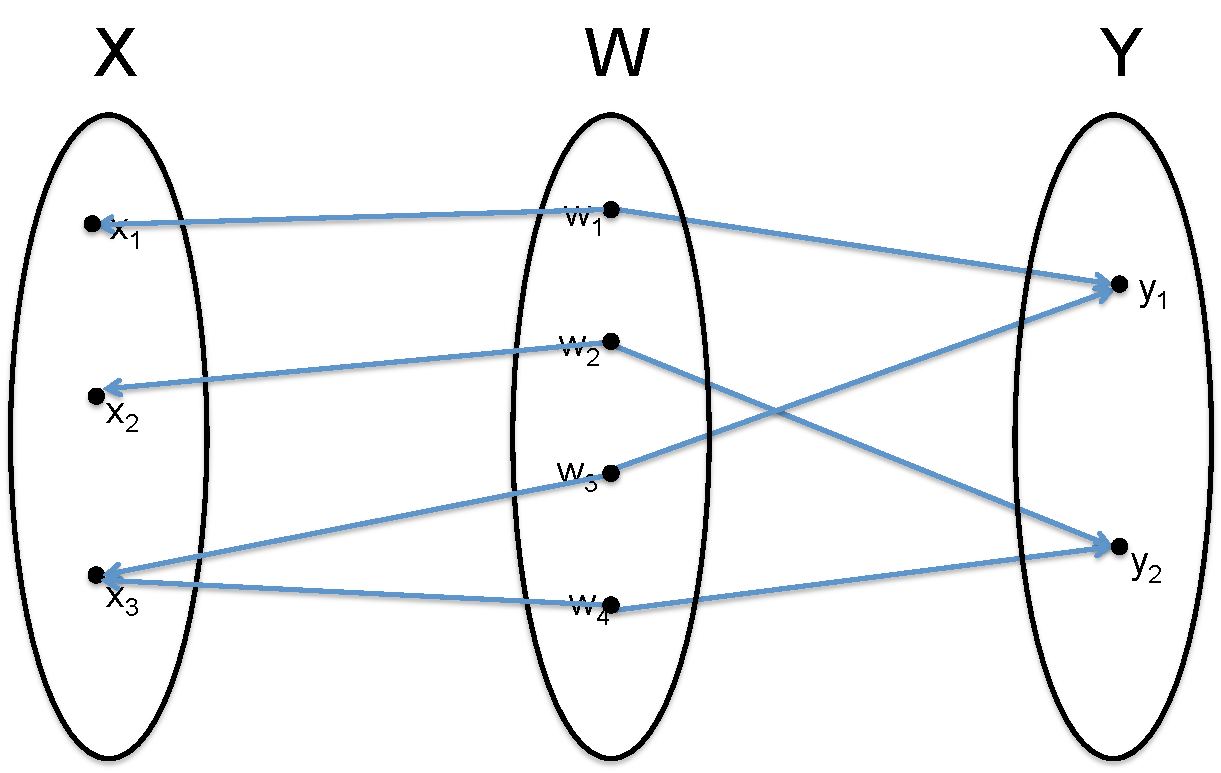
\includegraphics[height=2in]{setPushout}
\end{center}
The pushout of the diagram $X\Fromm{f}W\Too{g}Y$ is a set $P$. Write down the cardinality of $P\iso\ul{n}$ as a natural number $n\in\NN$.  
\end{exerciseENG}

\begin{exerciseRUS}
Пусть множества $W,X,Y$ и функции $f\taking W\to X$ и $g\taking W\to Y$ такие, как изображено ниже . 
\begin{center}
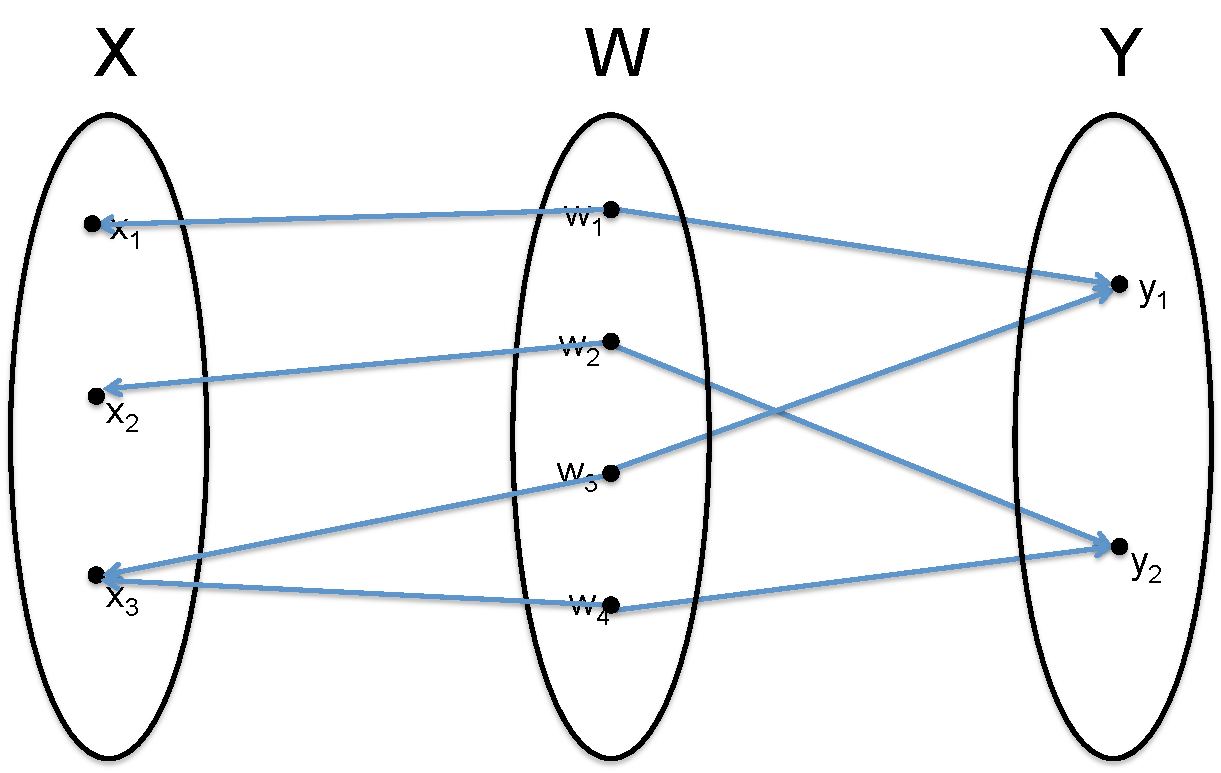
\includegraphics[height=2in]{setPushout}
\end{center}
Пушаут диаграммы $X\Fromm{f}W\Too{g}Y$ это множество $P$. Запишите мощность $P\iso\ul{n}$ в виде натурального числа $n\in\NN$.  
\end{exerciseRUS}

\begin{exerciseENG}
Suppose that $W=\emptyset$; what can you say about $X\sqcup_WZ$? 
\end{exerciseENG}

\begin{exerciseRUS}
Предположим, что $W=\varnothing$; что вы можете сказать о $X\sqcup_WZ$? 
\end{exerciseRUS}

\begin{exerciseENG}
Let $W:=\NN=\{0,1,2,\ldots\}$ denote the set of natural numbers, let $X=\ZZ$ denote the set of integers, and let $Y=\singleton$ denote a one-element set. Define $f\taking W\to X$ by $f(w)= -(w+1)$, and define $g\taking W\to Y$ to be the unique map. Describe the set $X\sqcup_WY$.
\end{exerciseENG}

\begin{exerciseRUS}
Пусть $W:=\NN=\{0,1,2,\ldots\}$ обозначает множество всех натуральных чисел, $X=\ZZ$ — можество всех целых чисел, и $Y=\singleton$ — одноэлементное множество. Определим $f\taking W\to X$ как $f(w)= -(w+1)$, и $g\taking W\to Y$ как единственное отображение такого вида. Опишите множество $X\sqcup_WY$.
\end{exerciseRUS}

\begin{exerciseENG}
Let $i\taking R\ss X\times X$ be an equivalence relation (see Example \ref{ex:subset as function} for notation). Composing with the projections $\pi_1,\pi_2\taking X\times X\to X$, we have two maps $\pi_1\circ i,\taking R\to X$ and $\pi_2\circ i\taking R\to X$. 
\sexc What is the pushout $$X\From{\pi_1\circ i}R\To{\pi_2\circ i}X?$$ 
\next If $i\taking R\ss X\times X$ is not assumed to be an equivalence relation, we can still define the pushout above. Is there a relationship between the pushout $X\From{\pi_1\circ i}R\To{\pi_2\circ i}X$ and the equivalence relation generated by $R\ss X\times X$?
\endsexc
\end{exerciseENG}

\begin{exerciseRUS}
Пусть $i\taking R\ss X\times X$ — это отношение эквивалентности (про обозначения см. Пример \ref{ex:subset as function}). Беря композицию с проекциями $\pi_1,\pi_2\taking X\times X\to X$, получим два отображения $\pi_1\circ i\taking R\to X$ и $\pi_2\circ i\taking R\to X$. 
\sexc Каким будет пушаут $$X\From{\pi_1\circ i}R\To{\pi_2\circ i}X?$$ 
\next Даже если $i\taking R\ss X\times X$ не обязательно отношение эквивалентности, мы все равно можем определить такой пушаут, как выше. Имеется ли связь между пушаутом $X\From{\pi_1\circ i}R\To{\pi_2\circ i}X$ и отношением эквивалентности, порожденным $R\ss X\times X$?
\endsexc
\end{exerciseRUS}

\begin{lemmaENG}[Universal property for pushout]\label{lemma:up for po}
Suppose given the diagram of sets and functions as below.
\begin{align*}
\xymatrix{W\ar[r]^u\ar[d]_t&Y\\
X}
\end{align*}
For any set $A$ and commutative solid arrow diagram as below (i.e. functions $f\taking X\to A$ and $g\taking Y\to A$ such that $f\circ t=g\circ u$), 
\begin{align}\label{dia:universal property of po}
\xymatrix{
&W\ar[dr]^u\ar[dl]_t\\
X\ar@/_1pc/[dddr]_{i_1}\ar[rd]_f&&Y\ar@/^1pc/[dddl]^{i_2}\ar[dl]^g\\
&A\\\\
&X\sqcup_WY\ar@{-->}[uu]^{\exists!}
}
\end{align}
there exists a unique arrow $\po{f}{g}{W}\taking X\sqcup_WY\to A$ making everything commute, $$f=\po{f}{g}{W}\circ i_1\hsp\text{and}\hsp g=\po{f}{g}{W}\circ i_2.$$
\end{lemmaENG}

\begin{lemmaRUS}[Универсальное свойство выталкивающего квадрата]\label{lemma:up for po}
Предположим, дана такая диаграмма множеств и функций, как ниже.
\begin{align*}
\xymatrix{W\ar[r]^u\ar[d]_t&Y\\
X}
\end{align*}
Для любого множества $A$ и коммутативной диаграммы (из сплошных стрелок) ниже (то есть функций $f\taking X\to A$ и $g\taking Y\to A$ таких, что $f\circ t=g\circ u$), 
\begin{align}\label{dia:universal property of po}
\xymatrix{
&W\ar[dr]^u\ar[dl]_t\\
X\ar@/_1pc/[dddr]_{i_1}\ar[rd]_f&&Y\ar@/^1pc/[dddl]^{i_2}\ar[dl]^g\\
&A\\\\
&X\sqcup_WY\ar@{-->}[uu]^{\exists!}
}
\end{align}
существует единственная стрелка $\po{f}{g}{W}\taking X\sqcup_WY\to A$, делающая коммутативной всю диаграмму, $$f=\po{f}{g}{W}\circ i_1\hsp\text{and}\hsp g=\po{f}{g}{W}\circ i_2.$$
\end{lemmaRUS}

%%%% Subsection %%%%

\subsection{Other finite colimits / Другие конечные копределы}

\begin{definitionENG}\label{def:coequalizer}[Coequalizer]\index{coequalizer}
Suppose given two parallel arrows 
\begin{align}\label{dia:coequalizer}
\xymatrix{X\ar@<.5ex>[r]^f\ar@<-.5ex>[r]_g&Y.}\hspace{1in}\xymatrix{X\ar@<.5ex>[r]^f\ar@<-.5ex>[r]_g&Y\ar[r]^-q&Coeq(f,g)}
\end{align}
The {\em coequalizer of $f$ and $g$} is the commutative diagram as to the right in (\ref{dia:coequalizer}), where we define $$Coeq(f,g):=Y\;/\;f(x)\sim g(x)$$ i.e. the coequalizer of $f$ and $g$ is the quotient of $Y$ by the equivalence relation generated by $\{(f(x),g(x))\|x\in X\}\ss Y\times Y$
\end{definitionENG}

\begin{definitionRUS}\label{def:coequalizer}[Коуравнитель]\index{coequalizer}
 
\end{definitionRUS}

\begin{exerciseENG}
Let $X=\RR$ be the set of real numbers. What is the coequalizer of the two maps $X\to X$ given by $x\mapsto x$ and $x\mapsto (x+1)$ respectively?
\end{exerciseENG}

\begin{exerciseRUS}
 
\end{exerciseRUS}

\begin{exerciseENG}
Find a universal property enjoyed by the coequalizer of two arrows.
\end{exerciseENG}

\begin{exerciseRUS}
 
\end{exerciseRUS}

\begin{exerciseENG}[Initial object]\label{exc:initial set}
An initial set is a set $S$ such that for every set $A$, there exists a unique function $S\to A$. 
\sexc Find an initial set. 
\next Do you think that the notion {\em initial set} belongs in this section (Section \ref{sec:finite colimits})? How so? If coproducts, pushouts, and coequalizers are all colimits, what do colimits have in common?
\endsexc
\end{exerciseENG}

\begin{exerciseRUS}[Инициальный объект]\label{exc:initial set}
 
\end{exerciseRUS}

%%%%%% Section %%%%%%

\section{Other notions in $\Set$ / Другие понятия в $\Set$}

In this section we discuss some left-over notions in the category of Sets.

В данном разделе мы обсудим некоторые из оставшихся понятий в категории множеств. 

%%%% Subsection %%%%

\subsection{Retractions / Ретракции}

\begin{definitionENG}
Suppose we have a function $f\taking X\to Y$ and a function $g\taking Y\to X$ such that $g\circ f=\id_X$. In this case we call $f$ a {\em retract section} and we call $g$ a {\em retract projection}. \index{retraction}
\end{definitionENG}

\begin{definitionRUS}
 
\end{definitionRUS}

\begin{exerciseENG}
Create an olog that includes sets $X$ and $Y$, and functions $f\taking X\to Y$ and $g\taking Y\to X$ such that $g\circ f=\id_X$ but such that $f\circ g\neq\id_Y$; that is, such that $f$ is a retract section but not an isomorphism.
\end{exerciseENG}

\begin{exerciseRUS}
 
\end{exerciseRUS}

%%%% Subsection %%%%

\subsection{Currying / Каррирование}\label{sec:currying}\index{currying}\index{materials!force extension curves}

Currying is the idea that when a function takes many inputs, we can input them one at a time or all at once. For example, consider the function that takes a material $M$ and an extension $E$ and returns the force transmitted through the material when it is pulled to that extension. This is a function $e\taking \fakebox{a material}\times\fakebox{an extension}\to\fakebox{a force}$. This function takes two inputs at once, but it is convenient to “curry” the second input. Recall that $\Hom_\Set(\fakebox{an extension},\fakebox{a force})$ is the set of theoretical force-extension curves. Currying transforms $e$ into a function $$e'\taking\fakebox{a material}\to\Hom_\Set(\fakebox{an extension},\fakebox{a force}).$$ This is a more convenient way to package the same information. 

 

In fact, it may be convenient to repackage this information another way. For any extension, we may want the function that takes a material and returns how much force it can transmit at that extension. This is a function $$e''\taking\fakebox{an extension}\to\Hom_\Set(\fakebox{a material},\fakebox{a force}).$$ 

 

\begin{notationENG}\index{exponentials ! in $\Set$}
Let $A$ and $B$ be sets. We sometimes denote the set of functions from $A$ to $B$ by 
\begin{align}\label{dia:exponential sets}
B^A:=\Hom_\Set(A,B).
\end{align}
\end{notationENG}

\begin{notationRUS}\index{exponentials ! in $\Set$}
 
\end{notationRUS}

\begin{exerciseENG}
For a finite set $A$, let $|A|\in\NN$ denote the cardinality of (number of elements in) $A$. If $A$ and $B$ are both finite (including the possibility that one or both are empty), is it always true that $|B^A|=|B|^{|A|}$?
\end{exerciseENG}

\begin{exerciseRUS}
 
\end{exerciseRUS}

\begin{propositionENG}[Currying]\label{prop:curry}
Let $A$ denote a set. For any sets $X,Y$ there is a bijection 
\begin{align}\label{dia:curry bijection}
\phi\taking\Hom_\Set(X\times A,Y)\To{\iso}\Hom_\Set(X,Y^A).
\end{align}
\end{propositionENG}

\begin{propositionRUS}[Каррирование]\label{prop:curry}
 
\end{propositionRUS}

\begin{proofENG}
Suppose given $f\taking X\times A\to Y$. Define $\phi(f)\taking X\to Y^A$ as follows: for any $x\in X$ let $\phi(f)(x)\taking A\to Y$ be defined as follows: for any $a\in A$, let $\phi(f)(x)(a):=f(x,a)$. 

We now construct the inverse, $\psi\taking\Hom_\Set(X,Y^A)\to\Hom_\Set(X\times A,Y)$. Suppose given $g\taking X\to Y^A$. Define $\psi(g)\taking X\times A\to Y$ as follows: for any pair $(x,a)\in X\times A$ let $\psi(g)(x,a):=g(x)(a)$. 

Then for any $f\in\Hom_\Set(X\times A,Y)$ we have $\psi\circ\phi(f)(x,a)=\phi(f)(x)(a)=f(x,a)$, and for any $g\in\Hom_\Set(X,Y^A)$ we have $\phi\circ\psi(g)(x)(a)=\psi(g)(x,a)=g(x)(a)$, Thus we see that $\phi$ is an isomorphism as desired.
\end{proofENG}

\begin{proofRUS}
 
\end{proofRUS}

\begin{exerciseENG}
Let $X=\{1,2\}, A=\{a,b\}$, and $Y=\{x,y\}$. 
\sexc\label{part:three distinct} Write down three distinct elements of $L:=\Hom_\Set(X\times A,Y)$. 
\next Write down all the elements of $M:=\Hom_\Set(A,Y)$. 
\next For each of the three elements $\ell\in L$ you chose in part (\ref{part:three distinct}), write down the corresponding function $\phi(\ell)\taking X\to M$ guaranteed by Proposition \ref{prop:curry}.
\endsexc
\end{exerciseENG}

\begin{exerciseRUS}
 
\end{exerciseRUS}

\begin{exerciseENG}\label{exc:evaluation}\index{exponentials!evaluation of}
Let $A$ and $B$ be sets. We know that $\Hom_\Set(A,B)=B^A$, so we have a function $\id_{B^A}\taking\Hom_\Set(A,B)\to B^A$. Look at Proposition \ref{prop:curry}, making the substitutions $X=\Hom_\Set(A,B)$, $Y=B$, and  $A=A$. Consider the function $$\phi^\m1\taking\Hom_\Set(\Hom_\Set(A,B),B^A)\to\Hom_\Set(\Hom_\Set(A,B)\times A,B)$$ obtained as the inverse of (\ref{dia:curry bijection}). We have a canonical element $\id_{B^A}$ in the domain of $\phi^\m1$. We can apply the function $\phi^\m1$ and obtain an element $ev=\phi^\m1(\id_{B^A})\in\Hom_\Set(\Hom_\Set(A,B)\times A,B)$, which is itself a function, $$ev\taking\Hom_\Set(A,B)\times A\to B.$$ 
\sexc Describe the function $ev$ in terms of how it operates on elements in its domain. 
\next Why might one be tempted to denote this function by $ev$?
\endsexc
\end{exerciseENG}

\begin{exerciseRUS}\label{exc:evaluation}\index{exponentials!evaluation of}
 
\end{exerciseRUS}

If $n\in\NN$ is a natural number, recall from (\ref{dia:underline n}) that there is a nice set $\ul{n}=\{1,2,\ldots,n\}$. If $A$ is a set, we often make the abbreviation 
\begin{align}\label{dia:exponential abbrev}
A^n:=A^{\ul{n}}.
\end{align}

 

\begin{exerciseENG}\label{exc:two R2s}
In Example \ref{ex:R2} we said that $\RR^2$ is an abbreviation for $\RR\times\RR$, but in (\ref{dia:exponential abbrev}) we say that $\RR^2$ is an abbreviation for $\RR^{\ul{2}}$. Use Exercise \ref{exc:generator for set}, Proposition \ref{prop:curry}, Exercise \ref{exc:coprod}, and the fact that 1+1=2, to prove that these are isomorphic, $\RR^{\ul{2}}\iso\RR\times\RR$.

(The answer to Exercise \ref{exc:generator for set} was $A=\singleton$: i.e. $\Hom_\Set(\singleton,X)\iso X$ for all $X$.)
\end{exerciseENG}

\begin{exerciseRUS}\label{exc:two R2s}
 
\end{exerciseRUS}

%%%% Subsection %%%%

\subsection{Arithmetic of sets / Арифметика множеств}\label{sec:arithmetic of sets}\index{set!arithmetic of}

Proposition \ref{prop:arithmetic of sets} summarizes the properties of products, coproducts, and exponentials, and shows them all in a familiar light, namely that of arithmetic. In fact, one can think of the natural numbers as literally being the isomorphism classes of finite sets — that's what they are used for in counting. Consider the standard procedure for counting the elements of a set $S$, say cows in a field: one points to an element in $S$ and simultaneously says “1”, points to another element in $S$ and simultaneously says “2”, and so on until finished. This procedure amounts to nothing more than creating an isomorphism (one-to-one mapping) between $S$ and some set $\ul{n}$. 

 

Again, the natural numbers are the isomorphism classes of finite sets. Their behavior, i.e. the arithmetic of natural numbers, reflects the behavior of sets. For example the fact that multiplication distributes over addition is a fact about grids of dots as in Example \ref{ex:grid1}. The following proposition lays out such arithmetic properties of sets.

 

In this proposition, we denote the coproduct of two sets $A$ and $B$ by the notation $A+B$ rather than $A\sqcup B$. It is a reasonable notation in general, and one that is often used. 

 

\begin{propositionENG}\label{prop:arithmetic of sets}
The following isomorphisms exist for any sets $A,B,$ and $C$ (except for one caveat, see Exercise \ref{exc:0 to the 0}). 
 
\begin{itemize}
\item $A+\ul{0}\iso A$
\item $A + B\iso B + A$
\item $(A + B) + C \iso A + (B + C)$
\item $A\times\ul{0}\iso\ul{0}$
\item $A\times\ul{1}\iso A$
\item $A\times B\iso B\times A$
\item $(A\times B)\times C \iso A\times (B\times C)$
\item $A\times(B+C)\iso (A\times B)+(A\times C)$
\item $A^{\ul{0}}\iso \ul{1}$
\item $A^{\ul{1}}\iso A$
\item $\ul{0}^A\iso\ul{0}$
\item $\ul{1}^A\iso\ul{1}$
\item $A^{B+C}\iso A^B\times A^C$
\item $(A^B)^C\iso A^{B\times C}$
\end{itemize}
\end{propositionENG}

\begin{propositionRUS}\label{prop:arithmetic of sets}
 
\end{propositionRUS}

\begin{exerciseENG}\label{exc:0 to the 0}
Everything in Proposition \ref{prop:arithmetic of sets} is true except in one case, namely that of $$\ul{0}^{\ul{0}}.$$ In this case, we get conflicting answers, because for any set $A$, including $A=\emptyset=\ul{0}$, we have claimed both that $A^{\ul{0}}\iso\ul{1}$ and that $\ul{0}^A\iso\ul{0}.$ 

What is the correct answer for $\ul{0}^{\ul{0}}$, based on the definitions of $\ul{0}$ and $\ul{1}$, given in (\ref{dia:underline n}), and of $A^B$, given in (\ref{dia:exponential sets})?
\end{exerciseENG}

\begin{exerciseRUS}\label{exc:0 to the 0}
 
\end{exerciseRUS}

\begin{exerciseENG}
It is also true of natural numbers that if $a,b\in\NN$ and $ab=0$ then either $a=0$ or $b=0$. Is the analogous statement true of all sets?
\end{exerciseENG}

\begin{exerciseRUS}
 
\end{exerciseRUS}

Proposition \ref{prop:arithmetic of sets} is in some sense about isomorphisms. It says that understanding isomorphisms of sets reduces to understanding natural numbers. But note that there is much more going on in $\Set$ than isomorphisms; in particular there are functions that are not invertible. 

 

In grade school you probably never saw anything that looked like this:
$$5^3\times 3\too 5$$
And yet in Exercise \ref{exc:evaluation} we found a function $ev\taking B^A\times A\to B$ that exists for any sets $A,B$. This function $ev$ is not an isomorphism so it somehow does not show up as an equation of natural numbers. But it still has important meaning.%
\footnote{Roughly, the existence of $ev\taking\ul{5}^{\ul{3}}\times\ul{3}\too \ul{5}$ says that given a dot in a $5\times 5\times 5$ grid of dots, and given one of the three axes, you can tell me the coordinate of that dot along that axis.} In terms of mere number, it looks like we are being told of an important function $\ul{575}\to\ul{5}$, which is bizarre. The issue here is precisely the one you confronted in Exercise \ref{exc:functions are not iso invariant}.

 

\begin{exerciseENG}
Explain why there is a canonical function $\ul{5}^{\ul{3}}\times\ul{3}\too \ul{5}$ but not a canonical function $\ul{575}\to\ul{5}$.
\end{exerciseENG}

\begin{exerciseRUS}
 
\end{exerciseRUS}

\begin{sloganENG}
It is true that a set is isomorphic to any other set with the same number of elements, but don't be fooled into thinking that the study of sets reduces to the study of numbers. Functions that are not isomorphisms cannot be captured within the framework of numbers. 
\end{sloganENG}

\begin{sloganRUS}
 
\end{sloganRUS}

%%%% Subsection %%%%

\subsection{Subobjects and characteristic functions / Подобъекты и характеристические функции}

\begin{definitionENG}\label{def:power set}
For any set $B$, define the {\em power set of $B$}\index{power set}, denoted $\PP(B)$,\index{a symbol!$\PP$} to be the set of subsets of $B$.
\end{definitionENG}

\begin{definitionRUS}\label{def:power set}
 
\end{definitionRUS}

\begin{exerciseENG}\label{exc:size of power sets}~
\sexc How many elements does $\PP(\emptyset)$ have? 
\next How many elements does $\PP(\singleton)$ have? 
\next How many elements does $\PP(\{1,2,3,4,5,6\})$ have? 
\next Any idea why they may have named it “power set”?
\endsexc
\end{exerciseENG}

\begin{exerciseRUS}\label{exc:size of power sets}~
 
\end{exerciseRUS}

%% Subsubsection %%

\subsubsection{Simplicial complexes / Симплициальные комплексы}\label{sec:simplicial complex}

\begin{definitionENG}\label{def:simplicial complex}\index{simplicial complex}
Let $V$ be a set and let $\PP(V)$ be its powerset. A subset $X\ss\PP(V)$ is called {\em downward-closed} if, for every $u\in X$ and every $u'\ss u$, we have $u'\in X$. We say that $X$ {\em contains all atoms} if for every $v\in V$ the singleton set $\{v\}$ is an element of $X$. 

A {\em simplicial complex} is a pair $(V,X)$ where $V$ is a set and $X\ss\PP(V)$ is a downward-closed subset that contains all atoms. The elements of $X$ are called {\em simplices} (singular: {\em simplex}).\index{simplex} Any subset $u\ss V$ has a cardinality $|u|$, so we have a function $X\to\NN$ sending each simplex to its cardinality. The set of simplices with cardinality $n+1$ is denoted $X_n$ and each element $x\in X_n$ is called an {\em $n$-simplex}.%
\footnote{It is annoying at first that the set of subsets with cardinality 1 is denoted $X_0$, etc. But this is standard convention because as we will see, $X_n$ will be $n$-dimensional.}
Since $X$ contains all atoms (subsets of cardinality 1), we have $X_0\iso V$, and we may also call the 0-simplices {\em vertices}. We sometimes call the 1-simplices {\em edges}.%
\footnote{The reason we wrote $X_0\iso V$ rather than $X_0=V$ is that $X_0$ is the set of 1-element subsets of $V$. So if $V=\{a,b,c\}$ then $X_0=\{\{a\},\{b\},\{c\}\}$. This is really just pedantry.}

Since $X_0\iso V$, we may denote a simplicial complex $(V,X)$ simply by $X$.
\end{definitionENG}

\begin{definitionRUS}\label{def:simplicial complex}\index{simplicial complex}
 
\end{definitionRUS}

\begin{exampleENG}
Let $n\in\NN$ be a natural number and let $V=\ul{n+1}$. Define {\em the $n$-simplex}, denoted $\Delta^n$, to be the simplicial complex $\PP(V)\ss\PP(V)$, i.e. the whole power set, which indeed is downward-closed and contains all atoms. 
\end{exampleENG}

\begin{exampleRUS}
 
\end{exampleRUS}

We can draw a simplicial complex $X$ by first putting all the vertices on the page as dots. Then for every $x\in X_1$, we see that $x=\{v,v'\}$ consists of 2 vertices, so we draw an edge connecting $v$ and $v'$. For every $y\in X_2$ we see that $y=\{w,w',w''\}$ consists of 3 vertices, so we draw a (filled-in) triangle connecting them. All three edges will be drawn too because $X$ is assumed to be downward closed.

 

Thus, the 0-simplex $\Delta^0$, the 1-simplex $\Delta^1$, the 2-simplex $\Delta^2$, and the 3-simplex $\Delta^3$ are drawn here:
\begin{center}
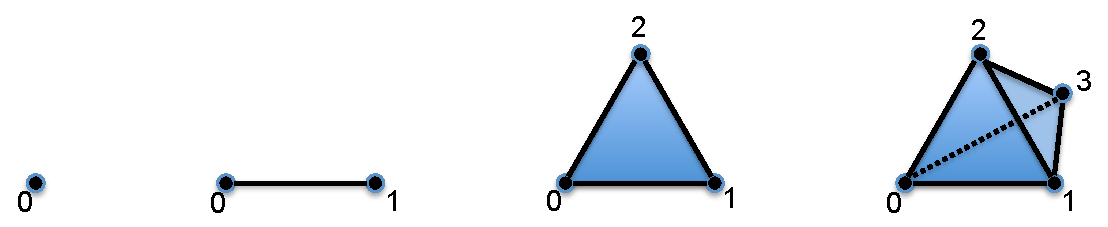
\includegraphics[height=1.1in]{simplices}
\end{center} 

 

The $n$-simplices for various $n$'s are in no way all of the simplicial complexes. In general a simplicial complex is a union or “gluing together” of simplices in a prescribed manner. For example, consider the simplicial complex $X$ with vertices $X_0=\{1,2,3,4\},$ edges $X_1=\{\{1,2\},\{2,3\},\{2,4\}\},$ and no higher simplices $X_2=X_3=\cdots=\emptyset$. We might draw $X$ as follows:
$$\xymatrix{\LMO{1}\ar@{-}[r]&\LMO{2}\ar@{-}[r]\ar@{-}[d]&\LMO{3}\\&\LMO{4}}$$

 

\begin{exerciseENG}
Let $X$ be the following simplicial complex, so that $X_0=\{A,B,\ldots,M\}$. 
\begin{center}
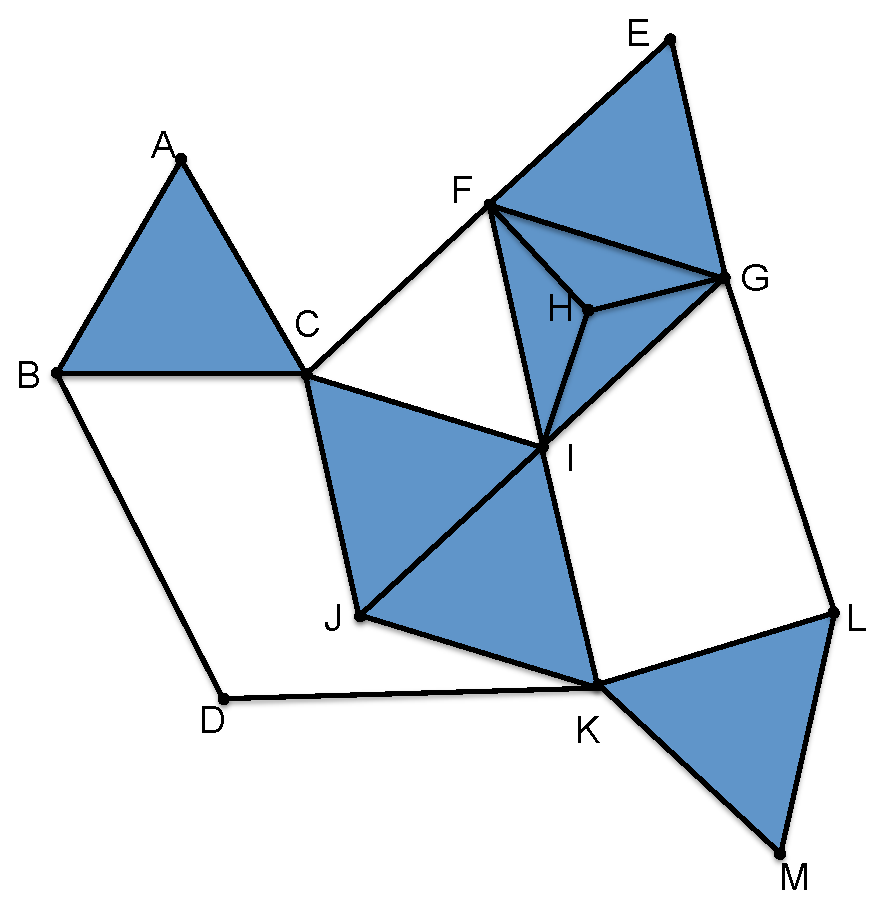
\includegraphics[height=3in]{OlogNetwork5}
\end{center} 
In this case $X_1$ consists of elements like $\{A,B\}$ and $\{D,K\}$ but not $\{D,J\}$. 

Write out $X_2$ and $X_3$ (hint: the drawing of $X$ indicates that $X_3$ should have one element).
\end{exerciseENG}

\begin{exerciseRUS}
 
\end{exerciseRUS}

\begin{exerciseENG}
The 2-simplex $\Delta^2$ is drawn as a filled-in triangle with vertices $V=\{1,2,3\}$. There is a simplicial complex $X=\partial\Delta^2$ that would be drawn as an empty triangle with the same set of vertices. 
\sexc Draw $\Delta^2$ and $X$ side by side and make clear the difference.
\next Write down the data for $X$ as a simplicial complex. In other words what are the sets $X_0, X_1, X_2, X_3,\ldots$?
\endsexc
\end{exerciseENG}

\begin{exerciseRUS}
 
\end{exerciseRUS}

%% Subsubsection %%

\subsubsection{Subobject classifier / Классификатор подобъектов}

\begin{definitionENG}\label{def:subobject classifier}\index{subobject classifier!in $\Set$}
Define the {\em subobject classifier} for $\Set$, denoted $\Omega$\index{a symbol!$\Omega$}, to be the set $\Omega:=\{True,False\}$, together with the function $\singleton\to\Omega$ sending the unique element to $True$.
\end{definitionENG}

\begin{definitionRUS}\label{def:subobject classifier}\index{subobject classifier!in $\Set$}
 
\end{definitionRUS}

\begin{propositionENG}\label{prop:characteristic function}
Let $B$ be a set. There is an isomorphism $$\phi\taking\Hom_\Set(B,\Omega)\To{\iso}\PP(B).$$
\end{propositionENG}

\begin{propositionRUS}\label{prop:characteristic function}
 
\end{propositionRUS}

\begin{proofENG}
Given a function $f\taking B\to\Omega$, let $\phi(f)=\{b\in B\|f(b)=True\}\ss B$. We now construct a function $\psi\taking\PP(B)\to\Hom_\Set(B,\Omega)$ to serve as the inverse of $\phi$. Given a subset $B'\ss B$, define $\psi(B')\taking B\to\Omega$ as follows: 
$$\psi(i)(b)=\begin{cases}
True&\tn{ if } b\in B',\\
False&\tn{ if } b\not\in B'.
\end{cases}
$$
One checks easily that $\phi$ and $\psi$ are mutually inverse.
\end{proofENG}

\begin{proofRUS}
 
\end{proofRUS}

\begin{definitionENG}[Characteristic function]\index{characteristic function}\index{subset!characteristic function of}

Given a subset $B'\ss B$, we call the corresponding function $B\to\Omega$ the {\em characteristic function of $B'$ in $B$.}
\end{definitionENG}

\begin{definitionRUS}[Characteristic function]\index{characteristic function}\index{subset!characteristic function of}
 
\end{definitionRUS}

Let $B$ be any set and let $\PP(B)$ be its power set. By Proposition \ref{prop:characteristic function} there is a bijection between $\PP(B)$ and $\Omega^B$. Since $\Omega$ has cardinality 2, the cardinality of $\PP(B)$ is $2^{|B|}$, which explains the correct answer to Exercise \ref{exc:size of power sets}.

 

\begin{exerciseENG}
Let $f\taking A\to\Omega$ denote the characteristic function of some $A'\ss A$, and define $A''\ss A$ to be its complement, $A'':=A-A'$ (i.e. $a\in A''$ if and only if $a\not\in A'$). 
\sexc What is the characteristic function of $A''\ss A$? 
\next Can you phrase it in terms of some function $\Omega\to\Omega$?
\endsexc
\end{exerciseENG}

\begin{exerciseRUS}
 
\end{exerciseRUS}

%%%% Subsection %%%%

\subsection{Surjections, injections / Сюръекции, инъекции}

The classical definition of injections and surjections involves elements, which we give now. But a more robust notion involves all maps and will be given in Proposition \ref{prop:inj and surj}.

 

\begin{definitionENG}\label{def:inj,surj,bij}\index{function!injection}\index{function!surjection}\index{function!bijection}
Let $f\taking X\to Y$ be a function. We say that $f$ is {\em surjective} if, for all $y\in Y$ there exists some $x\in X$ such that $f(x)=y$. We say that $f$ is {\em injective} if, for all $x\in X$ and all $x'\in X$ with $f(x)=f(x')$ we have $x=x'$.

A function that is both injective and surjective is called {\em bijective}.
\end{definitionENG}

\begin{definitionRUS}\label{def:inj,surj,bij}\index{function!injection}\index{function!surjection}\index{function!bijection}
 
\end{definitionRUS}

\begin{remarkENG}
It turns out that a function that is bijective is always an isomorphism and that all isomorphisms are bijective. We will not show that here, but it is not too hard; see for example \cite[Theorem 5.4]{Big}.
\end{remarkENG}

\begin{remarkRUS}
 
\end{remarkRUS}

\begin{definitionENG}[Monomorphisms, epimorphisms]\label{def:mono, epi in set}\index{epimorphism!in $\Set$}\index{monomorphism!in $\Set$}
Let $f\taking X\to Y$ be a function. 

We say that $f$ is a {\em monomorphism} if for all sets $A$ and pairs of functions $g,g'\taking A\to X$,
$$
\xymatrix{A\ar@/^1pc/[r]^g\ar@/_1pc/[r]_{g'}&X\ar[r]^f&Y}
$$
if $f\circ g=f\circ g'$ then $g=g'$.

We say that $f$ is an {\em epimorphism} if for all sets $B$ and pairs of functions $h,h'\taking Y\to B$, 
$$
\xymatrix{X\ar[r]^f&Y\ar@/^1pc/[r]^h\ar@/_1pc/[r]_{h'}&B}
$$
if $h\circ f=h'\circ f$ then $h=h'$.
\end{definitionENG}

\begin{definitionRUS}[Мономорфизмы, эпиморфизмы]\label{def:mono, epi in set}\index{epimorphism!in $\Set$}\index{monomorphism!in $\Set$}
 
\end{definitionRUS}

\begin{propositionENG}\label{prop:inj and surj}
Let $f\taking X\to Y$ be a function. Then $f$ is injective if and only if it is a monomorphism; $f$ is surjective if and only if it is an epimorphism.
\end{propositionENG}

\begin{propositionRUS}\label{prop:inj and surj}
 
\end{propositionRUS}

\begin{proofENG}
If $f$ is a monomorphism it is clearly injective by putting $A=\singleton$. Suppose that $f$ is injective and let $g,g'\taking A\to X$ be functions such that $f\circ g=f\circ g'$, but suppose for contradiction that $g\neq g'$. Then there is some element $a\in A$ such $g(a)\neq g'(a)\in X$. But by injectivity $f(g(a))\neq f(g'(a))$, contradicting $f\circ g=f\circ g'$.

Suppose that $f\taking X\to Y$ is an epimorphism and choose some $y_0\in Y$ (noting that if $Y$ is empty then the claim is vacuously true). Let $h\taking Y\to\Omega$ denote the characteristic function of the subset $\{y_0\}\ss Y$ and let $h'\taking Y\to\Omega$ denote the characteristic function of $\emptyset\ss Y$; note that $h(y)=h'(y)$ for all $y\neq y_0$. Then since $f$ is an epimorphism and $h\neq h'$, we must have $h\circ f\neq h'\circ f$, so there exists $x\in X$ with $h(f(x))\neq h'(f(x))$, which implies that $f(x)=y_0$. This proves that $f$ is surjective.

Finally, suppose that $f$ is surjective, and let $h,h'\taking Y\to B$ be functions with $h\circ f=h'\circ f$. For any $y\in Y$, there exists some $x\in X$ with $f(x)=y$, so $h(y)=h(f(x))=h'(f(x))=h'(y)$. This proves that $f$ is an epimorphism.
\end{proofENG}

\begin{proofRUS}
 
\end{proofRUS}

\begin{propositionENG}\label{prop:pb preserve mono}
Let $f\taking X\to Y$ be a monomorphism. Then for any function $g\taking A\to Y$, the top map $f'\taking X\times_YA\to A$ in the diagram
$$
\xymatrix{X\times_YA\ar[r]^-{f'}\ar[d]_{g'}\ullimit&A\ar[d]^g\\X\ar[r]_f&Y}
$$
is a monomorphism.
\end{propositionENG}

\begin{propositionRUS}\label{prop:pb preserve mono}
 
\end{propositionRUS}

\begin{proofENG}
To show that $f'$ is a monomorphism, we take an arbitrary set $B$ and two maps $m,n\taking B\to X\times_YA$ such that $f'\circ m=f'\circ n$, denote that function by $p:=f'\circ m\taking B\to A$. Now let $q=g'\circ m$ and $r=g'\circ n$. The diagram looks like this:
$$
\xymatrix{B\ar@<.5ex>[rr]^(.4)m\ar@<-.5ex>[rr]_(.4)n\ar@/^2pc/[rrr]^p\ar@<.5ex>[drr]^(.6)q\ar@<-.5ex>[drr]_(.6)r&&X\times_YA\ar[r]^{f'}\ar[d]_{g'}\ullimit&A\ar[d]^g\\&&X\ar[r]_f&Y}
$$
We have that 
\begin{align*}f\circ q=f\circ g'\circ m=g\circ f'\circ m=g\circ f'\circ n=f\circ g'\circ n=f\circ r\end{align*} 
But we assumed that $f$ is a monomorphism so this implies that $q=r$. By the universal property of pullbacks, Lemma \ref{lemma:up for fp}, we have $m=n$.
\end{proofENG}

\begin{proofRUS}
 
\end{proofRUS}

\begin{exerciseENG}
Show, in analogy to Proposition \ref{prop:pb preserve mono}, that pushouts preserve epimorphisms.
\end{exerciseENG}

\begin{exerciseRUS}
 
\end{exerciseRUS}

\begin{exampleENG}\label{exc:olog pullbacks}
Suppose an olog has a fiber product square
$$\xymatrix{X\times_ZY\ar[r]^-{g'}\ar[d]_{f'}&Y\ar[d]^f\\X\ar[r]_g&Z}$$ such that $f$ is intended to be an injection and $g$ is any map.%
\footnote{Of course, this diagram is symmetrical, so the same ideas hold if $g$ is an injection and $f$ is any map.} 
In this case, there are nice labeling systems for $f', g'$, and $X\times_ZY$. Namely:
\begin{itemize}
\item “is” is an appropriate label for $f'$, 
\item the label for $g$ is an appropriate label for $g'$,
\item (the label for $X$, then “which”, then the label for $g$, then the label for $Y$) is an appropriate label for $X\times_ZY$.
\end{itemize}

To give an explicit example, 
$$\xymatrix{
\obox{X\times_ZY}{.9in}{a rib which is made by a cow}\LA{rr}{is made by}\LAL{d}{is}&&\obox{Y}{.4in}{a cow}\LA{d}{is}\\
\obox{X}{.3in}{a rib}\LAL{rr}{is made by}&&\obox{Z}{.6in}{an animal}
}
$$
\end{exampleENG}

\begin{exampleRUS}\label{exc:olog pullbacks}
 
\end{exampleRUS}

\begin{corollaryENG}\label{cor:monos are pullbacks of true}
Let $i\taking A\to X$ be a monomorphism. Then there is a fiber product square of the form 
\begin{align}\label{dia:monos are pbs of true}
\xymatrix{A\ar[r]^{f'}\ar[d]_i\ullimit&\singleton\ar[d]^{True}\\X\ar[r]_f&\Omega.}
\end{align}
\end{corollaryENG}

\begin{corollaryRUS}\label{cor:monos are pullbacks of true}
 
\end{corollaryRUS}

\begin{proofENG}
Let $X'\ss X$ denote the image of $i$ and let $f\taking X\to\Omega$ denote the characteristic function of $X'\ss X$. Then it is easy to check that Diagram \ref{dia:monos are pbs of true} is a pullback.
\end{proofENG}

\begin{proofRUS}
 
\end{proofRUS}

\begin{exerciseENG}
Consider the subobject classifier $\Omega$, the singleton $\singleton$ and the map $\singleton\To{True}\Omega$ from Definition \ref{def:subobject classifier}. Look at diagram \ref{dia:monos are pbs of true} and in the spirit of Exercise \ref{exc:olog pullbacks}, come up with a label for $\Omega$, a label for $\singleton$, and a label for $True$. Given a label for $X$ and a label for $f$, come up with a label for $A$, a label for $i$ and a label for $f'$, such that the English smoothly fits the mathematics.
\end{exerciseENG}

\begin{exerciseRUS}
 
\end{exerciseRUS}

%%%% Subsection %%%%

\subsection{Multisets, relative sets, and set-indexed sets / Мультимножества, относительные множества, индексированные множества}

In this section we prepare ourselves for considering categories other than $\Set$, by looking at some categories related to $\Set$. 

 

%% Subsubsection %%

\subsubsection{Multisets / Мультимножества}\index{multiset}

Consider the set $X$ of words in a given document. If $WC(X)$ is the wordcount of the document, we will not generally have $WC(X)=|X|$. The reason is that a set cannot contain the same element more than once, so words like “the” might be undercounted in $|X|$. A {\em multiset} is a set in which elements can be assigned a multiplicity, i.e. a number of times they are to be counted. 

 

But if $X$ and $Y$ are multisets, what is the appropriate type of mapping from $X$ to $Y$? Since every set is a multiset (in which each element has multiplicity 1), let's restrict ourselves to notions of mapping that agree with the usual one on sets. That is, if multisets $X$ and $Y$ happen to be sets then our mappings $X\to Y$ should just be functions.

 

\begin{exerciseENG}\label{exc:multiset 1}~
\sexc Come up with some notion of mapping for multisets that generalizes functions when the notion is restricted to sets. 
\next Suppose that $X=(1,1,2,3)$ and $Y=(a,b,b,b)$, i.e. $X=\{1,2,3\}$ with $1$ having multiplicity 2, and $Y=\{a,b\}$ with $b$ having multiplicity 3. What are all the maps $X\to Y$ in your notion?
\endsexc
\end{exerciseENG}

\begin{exerciseRUS}\label{exc:multiset 1}~
 
\end{exerciseRUS}

In Chapter \ref{chap:categories} we will be getting to the definition of category, and you can test whether your notion of mapping in fact defines a category. Here is my definition of mapping for multisets.

 

\begin{definitionENG}\label{def:multiset}
A {\em multiset} is a sequence $X:=(E,B,\pi)$ where $E$ and $B$ are sets and $\pi\taking E\to B$ is a surjective function. We refer to $E$ as the set of {\em element instances of $X$}, we refer to $B$ as the set of {\em element names of $X$}, and we refer to $\pi$ as the {\em naming function for $X$}. Given an element name $x\in B$, let $\pi^\m1(x)\ss E$ be the preimage; the number of elements in $\pi^\m1(x)$ is called the {\em multiplicity of $x$}.

Suppose that $X=(E,B,\pi)$ and $X'=(E',B',\pi')$ are multisets. A {\em mapping from $X$ to $Y$}, denoted $f\taking X\to Y$, consists of a pair $(f_1,f_0)$ such that $f_1\taking E\to E'$ and $f_0\taking B\to B'$ are functions and such that the following diagram commutes:
\begin{align}\label{dia:multiset map}
\xymatrix{E\ar[r]^{f_1}\ar[d]_{\pi}&E'\ar[d]^{\pi'}\\B\ar[r]_{f_0}&B'.}
\end{align}
\end{definitionENG}

\begin{definitionRUS}\label{def:multiset}
 
\end{definitionRUS}

\begin{exerciseENG}
Suppose that a pseudo-multiset is defined to be almost the same as a multiset, except that $\pi$ is not required to be surjective. 
\sexc Write down a pseudo-multiset that is not a multi-set. 
\next Describe the difference between the two notions in terms of multiplicities. 
\next Complexity of names aside, which do you think is a more useful notion: multiset or pseudo-multisets? 
\endsexc
\end{exerciseENG}

\begin{exerciseRUS}
 
\end{exerciseRUS}

\begin{exerciseENG}
Consider the multisets described in Exercise \ref{exc:multiset 1}. 
\sexc Write each of them in the form $(E,B,\pi)$, as in Definition \ref{def:multiset}. 
\next In terms of the same definition, what are the mappings $X\to Y$? 
\next If we remove the restriction that diagram \ref{dia:multiset map} must commute, how many mappings $X\to Y$ are there?
\endsexc
\end{exerciseENG}

\begin{exerciseRUS}
 
\end{exerciseRUS}

%\begin{exampleENG}[Using multisets to approach probability]
%
%Let $S=\{a,b,c,d\}$, and call each element of $S$ a {\em suit}. Let $R=\{1,2,\ldots,13\}$, and call each element of $R$ a {\em rank}. Let $C=S\times R$, and call each element of $C$ a {\em card}. For each $n\in\NN$, let $$A_n=\{f\taking \{1,2,\ldots,n\}\to C\|f \tn{ is injective}\}$$ and call each element of $A_n$ an {\em $n$-card arrangement}. So $A_{52}$ has $52!:=52*51*\cdots*1$ elements and $A_1$ has 52 elements.
%
%The {\em 4-handed poker deal} is the function $A_{52}\to A_5\times A_5\times A_5\times A_5$ given as follows. For each $i\in\{1,2,3,4\}$, let $p_i\taking\{1,2,3,4,5\}\to\{1,2,\ldots,52\}$ be the (injective) function given by the following matrix
%\begin{align}
%\begin{array}{l || l | l | l | l | l}
%i&p_i(1)&p_i(2)&p_i(3)&p_i(4)&p_i(5)\\\hline
%p_1&1&5&9&13&17\\
%p_2&2&6&10&14&18\\
%p_3&3&7&11&15&19\\
%p_4&4&8&12&16&20
%\end{array}
%\end{align}
%Then if $f\taking\{1,2,\ldots,52\}\to C$ is a 52-card arrangement, then $f\circ p_i\taking\{1,2,3,4,5\}\to C$ is a 5-card arrangement, and putting them together we get our 4-handed poker deal.
%
%We could similarly define a $k$-handed poker deal for any $1\leq k\leq 10$. We focus here on $1$-handed poker deals. For any $n\leq 52$, let $\sim_n$ denote the equivalence relation on $A_n$ for which two arrangements are equivalent if one is a permutation (reordering) of the other. Let $H_n=A_n/\sim_n$ be the quotient; we call its elements {\em $n$-card hands}. 
%
%In “5-card poker”, the 5-card hands are classified by patterns of suits and ranks in the cards. More precisely, given a 5-card arrangement $f\taking \{1,2,3,4,5\}\to C$, we consider the compositions with $\pi_1\taking C\to S$ and $\pi_2\taking C\to R$, which we denote $f_S:=\pi_1\circ f$ and $f_R:=\pi_2\circ f$. We are concerned only with the cardinalities of the fibers of $f_S$ and $f_R$. For example if some suit $s\in S$ has $|f_S^\m1(s)|=5$ we say that $f$ (or its equivalence class in $H_5$) is a {\em flush}. If for ranks $r_1,r_2$ we have $|f_R^\m1(r_1)|=2$ and $|f_R^\m1(r_2)|=3$, we call it a {\em full house}. 
%
%\end{exampleENG}

%% Subsubsection %%

\subsubsection{Relative sets / Относительные множества}\label{sec:relative sets}\index{relative set}

Let's continue with our ideas from multisets, but now suppose that we have a fixed set $B$ of names that we want to keep once and for all. Whenever someone discusses a set, each element must have a name in $B$. And whenever someone discusses a mapping, it must preserve the names. For example, if $B$ is the set of English words, then every document consists of an ordered set mapping to $B$ (e.g. $1\mapsto \tn{Suppose}, 2\mapsto\tn{that}, 3\mapsto\tn{we},$ etc.) A mapping from document $A$ to document $B$ would send each word found somewhere in $A$ to the same word found somewhere in $B$. This notion is defined carefully below.

 

\begin{definitionENG}[Relative set]\label{def:relative sets}\index{relative set}
Let $B$ be a set. A {\em relative set over $B$}, or simply a {\em set over $B$}, is a pair $(E,\pi)$ such that $E$ is a set and $\pi\taking E\to B$ is a function. A {\em mapping of relative sets over $B$}, denoted $f\taking (E,\pi)\to(E',\pi')$, is a function $f\taking E\to E'$ such that the triangle below commutes, i.e. $\pi=\pi'\circ f$,
$$
\xymatrix@=10pt{E\ar[rr]^f\ar[rdd]_{\pi}&&E'\ar[ldd]^{\pi'}\\\\&B
}
$$
\end{definitionENG}

\begin{definitionRUS}[Relative set]\label{def:relative sets}\index{relative set}
 
\end{definitionRUS}

\begin{exerciseENG}
Given sets $X,Y,Z$ and functions $f\taking X\to Y$ and $g\taking Y\to Z$, we can compose them to get a function $X\to Z$. If $B$ is a set, if $(X,p), (Y,q),$ and $(Z,r)$ are relative sets over $B$, and if $f\taking (X,p)\to (Y,q)$ and $g\taking (Y,q)\to (Z,r)$ are mappings, is there a reasonable notion of composition such that we get a mapping of relative sets $(X,p)\to (Z,r)$? Hint: draw diagrams.
\end{exerciseENG}

\begin{exerciseRUS}
 
\end{exerciseRUS}

\begin{exerciseENG}~
\sexc Let $\singleton$ denote a set with one element. What is the difference between sets over $\singleton$ and simply sets?
\next Describe the sets relative to $\emptyset$. How many are there?
\endsexc
\end{exerciseENG}

\begin{exerciseRUS}~
 
\end{exerciseRUS}

%% Subsubsection %%

\subsubsection{Indexed sets / Индексированные множества}\label{sec:indexed sets}\index{indexed set}

Let $A$ be a set. Suppose we want to assign to each element $a\in A$ a set $S_a$. This is called an $A$-indexed set. In category theory we are always interested in the legal mappings between two different structures of the same sort, so we need a notion of $A$-indexed mappings; we do the “obvious thing”.

 

\begin{exampleENG}\label{ex:classroom seats}
Let $C$ be a set of classrooms. For each $c\in C$ let $P_c$ denote the set of people in classroom $c$, and let $S_c$ denote the set of seats (chairs) in classroom $c$. Then $P$ and $S$ are $C$-indexed sets. The appropriate kind of mapping between them respects the indexes. That is, a mapping of multi-sets $P\to S$ should, for each classroom $c\in C$, be a function $P_c\to S_c$.%
\footnote{If we wanted to allow people from any classroom to choose a chair from just any classroom, category theory would tell us to reconsider $P$ and $S$ as sets, forgetting their indices. See Section \ref{sec:left push}.}
\end{exampleENG}

\begin{exampleRUS}\label{ex:classroom seats}
 
\end{exampleRUS}

\begin{definitionENG}\label{def:indexed sets}\index{indexed set}
Let $A$ be a set. An {\em $A$-indexed set} is a collection of sets $S_a$, one for each element $a\in A$; for now we denote this by $(S_a)_{a\in A}$. If $(S'_a)_{a\in A}$ is another $A$-indexed set, a {\em mapping of $A$-indexed sets from $(S_a)_{a\in A}$ to $(S'_a)_{a\in A}$}, denoted $$(f_a)_{a\in A}\taking(S_a)_{a\in A}\to (S'_a)_{a\in A}$$ is a collection of functions $f_a\taking S_a\to S'_a$, one for each element $a\in A$.
\end{definitionENG}

\begin{definitionRUS}\label{def:indexed sets}\index{indexed set}
 
\end{definitionRUS}

\begin{exerciseENG}
Let $\singleton$ denote a one element set. What are $\singleton$-indexed sets and mappings between them?
\end{exerciseENG}

\begin{exerciseRUS}
 
\end{exerciseRUS}

\begin{exerciseENG}
There is a strong relationship between $A$-indexed sets and relative sets over $A$. What is it?
\end{exerciseENG}

\begin{exerciseRUS}
 
\end{exerciseRUS}

%%%%%%%% Chapter %%%%%%%%

\printendnotes[custom]

%%%%%%%% Chapter %%%%%%%%

\printindex

%%%%%%%% Chapter %%%%%%%%

\bibliographystyle{amsalpha}
\begin{thebibliography}{SGWB}\rr

\bibitem [Ati]{Ati} Atiyah, M. (1989) “Topological quantum field theories”. {\em Publications Math\'{e}matiques de l'IH\'{E}S} 68 (68), pp. 175--186.

\bibitem [Axl]{Axl} Axler, S. (1997) {\em Linear algebra done right}. Springer. 

\bibitem [Awo]{Awo} S. Awodey. (2010) {\em Category theory.} Second edition. Oxford Logic Guides, 52. Oxford University Press, Oxford.

\bibitem [Bar]{Bar} Bralow, H. (1961) “Possible principles underlying the transformation of sensory messages”. {\em Sensory communication}, pp. 217 -- 234.

\bibitem [BD]{BD} Baez, J.C.; Dolan, J. (1995) “Higher-dimensional algebra and topological quantum field theory”. {\em Journal of mathematical physics} vol 36, 6073.

\bibitem [BFL]{BFL} Baez, J.C.; Fritz, T.; Leinster, T. (2011) “A characterization of entropy in terms of information loss.” {\em Entropy} 13, no. 11.

\bibitem[BS]{BS} Baez, J.C.; Stay, M. (2011) “Physics, topology, logic and computation: a Rosetta Stone.” {\em New structures for physics}, 95–172. Lecture Notes in Phys., 813, Springer, Heidelberg.

\bibitem [BP1]{BP1} Brown, R.; Porter, T. (2006) “Category Theory: an abstract setting for
analogy and comparison, In: {\em What is Category Theory?} Advanced
Studies in Mathematics and Logic, Polimetrica Publisher, Italy, pp. 257-274.

\bibitem [BP2]{BP2} Brown, R.; Porter, T. (2003) “Category theory and higher dimensional
algebra: potential descriptive tools in neuroscience”, {\em Proceedings
of the International Conference on Theoretical Neurobiology, Delhi}, edited by Nandini Singh, National Brain Research
Centre, Conference Proceedings 1 80-92. 

\bibitem [BW]{BW} M. Barr, C. Wells. (1990) {\em Category theory for computing science.} Prentice Hall International Series in Computer Science. Prentice Hall International, New York.

\bibitem [Big]{Big} Biggs, N.M. (2004) {\em Discrete mathematics}. Oxford University Press, NY. 

\bibitem [Dia]{Dia} Diaconescu, R. (2008) {\em Institution-independent model theory} Springer.

\bibitem[DI]{DI} D\"{o}ring, A.; Isham, C. J. “A topos foundation for theories of physics. I. Formal languages for physics.” 
{\em J. Math. Phys.} 49 (2008), no. 5, 053515.

\bibitem[EV]{EV} Ehresmann, A.C.; Vanbremeersch, J.P. (2007) {\em Memory evolutive systems; hierarchy, emergence, cognition}. Elsevier.

\bibitem[Eve]{Eve} Everett III, H. (1973). “The theory of the universal wave function.” In {\em The many-worlds interpretation of quantum mechanics} (Vol. 1, p. 3).

\bibitem [Gog]{Gog} Goguen, J. (1992) “Sheaf semantics for concurrent interacting objects” {\em Mathematical structures in Computer Science} Vol 2, pp. 159 -- 191.

\bibitem [Gro]{Gro} Grothendieck, A. (1971). {\em S\'eminaire de G\'eom\'etrie Alg\'ebrique du Bois Marie - 1960-61 - Rev\^etements \'etales et groupe fondamental - (SGA 1)} (Lecture notes in mathematics 224) (in French). Berlin; New York: Springer-Verlag.

\bibitem [Kro]{Kro} Kr\"{o}mer, R. (2007). {\em Tool and Object: A History and Philosophy of Category Theory}, Birkhauser.

\bibitem [Lam]{Lam} Lambek, J. (1980) “From $\lambda$-calculus to Cartesian closed categories”. In {\em Formalism}, Academic Press, London, pp. 375 -- 402.

\bibitem [Law]{Law} Lawvere, F.W. (2005) “An elementary theory of the category of sets (long version) with
   commentary.” (Reprinted and expanded from Proc. Nat. Acad. Sci. U.S.A. {\bf 52}
   (1964)) {\em Repr. Theory Appl. Categ.} 11, pp. 1 -- 35.
   
\bibitem [Kho]{Kho} Khovanov, M. (2000) “A categorificiation of the Jones polynomial” {\em Duke Math J.}.

\bibitem [Le1]{Le1} Leinster, T. (2004) {\em Higher Operads, Higher Categories}. London Mathematical Society Lecture Note Series 298, Cambridge University Press.

\bibitem [Le2]{Le2} Leinster, T. (2012) “Rethinking set theory”. ePrint available \url{http://arxiv.org/abs/1212.6543}.

\bibitem [Lin]{Lin} Linsker, R. (1988) “Self-organization in a perceptual network”. {\em Computer} 21, no. 3, pp. 105 -- 117.

\bibitem [LM]{LM} Landry, E.; Marquis, J-P., 2005, “Categories in Contexts: historical, foundational, and philosophical.” {\em Philosophia Mathematica}, (3), vol. 13, no. 1, 1 -- 43.

\bibitem [LS]{LS} F.W. Lawvere, S.H. Schanuel. (2009) {\em Conceptual mathematics. 
A first introduction to categories.} Second edition. Cambridge University Press, Cambridge.

\bibitem [MacK]{MacK} MacKay, D.J. (2003). {\em Information theory, inference and learning algorithms.} Cambridge university press.

\bibitem [Mac]{Mac} Mac Lane, S. (1998) {\em Categories for the working mathematician.} Second edition. Graduate Texts in Mathematics, 5. Springer-Verlag, New York.

\bibitem[Mar1]{Mar1} Marquis, J-P. (2009) {\em From a Geometrical Point of View: a study in the history and philosophy of category theory}, Springer.

\bibitem [Mar2]{Mar2} Marquis, J-P, “Category Theory”, {\em The Stanford Encyclopedia of Philosophy} (Spring 2011 Edition), Edward N. Zalta (ed.), \url{http://plato.stanford.edu/archives/spr2011/entries/category-theory}

\bibitem[Min]{Min} Minsky, M. {\em The Society of Mind.}  Simon and Schuster, NY 1985.

\bibitem[Mog]{Mog} Moggi, E. (1989) “A category-theoretic account of program modules.” {\em Category theory and computer science (Manchester, 1989),} 101–117, Lecture Notes in Comput. Sci., 389, Springer, Berlin. 

\bibitem [nLa]{nLa} nLab authors.  \url{http://ncatlab.org/nlab/show/HomePage}

\bibitem [Pen]{Pen} Penrose, R. (2006) {\em The road to reality}. Random house.

\bibitem [RS]{RS} Radul, A.; Sussman, G.J. (2009). “The art of the propagator”. {\em MIT Computer science and artificial intelligence laboratory technical report.}

\bibitem [Sp1]{Sp1} Spivak, D.I. (2012) “Functorial data migration”. {\em Information and communication} 

\bibitem [Sp2]{Sp2} Spivak, D.I. (2012) “Queries and constraints via lifting problems”. Submitted to {\em Mathematical structures in computer science}. ePrint available: \url{http://arxiv.org/abs/1202.2591}

\bibitem [Sp3]{Sp3} Spivak, D.I. (2012) “Kleisli database instances”. ePrint available: \url{http://arxiv.org/abs/1209.1011}

\bibitem [Sp4]{Sp4} Spivak, D.I. (2013) “The operad of wiring diagrams: Formalizing a graphical language for databases, recursion, and plug-and-play circuits”. Available online: \url{http://arxiv.org/abs/1305.0297}

\bibitem[SGWB]{SGWB} Spivak D.I., Giesa T., Wood E., Buehler M.J. (2011) “Category Theoretic Analysis of Hierarchical Protein Materials and Social Networks.” PLoS ONE 6(9): e23911. doi:10.1371/journal.pone.0023911

\bibitem[SK]{SK} Spivak, D.I., Kent, R.E. (2012) “Ologs: A Categorical Framework for Knowledge Representation.” {\em PLoS ONE} 7(1): e24274. doi:10.1371/journal.pone.0024274.

\bibitem[WeS]{WeS} Weinberger, S. (2011) “What is... Persistent Homology?” AMS.

\bibitem[WeA]{WeA} Weinstein, A. (1996) “Groupoids: unifying internal and external symmetry. {\em Notices of the AMS} Vol 43, no. 7, pp. 744 -- 752.

\bibitem[Wik]{Wik} \href{http://www.wikipedia.org}{\text Wikipedia} (multiple authors). Various articles, all linked with a hyperreference are scattered throughout this text. All accessed December 6, 2012 -- \today.

\bibitem[SpHome]{SpHome} \href{http://math.mit.edu/~dspivak/}{\text David Spivak's Homepage}.

\bibitem[CDSite]{CDSite} \href{http://categoricaldata.net/}{\text Categorical Data} website.

\end{thebibliography}
\end{russian}
\end{document}